% =====================================================================
%  Anatomía de un LLM — Fase 0 — Módulo 0.4
%  Trigonometría y números complejos
%  Compilar: latexmk -r ../latexmkrc P04-trigonometria-complejos.tex
% =====================================================================
\documentclass[11pt,a4paper,twoside,openany]{book}
\usepackage{../estilo-apuntes}

\newcommand{\ApuntesCurso}{Anatomía de un LLM}
\newcommand{\ApuntesModulo}{Módulo 0.4}

\newcommand{\T}{^{\top}}
\newcommand{\C}{\mathbb{C}}
\newcommand{\Z}{\mathbb{Z}}
\newcommand{\N}{\mathbb{N}}
\newcommand{\Real}{\operatorname{Re}}
\newcommand{\Imag}{\operatorname{Im}}
\newcommand{\Arg}{\operatorname{Arg}}
\newcommand{\PE}{\operatorname{PE}}
% Anclas de hyperref únicas por tema (evita destinos duplicados en el PDF)
\makeatletter
\@for\p@env:=definicion,teorema,proposicion,lema,corolario,ejemplo,observacion\do{%
  \expandafter\def\csname theH\p@env\endcsname{\thechapter.\arabic{definicion}}}
\makeatother

\hypersetup{pdftitle={Módulo 0.4. Trigonometría y números complejos},pdfauthor={Anatomía de un LLM}}

\begin{document}
\frontmatter
% ------------------------------------------------------------------ Portada
\begin{titlepage}
\centering
\vspace*{2.5cm}
{\large\scshape Anatomía de un LLM}\par
\vspace{0.4cm}
{\normalsize Fundamentos matemáticos de los modelos de lenguaje}\par
\vspace{2.2cm}
\rule{\textwidth}{0.8pt}\par\vspace{0.5cm}
{\small\scshape Fase 0 \textperiodcentered\ Preliminares matemáticos}\par\vspace{0.3cm}
{\Huge\bfseries Módulo 0.4\par}\vspace{0.3cm}
{\LARGE Trigonometría y números complejos\par}
\vspace{0.5cm}\rule{\textwidth}{0.4pt}\par
\vspace{1.6cm}
{\large Apuntes del curso}\par
\vfill
{\small Edición de octubre de 2026}\par
\end{titlepage}

% ------------------------------------------------------- Presentación
\chapter*{Presentación del módulo}
\addcontentsline{toc}{chapter}{Presentación del módulo}
\markboth{Presentación del módulo}{}

La trigonometría estudia la relación entre ángulos y longitudes; los números complejos la convierten en álgebra. Ambos aparecen en el curso con más frecuencia de lo que sugiere su origen escolar: el ángulo entre dos embeddings se mide con un coseno (módulo~2), las matrices reales pueden tener autovalores complejos que describen rotaciones (módulo~3), y las dos codificaciones de la posición más usadas en los Transformers, la sinusoidal y la rotatoria (RoPE), están construidas con senos, cosenos y productos por $e^{i\theta}$ (módulos~14 y~18). Este módulo repasa la materia desde el nivel de bachillerato y la lleva hasta el grado de rigor que exigen esos módulos.

\section*{Objetivos}
Al finalizar el módulo, el estudiante debe ser capaz de:
\begin{enumerate}[label=\arabic*.]
  \item trabajar con ángulos en radianes y definir las razones trigonométricas de cualquier ángulo mediante la circunferencia unidad;
  \item demostrar las identidades trigonométricas fundamentales (pitagórica, suma y diferencia, ángulo doble y mitad, producto a suma) y usarlas para simplificar expresiones;
  \item enunciar y demostrar los teoremas del seno y del coseno, resolver triángulos cualesquiera y relacionar el teorema del coseno con el producto escalar;
  \item describir las funciones trigonométricas, sus periodos y gráficas, sus inversas y resolver ecuaciones trigonométricas con todas sus soluciones;
  \item operar con números complejos en forma binómica y demostrar las propiedades del conjugado y del módulo;
  \item pasar a forma polar y exponencial, aplicar la fórmula de Euler y el teorema de De Moivre, calcular raíces $n$-ésimas e interpretar la multiplicación por $e^{i\theta}$ como un giro del plano.
\end{enumerate}

\section*{Requisitos previos}
Matemáticas de bachillerato: geometría plana elemental (teorema de Pitágoras, semejanza de triángulos, suma de ángulos de un triángulo), ecuaciones de segundo grado, funciones y sus gráficas, y vectores del plano con su producto escalar. Se usan el método de inducción y las nociones de función inyectiva, sobreyectiva e inversa, que se repasan en los módulos anteriores de esta fase. En el \cref{tema:6} se menciona la serie de la exponencial, que se estudia con detalle en el módulo de cálculo de esta fase; su uso aquí es solo motivador.

\section*{Organización}
\begin{center}
\small
\begin{tabular}{@{}clp{4.2cm}@{}}
\toprule
Tema & Contenido & Fuentes principales \\
\midrule
1 & Ángulos, razones trigonométricas y circunferencia unidad & \cite{osat}, \cite{stewart} \\
2 & Identidades trigonométricas & \cite{osat}, \cite{osprecalc}, \cite{mit1803} \\
3 & Resolución de triángulos y producto escalar & \cite{osat}, \cite{stewart}, \cite{strang} \\
4 & Funciones trigonométricas, inversas y ecuaciones & \cite{osat}, \cite{osprecalc}, \cite{vaswani} \\
5 & Números complejos en forma binómica & \cite{osat}, \cite{mit1803}, \cite{cambvm} \\
6 & Forma polar, Euler, De Moivre y rotaciones & \cite{mit1803}, \cite{needham}, \cite{cambvm}, \cite{roformer} \\
\bottomrule
\end{tabular}
\end{center}

Cada tema termina con una lista de lecturas y con ejercicios graduados en tres niveles: $\star$ comprensión, $\star\star$ cálculo y $\star\star\star$ demostración. Los ejercicios marcados con \emph{Fuente} están adaptados de cursos y libros de texto universitarios; el enunciado se ha redactado de nuevo y, en algunos casos, se han cambiado los datos para que puedan resolverse a mano. Las soluciones completas, paso a paso, están en el \cref{ap:soluciones}.

\section*{Dónde se usa en el curso}
\begin{center}
\small
\begin{tabular}{@{}>{\raggedright\arraybackslash}p{6.0cm}>{\raggedright\arraybackslash}p{7.6cm}@{}}
\toprule
Concepto & Módulos del curso que lo emplean \\
\midrule
Coseno de un ángulo, teorema del coseno & M02 (ángulo entre vectores, similitud coseno) \\
Producto escalar y proyección & M02, M13 (puntuaciones de atención $q\cdot k$) \\
Matriz de giro $R(\alpha)$, fórmulas de la suma & M03 (matrices ortogonales), M14 (lema de rotaciones, RoPE) \\
Funciones $\sin$ y $\cos$, periodo y frecuencia & M14 (codificación sinusoidal), M18 (longitudes de onda de RoPE, YaRN) \\
Números complejos, conjugado y módulo & M03 (autovalores complejos), M14 (forma compleja de RoPE) \\
Forma exponencial, $e^{i\theta}$ como giro & M14, M18 (RoPE, interpolación de posiciones) \\
Raíces de la unidad, autovalores $e^{\pm i\alpha}$ & M03 (autovalores $\pm i$ del giro de $90^{\circ}$) \\
\bottomrule
\end{tabular}
\end{center}

\section*{Sobre las fuentes}
El texto es de redacción propia. La trigonometría sigue los capítulos~7 a~10 de \emph{Algebra and Trigonometry} de OpenStax~\cite{osat} (el capítulo~9 equivale al capítulo~7 de \emph{Precalculus}~\cite{osprecalc}, y la §10.5, a su §8.5) y el tratamiento de Stewart, Redlin y Watson~\cite{stewart}. Los números complejos siguen las secciones~5 y~6 de las notas complementarias del curso 18.03 del MIT~\cite{mit1803}, el capítulo~1 de las notas del curso «Vectors and Matrices» de Cambridge~\cite{cambvm} y el capítulo~1 de Needham~\cite{needham}, que inspira la lectura geométrica de la multiplicación. Los ejercicios universitarios proceden de esas fuentes y de los exámenes de la parte~IA del Tripos de Matemáticas de Cambridge~\cite{tripos2013,tripos2019}. Las conexiones con el Transformer remiten a Vaswani \emph{et al.}~\cite{vaswani} y a Su \emph{et al.}~\cite{roformer}.

\section*{Notación}
\begin{center}
\begin{tabular}{@{}ll@{}}
\toprule
Símbolo & Significado \\
\midrule
$\sin$, $\cos$, $\tan$ & seno, coseno y tangente (en notación escolar, sen, cos, tg) \\
$\arcsin$, $\arccos$, $\arctan$ & funciones trigonométricas inversas (valores principales) \\
$\C$, $i$ & cuerpo de los números complejos; unidad imaginaria, $i^{2}=-1$ \\
$z=a+bi$, $\Real z$, $\Imag z$ & forma binómica; partes real e imaginaria \\
$\bar z$, $\abs{z}$ & conjugado y módulo \\
$\arg z$, $\Arg z$ & un argumento de $z$; argumento principal en $(-\pi,\pi]$ \\
$e^{i\theta}=\cos\theta+i\sin\theta$ & exponencial imaginaria (fórmula de Euler) \\
$R(\alpha)$ & matriz de giro de ángulo $\alpha$ en $\R^{2}$ \\
$u\cdot v$, $\norm{u}$ & producto escalar y norma euclídea \\
\bottomrule
\end{tabular}
\end{center}

\tableofcontents

\mainmatter
% =====================================================================
\chapter{Ángulos, razones trigonométricas y circunferencia unidad}
\label{tema:1}
% =====================================================================

Este tema fija la medida de ángulos en radianes, define las razones trigonométricas primero en el triángulo rectángulo y después, para cualquier número real, mediante la circunferencia unidad, y deduce de las simetrías de la circunferencia las propiedades básicas de signo, paridad y periodicidad. Se sigue el capítulo~7 de~\cite{osat} (§7.1 a §7.4) y el doble enfoque, del triángulo y de la circunferencia unidad, de Stewart, Redlin y Watson~\cite{stewart}.

\section{Ángulos y radianes}

Un ángulo en posición estándar tiene el vértice en el origen y el lado inicial sobre el semieje positivo de abscisas; es positivo si se recorre en sentido antihorario y negativo en sentido horario. Dos ángulos son \emph{coterminales} si tienen el mismo lado final.

\begin{definicion}[Radián]\label{def:radian}
Sea una circunferencia de radio $r>0$ y un ángulo central que abarca un arco de longitud $s$. La medida del ángulo en \emph{radianes} es $\theta=s/r$. Una vuelta completa mide $2\pi$ radianes, de modo que
\[
180^{\circ}=\pi\ \text{rad},\qquad 1^{\circ}=\frac{\pi}{180}\ \text{rad}\approx 0{,}017\,45\ \text{rad},\qquad 1\ \text{rad}=\frac{180^{\circ}}{\pi}\approx 57{,}30^{\circ}.
\]
\end{definicion}

La definición no depende del radio elegido: al multiplicar $r$ por $\lambda$, la semejanza multiplica también $s$ por $\lambda$, y el cociente no cambia. El radián es, por tanto, una razón entre dos longitudes y carece de dimensiones.

\begin{proposicion}[Arco y sector]\label{prop:arco-sector}
En una circunferencia de radio $r$, un ángulo central de $\theta$ radianes ($0\le\theta\le 2\pi$) abarca un arco de longitud $s=r\theta$ y un sector circular de área $A=\tfrac12 r^{2}\theta$.
\end{proposicion}

\begin{proof}
La primera igualdad es la \cref{def:radian} despejada. Para la segunda, el área del sector es proporcional al ángulo central; el círculo completo ($\theta=2\pi$) tiene área $\pi r^{2}$, luego $A=\pi r^{2}\cdot\theta/(2\pi)=\tfrac12 r^{2}\theta$.
\end{proof}

\begin{ejemplo}\label{ej:arco}
En una circunferencia de radio $r=4$, el ángulo de $45^{\circ}=\pi/4$ rad abarca un arco $s=4\cdot\pi/4=\pi\approx 3{,}142$ y un sector de área $\tfrac12\cdot 16\cdot\pi/4=2\pi\approx 6{,}283$.
\end{ejemplo}

\section{Razones trigonométricas en el triángulo rectángulo}

\begin{definicion}[Razones de un ángulo agudo]\label{def:razones-triangulo}
Sea un triángulo rectángulo con un ángulo agudo $\theta$, cateto opuesto $a$, cateto contiguo $b$ e hipotenusa $c$. Se definen
\[
\sin\theta=\frac{a}{c},\qquad \cos\theta=\frac{b}{c},\qquad \tan\theta=\frac{a}{b},
\]
y sus inversas aritméticas $\csc\theta=1/\sin\theta$, $\sec\theta=1/\cos\theta$, $\cot\theta=1/\tan\theta$.
\end{definicion}

\begin{proposicion}\label{prop:razones-bien-definidas}
Las razones de la \cref{def:razones-triangulo} solo dependen de $\theta$, no del triángulo rectángulo elegido.
\end{proposicion}

\begin{proof}
Dos triángulos rectángulos con un ángulo agudo $\theta$ común tienen sus tres ángulos iguales ($\pi/2$, $\theta$ y $\pi/2-\theta$), luego son semejantes. En triángulos semejantes los lados correspondientes son proporcionales, $a'=\lambda a$, $b'=\lambda b$, $c'=\lambda c$, y los cocientes no cambian: $a'/c'=a/c$, etc.
\end{proof}

\begin{proposicion}[Valores notables]\label{prop:notables}
Se cumplen $\sin\frac{\pi}{6}=\cos\frac{\pi}{3}=\frac12$, $\sin\frac{\pi}{3}=\cos\frac{\pi}{6}=\frac{\sqrt3}{2}$ y $\sin\frac{\pi}{4}=\cos\frac{\pi}{4}=\frac{\sqrt2}{2}$.
\end{proposicion}

\begin{proof}
Para $\pi/4$: un triángulo rectángulo isósceles de catetos~1 tiene, por Pitágoras, hipotenusa $\sqrt2$, luego $\sin\frac{\pi}{4}=\cos\frac{\pi}{4}=1/\sqrt2=\sqrt2/2$. Para $\pi/6$ y $\pi/3$: la altura de un triángulo equilátero de lado~2 lo divide en dos triángulos rectángulos de hipotenusa~2, cateto~1 (opuesto al ángulo de $\pi/6$) y otro cateto $\sqrt{4-1}=\sqrt3$ (opuesto al ángulo de $\pi/3$). Las razones se leen directamente.
\end{proof}

\section{La circunferencia unidad}

La \cref{def:razones-triangulo} solo tiene sentido para $0<\theta<\pi/2$. Para extenderla a cualquier número real se usa la circunferencia de radio~1 centrada en el origen, $x^{2}+y^{2}=1$ (\cref{fig:circunferencia}).

\begin{definicion}[Seno y coseno de un número real]\label{def:circunferencia}
Para $\theta\in\R$, sea $P(\theta)$ el punto de la circunferencia unidad al que se llega recorriendo sobre ella, desde $(1,0)$, un arco de longitud $\abs{\theta}$, en sentido antihorario si $\theta\ge 0$ y horario si $\theta<0$. Se definen $\cos\theta$ y $\sin\theta$ como las coordenadas de ese punto:
\[
P(\theta)=(\cos\theta,\ \sin\theta).
\]
Cuando $\cos\theta\neq 0$ se define $\tan\theta=\sin\theta/\cos\theta$, y análogamente $\sec$, $\csc$ y $\cot$.
\end{definicion}

\begin{figure}[ht]
\centering
\begin{tikzpicture}[scale=2.2,font=\small]
  \draw[->] (-1.3,0) -- (1.35,0) node[right] {$x$};
  \draw[->] (0,-1.2) -- (0,1.3) node[above] {$y$};
  \draw[thick] (0,0) circle (1);
  \coordinate (P) at (40:1);
  \draw[thick,->] (0,0) -- (P);
  \draw[dashed] (P) -- (P|-0,0);
  \draw[dashed] (P) -- (P-|0,0);
  \fill (P) circle (0.025) node[above right] {$P(\theta)=(\cos\theta,\sin\theta)$};
  \draw[very thick,->] (1,0) arc (0:40:1);
  \node at (0.95,0.33) [right] {$\theta$};
  \draw (0.25,0) arc (0:40:0.25);
  \node at (0.38,0.14) {$\theta$};
  \node[below] at ($(P|-0,0)$) {$\cos\theta$};
  \node[left] at ($(P-|0,0)$) {$\sin\theta$};
  \node[below left] at (1,0) {$1$};
  \node at (0.7,1.05) {I};
  \node at (-0.7,1.05) {II};
  \node at (-0.7,-1.05) {III};
  \node at (0.7,-1.05) {IV};
\end{tikzpicture}
\caption{La circunferencia unidad. El arco de longitud $\theta$ desde $(1,0)$ llega al punto $P(\theta)$; sus coordenadas son $\cos\theta$ y $\sin\theta$. Los números romanos indican los cuadrantes.}
\label{fig:circunferencia}
\end{figure}

\begin{proposicion}\label{prop:coherencia}
Para $0<\theta<\pi/2$, la \cref{def:circunferencia} coincide con la \cref{def:razones-triangulo}.
\end{proposicion}

\begin{proof}
Si $0<\theta<\pi/2$, el punto $P(\theta)=(x,y)$ está en el primer cuadrante, y el triángulo de vértices $O$, $(x,0)$ y $P(\theta)$ es rectángulo en $(x,0)$, con ángulo $\theta$ en $O$ (por la \cref{def:radian} con $r=1$), hipotenusa $1$, cateto contiguo $x$ y cateto opuesto $y$. La \cref{def:razones-triangulo} da $\cos\theta=x/1$ y $\sin\theta=y/1$.
\end{proof}

\begin{teorema}[Propiedades básicas]\label{teo:simetrias}
Para todo $\theta\in\R$ y todo $k\in\Z$:
\begin{enumerate}
  \item (identidad pitagórica) $\sin^{2}\theta+\cos^{2}\theta=1$; en particular, $\abs{\sin\theta}\le 1$ y $\abs{\cos\theta}\le 1$;
  \item (periodicidad) $\sin(\theta+2k\pi)=\sin\theta$ y $\cos(\theta+2k\pi)=\cos\theta$; más aún, $P(\theta)=P(\varphi)$ si y solo si $\theta-\varphi\in2\pi\Z$;
  \item (paridad) $\cos(-\theta)=\cos\theta$ y $\sin(-\theta)=-\sin\theta$;
  \item (suplementario) $\sin(\pi-\theta)=\sin\theta$ y $\cos(\pi-\theta)=-\cos\theta$;
  \item (media vuelta) $\sin(\theta+\pi)=-\sin\theta$ y $\cos(\theta+\pi)=-\cos\theta$;
  \item (complementario) $\sin(\tfrac{\pi}{2}-\theta)=\cos\theta$ y $\cos(\tfrac{\pi}{2}-\theta)=\sin\theta$.
\end{enumerate}
\end{teorema}

\begin{proof}
(i) $P(\theta)$ está en la circunferencia $x^{2}+y^{2}=1$. (ii) La circunferencia mide $2\pi$: recorrer $2k\pi$ más da $\abs{k}$ vueltas completas y devuelve al mismo punto. Recíprocamente, todo $\theta$ se escribe como $\theta=\theta_0+2k\pi$ con $\theta_0\in[0,2\pi)$ y $P(\theta)=P(\theta_0)$; como la circunferencia mide exactamente $2\pi$, arcos antihorarios distintos de longitud menor que $2\pi$ desde $(1,0)$ terminan en puntos distintos, luego $P(\theta)=P(\varphi)$ obliga a $\theta_0=\varphi_0$, es decir, $\theta-\varphi\in2\pi\Z$. Las restantes se deducen de que las simetrías del plano que fijan la circunferencia y el punto de partida $(1,0)$, o lo llevan a otro punto conocido, conservan las longitudes de arco. (iii) La reflexión en el eje $x$ fija $(1,0)$ e invierte el sentido de recorrido, luego lleva $P(\theta)$ a $P(-\theta)$: $(x,y)\mapsto(x,-y)$. (iv) La reflexión en el eje $y$, $(x,y)\mapsto(-x,y)$, lleva $(1,0)$ a $(-1,0)=P(\pi)$ e invierte el sentido; un arco de longitud $\theta$ desde $(1,0)$ se transforma en uno de longitud $\theta$ desde $P(\pi)$ en sentido horario, que termina en $P(\pi-\theta)$. (v) El giro de $\pi$ alrededor del origen, $(x,y)\mapsto(-x,-y)$, lleva $(1,0)$ a $P(\pi)$ y conserva el sentido; por tanto lleva $P(\theta)$ a $P(\theta+\pi)$. (vi) La reflexión en la recta $y=x$, $(x,y)\mapsto(y,x)$, lleva $(1,0)$ a $(0,1)=P(\pi/2)$ e invierte el sentido; lleva $P(\theta)$ a $P(\pi/2-\theta)$, de modo que $(\cos(\frac{\pi}{2}-\theta),\sin(\frac{\pi}{2}-\theta))=(\sin\theta,\cos\theta)$.
\end{proof}

\begin{corolario}[Signos por cuadrantes]\label{cor:signos}
El seno es positivo en los cuadrantes I y II; el coseno, en I y IV; la tangente, en I y III.
\end{corolario}

\begin{proof}
El seno es la ordenada de $P(\theta)$ y el coseno la abscisa; la tangente es su cociente, positiva cuando ambos tienen el mismo signo.
\end{proof}

\begin{definicion}[Ángulo de referencia]
El \emph{ángulo de referencia} de $\theta$ es el ángulo agudo $\theta'\in[0,\pi/2]$ que forma el lado final de $\theta$ con el eje $x$. Por el \cref{teo:simetrias}, $\abs{\sin\theta}=\sin\theta'$ y $\abs{\cos\theta}=\cos\theta'$; el signo lo da el \cref{cor:signos}.
\end{definicion}

\begin{ejemplo}[Valores por reducción]\label{ej:reduccion}
Para $\theta=5\pi/4$: es coterminal consigo mismo, está en el cuadrante III y su ángulo de referencia es $\pi/4$. Por tanto $\cos\frac{5\pi}{4}=\sin\frac{5\pi}{4}=-\frac{\sqrt2}{2}$ y $\tan\frac{5\pi}{4}=1$. Para $\theta=-\pi/6$, por la paridad, $\sin(-\frac{\pi}{6})=-\frac12$ y $\cos(-\frac{\pi}{6})=\frac{\sqrt3}{2}$.
\end{ejemplo}

\begin{table}[ht]
\centering\small
\caption{Valores notables. Los de los demás cuadrantes se obtienen con el \cref{teo:simetrias}.}\label{tab:notables}
\begin{tabular}{@{}lccccc@{}}
\toprule
$\theta$ & $0$ & $\pi/6$ & $\pi/4$ & $\pi/3$ & $\pi/2$ \\
\midrule
$\sin\theta$ & $0$ & $1/2$ & $\sqrt2/2$ & $\sqrt3/2$ & $1$ \\
$\cos\theta$ & $1$ & $\sqrt3/2$ & $\sqrt2/2$ & $1/2$ & $0$ \\
$\tan\theta$ & $0$ & $\sqrt3/3$ & $1$ & $\sqrt3$ & no definida \\
\bottomrule
\end{tabular}
\end{table}

\begin{observacion}[Errores frecuentes]
(a) Usar grados donde se esperan radianes: en todo el curso, y en cualquier lenguaje de programación, $\sin(30)$ es el seno de 30 radianes, que vale $-0{,}988$, no $1/2$. (b) Confundir $\sin^{2}x=(\sin x)^{2}$ con $\sin(x^{2})$. (c) Leer $\sin^{-1}x$ como $1/\sin x$: esa notación designa la función inversa $\arcsin x$ (\cref{tema:4}); el inverso aritmético es $\csc x$. (d) Olvidar el signo del cuadrante al usar el ángulo de referencia.
\end{observacion}

\begin{observacion}[Conexión con el curso]
Los ángulos que aparecen en el curso se miden siempre en radianes. En la codificación rotatoria RoPE (módulo~14, tema~4), el par $i$ de coordenadas de la consulta en la posición $m$ se gira un ángulo $m\theta_i$ con $\theta_i=10000^{-2i/d}$ radianes; para $i=0$ el ángulo crece un radián por posición y da una vuelta completa cada $2\pi\approx 6{,}28$ posiciones. El ángulo entre dos embeddings (módulo~2, tema~2) se obtiene también en radianes, en el intervalo $[0,\pi]$.
\end{observacion}

\begin{lecturas}
\item OpenStax, \emph{Algebra and Trigonometry}~\cite{osat}, §7.1 «Angles», §7.2 «Right Triangle Trigonometry», §7.3 «Unit Circle» y §7.4 «The Other Trigonometric Functions».
\item Stewart, Redlin y Watson~\cite{stewart}, capítulos dedicados a las funciones trigonométricas desde la circunferencia unidad y desde el triángulo rectángulo.
\end{lecturas}

\section*{Ejercicios del tema 1}
\addcontentsline{toc}{section}{Ejercicios del tema 1}

\begin{ejercicio}{1}{eje:1-conversion}
Exprese en radianes los ángulos $135^{\circ}$, $210^{\circ}$, $-36^{\circ}$ y $1^{\circ}$, y en grados los ángulos $5\pi/6$, $7\pi/4$ y $2$ rad.
\end{ejercicio}

\begin{ejercicio}{1}{eje:1-cuadrantes}
Sin calculadora, determine el cuadrante y el signo de $\sin\theta$, $\cos\theta$ y $\tan\theta$ para $\theta=2$, $\theta=4$ y $\theta=5$ (en radianes). Use $\pi\approx 3{,}14$.
\end{ejercicio}

\begin{ejercicio}{1}{eje:1-vf}
Justifique si son verdaderas o falsas: (a) $\sin^{2}x=\sin(x^{2})$ para todo $x$; (b) $\sin^{-1}x=1/\sin x$; (c) existe $\theta$ con $\cos\theta=1{,}2$; (d) si $\theta$ y $\varphi$ son coterminales, $\tan\theta=\tan\varphi$ siempre que estén definidas.
\end{ejercicio}

\begin{ejercicio}{2}{eje:1-arco}
En una circunferencia de radio $6$ cm, calcule la longitud del arco y el área del sector correspondientes a un ángulo central de $150^{\circ}$. ¿Qué ángulo central, en radianes y en grados, abarca un arco de 9 cm?
\fuente{adaptado de OpenStax, \emph{Algebra and Trigonometry}~\cite{osat}, §7.1, ejercicios de la sección sobre longitud de arco y área del sector.}
\end{ejercicio}

\begin{ejercicio}{2}{eje:1-exactos}
Calcule el valor exacto de $\sin\frac{5\pi}{6}$, $\cos\frac{7\pi}{4}$, $\tan\frac{4\pi}{3}$, $\sin(-\frac{\pi}{3})$, $\cos\frac{11\pi}{6}$ y $\sin\frac{3\pi}{2}$, indicando en cada caso el cuadrante y el ángulo de referencia.
\fuente{adaptado de OpenStax, \emph{Algebra and Trigonometry}~\cite{osat}, §7.3, ejercicios de la sección sobre valores en la circunferencia unidad.}
\end{ejercicio}

\begin{ejercicio}{2}{eje:1-seis-razones}
Se sabe que $\sin\theta=3/5$ y que $\theta$ está en el segundo cuadrante. Calcule $\cos\theta$, $\tan\theta$, $\sec\theta$, $\csc\theta$ y $\cot\theta$.
\fuente{adaptado de OpenStax, \emph{Algebra and Trigonometry}~\cite{osat}, §7.4, ejercicios de la sección sobre las demás funciones trigonométricas.}
\end{ejercicio}

\begin{ejercicio}{2}{eje:1-elevacion}
Desde un punto del suelo situado a 30 m de la base de un edificio, la parte alta del edificio se ve con un ángulo de elevación de $60^{\circ}$. Calcule la altura del edificio y la distancia desde el punto de observación hasta la parte alta.
\fuente{adaptado de OpenStax, \emph{Algebra and Trigonometry}~\cite{osat}, §7.2, problemas de aplicación con ángulos de elevación.}
\end{ejercicio}

\begin{ejercicio}{2}{eje:1-coterminales}
Para cada uno de los ángulos $1020^{\circ}$, $-11\pi/4$ y $17\pi/6$, encuentre el ángulo coterminal en $[0^{\circ},360^{\circ})$ o en $[0,2\pi)$, su ángulo de referencia y el valor exacto de su seno y su coseno.
\end{ejercicio}

\begin{ejercicio}{2}{eje:1-rope}
En RoPE, el par de coordenadas más rápido se gira un ángulo de $m$ radianes en la posición $m$. Para $m=100$: (a) calcule cuántas vueltas completas se han dado y el ángulo coterminal en $[0,2\pi)$; (b) indique el cuadrante y el signo del seno y del coseno; (c) ¿cada cuántas posiciones se repite exactamente el ángulo? Justifique la respuesta.
\end{ejercicio}

\begin{ejercicio}{2}{eje:1-simplificar}
Simplifique, para los valores de $x$ en que estén definidas, las expresiones (a) $\sin(\pi-x)+\cos(\tfrac{\pi}{2}+x)$; (b) $\cos(x+\pi)\cos(-x)-\sin(x+\pi)\sin(\pi-x)$; (c) $\tan(\pi+x)\cot(\pi-x)$.
\end{ejercicio}

\begin{ejercicio}{3}{eje:1-sinx-x-tanx}
Demuestre que, para $0<x<\pi/2$, se cumple $\sin x<x<\tan x$. Indicación: compare las áreas de dos triángulos y de un sector con vértice en el origen.
\end{ejercicio}

\begin{ejercicio}{3}{eje:1-abs-sin}
Usando el \cref{eje:1-sinx-x-tanx}, demuestre que $\abs{\sin x}\le\abs{x}$ para todo $x\in\R$, con igualdad solo si $x=0$.
\end{ejercicio}

\begin{ejercicio}{3}{eje:1-sin-mas-cos}
Demuestre que $\abs{\sin\theta+\cos\theta}\le\sqrt2$ para todo $\theta\in\R$, y determine los valores de $\theta$ para los que $\sin\theta+\cos\theta=\sqrt2$.
\end{ejercicio}

\begin{ejercicio}{3}{eje:1-periodo-tan}
(a) Demuestre que $\sin\theta=0$ si y solo si $\theta=k\pi$ con $k\in\Z$. (b) Demuestre que $\tan(\theta+\pi)=\tan\theta$ en todo su dominio y que ningún número $0<T<\pi$ cumple $\tan(\theta+T)=\tan\theta$ para todo $\theta$ del dominio.
\end{ejercicio}

\begin{ejercicio}{3}{eje:1-poligono}
Sea $n\ge 3$. Demuestre que el perímetro del polígono regular de $n$ lados inscrito en la circunferencia unidad es $p_n=2n\sin(\pi/n)$, y que $p_n<2\pi$. Calcule $p_6$ y compruebe el resultado.
\end{ejercicio}

% =====================================================================
\chapter{Identidades trigonométricas}
\label{tema:2}
% =====================================================================

Una identidad trigonométrica es una igualdad entre expresiones trigonométricas que se cumple para todos los valores de la variable en que ambos miembros están definidos. Este tema demuestra las identidades fundamentales a partir de la fórmula del coseno de una diferencia, que a su vez se obtiene de una distancia en la circunferencia unidad, y muestra cómo usarlas para simplificar y verificar expresiones. Se sigue el capítulo~9 de~\cite{osat} (§9.1 a §9.4), equivalente al capítulo~7 de~\cite{osprecalc}; en el \cref{tema:6} se verá una segunda demostración de las fórmulas de la suma, mediante la exponencial compleja, que es la que propone el curso 18.03 del MIT~\cite[§6.4]{mit1803}.

\section{Identidades pitagóricas y verificación de identidades}

\begin{proposicion}[Identidades pitagóricas]\label{prop:pitagoricas}
Para todo $\theta$ en que estén definidas las funciones,
\[
\sin^{2}\theta+\cos^{2}\theta=1,\qquad 1+\tan^{2}\theta=\sec^{2}\theta,\qquad 1+\cot^{2}\theta=\csc^{2}\theta.
\]
\end{proposicion}

\begin{proof}
La primera es el \cref{teo:simetrias}(i). Si $\cos\theta\ne 0$, se divide por $\cos^{2}\theta$ y se obtiene la segunda; si $\sin\theta\ne 0$, se divide por $\sin^{2}\theta$ y se obtiene la tercera.
\end{proof}

Para \emph{verificar} una identidad se transforma uno de sus miembros, mediante identidades ya demostradas y operaciones algebraicas reversibles, hasta obtener el otro. No es válido manipular la igualdad que se quiere probar como si fuera cierta (por ejemplo, elevando ambos miembros al cuadrado), porque así se pueden «demostrar» igualdades falsas~\cite[§9.1]{osat}.

\begin{ejemplo}\label{ej:verificar}
Se verifica $\dfrac{\cos\theta}{1-\sin\theta}=\dfrac{1+\sin\theta}{\cos\theta}$ para $\cos\theta\ne 0$. Esta condición es la que hace que ambos miembros estén definidos: si $\cos\theta\ne0$, entonces $\sin^{2}\theta\ne1$ y, en particular, $1-\sin\theta\ne0$; si $\cos\theta=0$, el miembro derecho no está definido. Multiplicando numerador y denominador del miembro izquierdo por $1+\sin\theta\ne0$:
\[
\frac{\cos\theta\,(1+\sin\theta)}{1-\sin^{2}\theta}=\frac{\cos\theta\,(1+\sin\theta)}{\cos^{2}\theta}=\frac{1+\sin\theta}{\cos\theta}.
\]
\end{ejemplo}

\section{Fórmulas de la suma y de la diferencia}

\begin{teorema}[Coseno de una diferencia]\label{teo:cos-diferencia}
Para todos $\alpha,\beta\in\R$,
\[
\cos(\alpha-\beta)=\cos\alpha\cos\beta+\sin\alpha\sin\beta .
\]
\end{teorema}

\begin{proof}
Se calcula de dos maneras la distancia $d$ entre los puntos $P(\alpha)$ y $P(\beta)$ de la circunferencia unidad. Directamente, usando $\cos^{2}+\sin^{2}=1$,
\[
d^{2}=(\cos\alpha-\cos\beta)^{2}+(\sin\alpha-\sin\beta)^{2}=2-2(\cos\alpha\cos\beta+\sin\alpha\sin\beta).
\]
Por otra parte, el giro de ángulo $-\beta$ alrededor del origen conserva las distancias y las longitudes de arco, y lleva $P(\alpha)$ a $P(\alpha-\beta)$ y $P(\beta)$ a $P(0)=(1,0)$. Por tanto
\[
d^{2}=(\cos(\alpha-\beta)-1)^{2}+\sin^{2}(\alpha-\beta)=2-2\cos(\alpha-\beta).
\]
Igualando las dos expresiones de $d^{2}$ se obtiene el enunciado.
\end{proof}

\begin{corolario}[Fórmulas de la suma y la diferencia]\label{cor:suma}
Para todos $\alpha,\beta\in\R$,
\begin{align*}
\cos(\alpha\pm\beta)&=\cos\alpha\cos\beta\mp\sin\alpha\sin\beta,\\
\sin(\alpha\pm\beta)&=\sin\alpha\cos\beta\pm\cos\alpha\sin\beta,\\
\tan(\alpha\pm\beta)&=\frac{\tan\alpha\pm\tan\beta}{1\mp\tan\alpha\tan\beta}\quad\text{(cuando todas las tangentes están definidas).}
\end{align*}
\end{corolario}

\begin{proof}
Para $\cos(\alpha+\beta)$ se aplica el \cref{teo:cos-diferencia} a $\alpha$ y $-\beta$, con la paridad del \cref{teo:simetrias}(iii). Para el seno, por el \cref{teo:simetrias}(vi),
\[
\sin(\alpha+\beta)=\cos\bigl((\tfrac{\pi}{2}-\alpha)-\beta\bigr)=\cos(\tfrac{\pi}{2}-\alpha)\cos\beta+\sin(\tfrac{\pi}{2}-\alpha)\sin\beta=\sin\alpha\cos\beta+\cos\alpha\sin\beta,
\]
y sustituyendo $\beta$ por $-\beta$ se obtiene $\sin(\alpha-\beta)$. Para la tangente se divide $\sin(\alpha\pm\beta)$ entre $\cos(\alpha\pm\beta)$ y se dividen numerador y denominador por $\cos\alpha\cos\beta\ne0$.
\end{proof}

\begin{ejemplo}\label{ej:cos15}
$\cos 15^{\circ}=\cos(45^{\circ}-30^{\circ})=\frac{\sqrt2}{2}\cdot\frac{\sqrt3}{2}+\frac{\sqrt2}{2}\cdot\frac12=\frac{\sqrt6+\sqrt2}{4}\approx 0{,}9659$.
\end{ejemplo}

\begin{corolario}[Composición de giros]\label{cor:giros}
Sea $R(\alpha)=\begin{pmatrix}\cos\alpha&-\sin\alpha\\ \sin\alpha&\cos\alpha\end{pmatrix}$. Entonces $R(\alpha)R(\beta)=R(\alpha+\beta)$ para todos $\alpha,\beta$.
\end{corolario}

\begin{proof}
La entrada $(1,1)$ del producto es $\cos\alpha\cos\beta-\sin\alpha\sin\beta=\cos(\alpha+\beta)$; la $(2,1)$ es $\sin\alpha\cos\beta+\cos\alpha\sin\beta=\sin(\alpha+\beta)$; la $(1,2)$ es $-\cos\alpha\sin\beta-\sin\alpha\cos\beta=-\sin(\alpha+\beta)$, y la $(2,2)$ es $-\sin\alpha\sin\beta+\cos\alpha\cos\beta=\cos(\alpha+\beta)$.
\end{proof}

La matriz $R(\alpha)$ lleva el vector $(\cos\theta,\sin\theta)$ al vector $(\cos(\theta+\alpha),\sin(\theta+\alpha))$, como se ve aplicando el \cref{cor:suma}: es el giro de ángulo $\alpha$. El \cref{cor:giros} dice que girar $\beta$ y después $\alpha$ equivale a girar $\alpha+\beta$.

\section{Ángulo doble y ángulo mitad}

\begin{proposicion}[Ángulo doble]\label{prop:doble}
Para todo $\alpha$,
\[
\sin 2\alpha=2\sin\alpha\cos\alpha,\qquad \cos 2\alpha=\cos^{2}\alpha-\sin^{2}\alpha=2\cos^{2}\alpha-1=1-2\sin^{2}\alpha,
\]
y $\tan 2\alpha=\dfrac{2\tan\alpha}{1-\tan^{2}\alpha}$ cuando los dos miembros están definidos.
\end{proposicion}

\begin{proof}
Basta tomar $\beta=\alpha$ en el \cref{cor:suma}. Las otras dos formas de $\cos 2\alpha$ se obtienen sustituyendo $\sin^{2}\alpha=1-\cos^{2}\alpha$ o $\cos^{2}\alpha=1-\sin^{2}\alpha$.
\end{proof}

\begin{corolario}[Reducción de potencias y ángulo mitad]\label{cor:mitad}
Para todo $\alpha$,
\[
\cos^{2}\alpha=\frac{1+\cos 2\alpha}{2},\qquad \sin^{2}\alpha=\frac{1-\cos 2\alpha}{2}.
\]
En consecuencia, $\cos\frac{\alpha}{2}=\pm\sqrt{\frac{1+\cos\alpha}{2}}$ y $\sin\frac{\alpha}{2}=\pm\sqrt{\frac{1-\cos\alpha}{2}}$, donde el signo es el de la función en el cuadrante de $\alpha/2$, y $\tan\frac{\alpha}{2}=\frac{1-\cos\alpha}{\sin\alpha}=\frac{\sin\alpha}{1+\cos\alpha}$ cuando los denominadores no se anulan.
\end{corolario}

\begin{proof}
Las dos primeras igualdades se despejan de $\cos2\alpha=2\cos^{2}\alpha-1=1-2\sin^{2}\alpha$. Sustituyendo $\alpha$ por $\alpha/2$ y tomando raíces se obtienen las fórmulas del ángulo mitad; la raíz cuadrada solo determina el valor absoluto, y el signo depende del cuadrante. Para la tangente, $\frac{1-\cos\alpha}{\sin\alpha}=\frac{2\sin^{2}(\alpha/2)}{2\sin(\alpha/2)\cos(\alpha/2)}=\tan\frac{\alpha}{2}$; la otra forma se obtiene igual con $1+\cos\alpha=2\cos^{2}(\alpha/2)$.
\end{proof}

\begin{ejemplo}\label{ej:mitad}
$\sin\frac{\pi}{12}=+\sqrt{\frac{1-\cos(\pi/6)}{2}}=\sqrt{\frac{2-\sqrt3}{4}}=\frac{\sqrt{2-\sqrt3}}{2}\approx 0{,}2588$, con signo positivo porque $\pi/12$ está en el primer cuadrante.
\end{ejemplo}

\section{Fórmulas de producto a suma y de suma a producto}

\begin{proposicion}[Producto a suma]\label{prop:producto-suma}
Para todos $\alpha,\beta$,
\begin{align*}
\cos\alpha\cos\beta&=\tfrac12\bigl[\cos(\alpha-\beta)+\cos(\alpha+\beta)\bigr],\\
\sin\alpha\sin\beta&=\tfrac12\bigl[\cos(\alpha-\beta)-\cos(\alpha+\beta)\bigr],\\
\sin\alpha\cos\beta&=\tfrac12\bigl[\sin(\alpha+\beta)+\sin(\alpha-\beta)\bigr].
\end{align*}
\end{proposicion}

\begin{proof}
Se suman o restan las fórmulas del \cref{cor:suma}: $\cos(\alpha-\beta)+\cos(\alpha+\beta)=2\cos\alpha\cos\beta$; $\cos(\alpha-\beta)-\cos(\alpha+\beta)=2\sin\alpha\sin\beta$; $\sin(\alpha+\beta)+\sin(\alpha-\beta)=2\sin\alpha\cos\beta$.
\end{proof}

\begin{corolario}[Suma a producto]\label{cor:suma-producto}
Para todos $x,y$,
\begin{align*}
\sin x+\sin y&=2\sin\tfrac{x+y}{2}\cos\tfrac{x-y}{2}, & \sin x-\sin y&=2\cos\tfrac{x+y}{2}\sin\tfrac{x-y}{2},\\
\cos x+\cos y&=2\cos\tfrac{x+y}{2}\cos\tfrac{x-y}{2}, & \cos x-\cos y&=-2\sin\tfrac{x+y}{2}\sin\tfrac{x-y}{2}.
\end{align*}
\end{corolario}

\begin{proof}
En la \cref{prop:producto-suma} se toma $\alpha=\frac{x+y}{2}$ y $\beta=\frac{x-y}{2}$, de modo que $\alpha+\beta=x$ y $\alpha-\beta=y$. Por ejemplo, la tercera línea de la proposición da $2\sin\frac{x+y}{2}\cos\frac{x-y}{2}=\sin x+\sin y$. Las demás son análogas; para la segunda se aplica la tercera línea con $\alpha=\frac{x-y}{2}$ y $\beta=\frac{x+y}{2}$, y se usa que el seno es impar.
\end{proof}

\begin{observacion}[Errores frecuentes]
(a) Las funciones trigonométricas no son lineales: $\sin(\alpha+\beta)\ne\sin\alpha+\sin\beta$ y $\sin 2\alpha\ne 2\sin\alpha$ en general (para $\alpha=\beta=\pi/4$ el primer miembro vale $1$ y el segundo $\sqrt2$). (b) En las fórmulas del ángulo mitad, el signo de la raíz no es opcional: lo fija el cuadrante de $\alpha/2$, no el de $\alpha$. (c) Al verificar una identidad hay que indicar dónde están definidos ambos miembros.
\end{observacion}

\begin{observacion}[Conexión con el curso]
El \cref{cor:giros} es exactamente el lema de rotaciones con el que se demuestra que RoPE solo depende de la posición relativa (módulo~14, tema~4). Las fórmulas de la suma explican también la propiedad que Vaswani \emph{et al.}~\cite[§3.5]{vaswani} señalan para la codificación sinusoidal: para cada frecuencia $\omega$, el par $(\sin\omega(p+k),\cos\omega(p+k))$ se obtiene del par $(\sin\omega p,\cos\omega p)$ multiplicando por una matriz que depende de $k$ pero no de $p$ (\cref{eje:4-pe-lineal}).
\end{observacion}

\begin{lecturas}
\item OpenStax, \emph{Algebra and Trigonometry}~\cite{osat}, §9.1 a §9.4 (identidades, suma y diferencia, ángulo doble y mitad, producto y suma). La numeración equivale a §7.1 a §7.4 de \emph{Precalculus}~\cite{osprecalc}.
\item MIT 18.03, \emph{Supplementary Notes}~\cite{mit1803}, §6.4 «Multiplication», donde las fórmulas de la suma se deducen de la exponencial compleja.
\end{lecturas}

\section*{Ejercicios del tema 2}
\addcontentsline{toc}{section}{Ejercicios del tema 2}

\begin{ejercicio}{1}{eje:2-vf}
Justifique si son verdaderas o falsas para todo $\alpha,\beta$: (a) $\cos(\alpha+\beta)=\cos\alpha+\cos\beta$; (b) $\sin2\alpha=2\sin\alpha\cos\alpha$; (c) $\cos2\alpha=1-2\cos^{2}\alpha$; (d) $\tan(\alpha+\pi)=\tan\alpha$ donde esté definida.
\end{ejercicio}

\begin{ejercicio}{1}{eje:2-signo-mitad}
Sea $\pi<\alpha<2\pi$. ¿Qué signo hay que tomar en $\cos\frac{\alpha}{2}=\pm\sqrt{(1+\cos\alpha)/2}$ y en $\sin\frac{\alpha}{2}=\pm\sqrt{(1-\cos\alpha)/2}$? Justifique la respuesta.
\end{ejercicio}

\begin{ejercicio}{2}{eje:2-exactos}
Calcule el valor exacto de $\sin 75^{\circ}$, $\cos 105^{\circ}$ y $\tan 105^{\circ}$ con las fórmulas de la suma.
\fuente{adaptado de OpenStax, \emph{Algebra and Trigonometry}~\cite{osat}, §9.2, ejercicios de la sección sobre valores exactos.}
\end{ejercicio}

\begin{ejercicio}{2}{eje:2-cuadrantes}
Se sabe que $\sin\alpha=3/5$ con $\alpha$ en el primer cuadrante y $\cos\beta=-5/13$ con $\beta$ en el segundo. Calcule $\sin(\alpha+\beta)$, $\cos(\alpha+\beta)$ y $\tan(\alpha+\beta)$, y determine el cuadrante de $\alpha+\beta$.
\fuente{adaptado de OpenStax, \emph{Algebra and Trigonometry}~\cite{osat}, §9.2, ejercicios de la sección con datos en distintos cuadrantes.}
\end{ejercicio}

\begin{ejercicio}{2}{eje:2-doble}
Se sabe que $\cos\theta=-3/5$ y que $\theta$ está en el tercer cuadrante. Calcule $\sin2\theta$, $\cos2\theta$ y $\tan2\theta$.
\fuente{adaptado de OpenStax, \emph{Algebra and Trigonometry}~\cite{osat}, §9.3, ejercicios de la sección sobre el ángulo doble.}
\end{ejercicio}

\begin{ejercicio}{2}{eje:2-pi8}
Calcule el valor exacto de $\sin\frac{\pi}{8}$, $\cos\frac{\pi}{8}$ y $\tan\frac{\pi}{8}$, simplificando este último hasta la forma $a+b\sqrt2$.
\end{ejercicio}

\begin{ejercicio}{2}{eje:2-producto}
Escriba $\cos3x\cos x$ y $\sin4x\cos2x$ como sumas, y $\sin5x-\sin3x$ y $\cos x+\cos3x$ como productos.
\fuente{adaptado de OpenStax, \emph{Algebra and Trigonometry}~\cite{osat}, §9.4, ejercicios de la sección sobre producto a suma y suma a producto.}
\end{ejercicio}

\begin{ejercicio}{2}{eje:2-potencias}
Exprese $\sin^{4}x$ como combinación lineal de $1$, $\cos2x$ y $\cos4x$.
\end{ejercicio}

\begin{ejercicio}{2}{eje:2-verificar}
Verifique las identidades (a) $\dfrac{1-\cos2x}{\sin2x}=\tan x$ y (b) $\dfrac{\sin x}{1+\cos x}+\dfrac{1+\cos x}{\sin x}=2\csc x$, e indique en qué valores de $x$ son válidas.
\end{ejercicio}

\begin{ejercicio}{2}{eje:2-triple}
Demuestre las fórmulas del ángulo triple $\cos3x=4\cos^{3}x-3\cos x$ y $\sin3x=3\sin x-4\sin^{3}x$.
\end{ejercicio}

\begin{ejercicio}{3}{eje:2-cos36}
Sea $\theta=\pi/5$. Usando que $3\theta=\pi-2\theta$, demuestre que $\cos\theta$ es raíz de $4c^{2}-2c-1=0$ y deduzca que $\cos\frac{\pi}{5}=\frac{1+\sqrt5}{4}$.
\end{ejercicio}

\begin{ejercicio}{3}{eje:2-suma-senos}
Demuestre que, si $\sin(x/2)\ne 0$, para todo $n\ge1$
\[
\sum_{k=1}^{n}\sin kx=\frac{\sin\frac{nx}{2}\,\sin\frac{(n+1)x}{2}}{\sin\frac{x}{2}}.
\]
Indicación: multiplique la suma por $2\sin(x/2)$ y use la \cref{prop:producto-suma} para obtener una suma telescópica.
\end{ejercicio}

\begin{ejercicio}{3}{eje:2-tan-triangulo}
Sean $\alpha,\beta,\gamma$ los ángulos de un triángulo no rectángulo. Demuestre que $\tan\alpha+\tan\beta+\tan\gamma=\tan\alpha\tan\beta\tan\gamma$.
\end{ejercicio}

\begin{ejercicio}{3}{eje:2-chebyshev}
Demuestre por inducción que, para cada $n\ge1$, existe un polinomio $T_n$ de grado $n$ y coeficiente principal $2^{n-1}$ tal que $\cos nx=T_n(\cos x)$ para todo $x$. Indicación: pruebe primero que $\cos(n+1)x+\cos(n-1)x=2\cos x\cos nx$.
\end{ejercicio}

\begin{ejercicio}{3}{eje:2-potencia-giro}
Con la notación del \cref{cor:giros}, demuestre por inducción que $R(\alpha)^{n}=R(n\alpha)$ para todo entero $n\ge0$, que $R(\alpha)$ es invertible con $R(\alpha)^{-1}=R(-\alpha)=R(\alpha)\T$, y deduzca que la igualdad $R(\alpha)^{n}=R(n\alpha)$ vale para todo $n\in\Z$.
\end{ejercicio}

% =====================================================================
\chapter{Resolución de triángulos y producto escalar}
\label{tema:3}
% =====================================================================

Este tema extiende la trigonometría a triángulos cualesquiera mediante los teoremas del seno y del coseno, clasifica los casos de resolución de triángulos (incluido el caso ambiguo) y muestra que el teorema del coseno es la misma afirmación que la fórmula geométrica del producto escalar. Se sigue~\cite[§10.1, §10.2 y §10.8]{osat}, el tratamiento de los triángulos oblicuos de~\cite{stewart} y, para el producto escalar, la sección~1.2 de Strang~\cite{strang}.

\section{Área y teorema del seno}

En lo que sigue, $ABC$ es un triángulo con ángulos $A,B,C$ (que se identifican con sus medidas en radianes) y lados $a=BC$, $b=CA$, $c=AB$, de modo que cada lado es el opuesto al ángulo de la misma letra. Se cumple $A+B+C=\pi$ y todos los ángulos están en $(0,\pi)$, de modo que sus senos son positivos.

\begin{proposicion}[Área]\label{prop:area}
El área de $ABC$ es $S=\tfrac12 ab\sin C=\tfrac12 bc\sin A=\tfrac12 ca\sin B$.
\end{proposicion}

\begin{proof}
Se toma $CA$ como base, de longitud $b$. Sea $H$ el pie de la perpendicular desde $B$ a la recta $CA$. Si $C$ es agudo, el triángulo $BHC$ es rectángulo en $H$ con hipotenusa $a$ y ángulo $C$, luego la altura es $BH=a\sin C$. Si $C$ es obtuso, $H$ cae fuera del lado y el ángulo en $C$ del triángulo $BHC$ es $\pi-C$, luego $BH=a\sin(\pi-C)=a\sin C$ por el \cref{teo:simetrias}(iv). Si $C=\pi/2$, $BH=a=a\sin C$. En todos los casos $S=\tfrac12\,b\cdot a\sin C$; las otras dos expresiones se obtienen igual con otra base.
\end{proof}

\begin{teorema}[Teorema del seno]\label{teo:seno}
En todo triángulo,
\[
\frac{a}{\sin A}=\frac{b}{\sin B}=\frac{c}{\sin C}.
\]
\end{teorema}

\begin{proof}
Por la \cref{prop:area}, $\tfrac12 bc\sin A=\tfrac12 ca\sin B=\tfrac12 ab\sin C$. Dividiendo los tres miembros por $\tfrac12 abc>0$ se obtiene $\frac{\sin A}{a}=\frac{\sin B}{b}=\frac{\sin C}{c}$, y basta tomar inversos.
\end{proof}

El valor común de los tres cocientes es el diámetro $2R$ de la circunferencia circunscrita (\cref{eje:3-circunradio}).

\section{Teorema del coseno}

\begin{teorema}[Teorema del coseno]\label{teo:coseno}
En todo triángulo, $c^{2}=a^{2}+b^{2}-2ab\cos C$, y análogamente para los otros dos lados.
\end{teorema}

\begin{proof}
Se colocan $C$ en el origen, $B=(a,0)$ sobre el semieje positivo de abscisas y $A$ en el semiplano superior. Como $CA=b$ y el ángulo en $C$ mide $C$, la \cref{def:circunferencia} (escalada por $b$) da $A=(b\cos C,\,b\sin C)$, sea $C$ agudo, recto u obtuso. Entonces
\begin{align*}
c^{2}=\abs{AB}^{2}&=(b\cos C-a)^{2}+(b\sin C)^{2}\\
&=b^{2}(\cos^{2}C+\sin^{2}C)-2ab\cos C+a^{2}=a^{2}+b^{2}-2ab\cos C.\qedhere
\end{align*}
\end{proof}

\begin{corolario}\label{cor:pitagoras}
$C=\pi/2$ si y solo si $c^{2}=a^{2}+b^{2}$ (teorema de Pitágoras y su recíproco); $C$ es obtuso si y solo si $c^{2}>a^{2}+b^{2}$, y agudo si y solo si $c^{2}<a^{2}+b^{2}$.
\end{corolario}

\begin{proof}
Por el \cref{teo:coseno}, $a^{2}+b^{2}-c^{2}=2ab\cos C$, que tiene el signo de $\cos C$. En $(0,\pi)$, $\cos C$ es positivo, nulo o negativo según que $C$ sea agudo, recto u obtuso (\cref{cor:signos}).
\end{proof}

\section{Resolución de triángulos}

\emph{Resolver} un triángulo es calcular sus seis elementos a partir de tres datos que incluyan al menos un lado. La \cref{tab:casos} resume qué teorema se usa en cada caso~\cite[§10.1--10.2]{osat}.

\begin{table}[ht]
\centering\small
\caption{Casos de resolución de triángulos.}\label{tab:casos}
\begin{tabular}{@{}>{\raggedright\arraybackslash}p{4.6cm}>{\raggedright\arraybackslash}p{4.6cm}>{\raggedright\arraybackslash}p{4.6cm}@{}}
\toprule
Datos & Primer paso & Número de soluciones \\
\midrule
LLL (tres lados) & teorema del coseno para un ángulo & una, si se cumple la desigualdad triangular \\
LAL (dos lados y el ángulo comprendido) & teorema del coseno para el tercer lado & una \\
ALA o AAL (dos ángulos y un lado) & $C=\pi-A-B$ y teorema del seno & una, si $A+B<\pi$ \\
LLA (dos lados y un ángulo no comprendido) & teorema del seno & cero, una o dos (caso ambiguo) \\
\bottomrule
\end{tabular}
\end{table}

\begin{proposicion}[Caso ambiguo]\label{prop:ambiguo}
Se dan $a$, $b$ y el ángulo $A$ opuesto a $a$, con $A$ agudo, y sea $h=b\sin A$. Entonces existen: ningún triángulo si $a<h$; uno (rectángulo en $B$) si $a=h$; dos si $h<a<b$; y uno si $a\ge b$.
\end{proposicion}

\begin{proof}
Por el \cref{teo:seno}, $\sin B=b\sin A/a=h/a$. Si $a<h$, sería $\sin B>1$, imposible. Si $a=h$, $\sin B=1$ y $B=\pi/2$. Si $a>h$, hay dos ángulos en $(0,\pi)$ con ese seno, $B_1\in(0,\pi/2)$ y $B_2=\pi-B_1$, y cada uno da un triángulo si y solo si $A+B<\pi$. Para $B_1$ siempre se cumple, porque $A$ y $B_1$ son agudos. Para $B_2$, la condición $A+\pi-B_1<\pi$ equivale a $A<B_1$, es decir (seno creciente en $[0,\pi/2]$) a $\sin A<\sin B_1=b\sin A/a$, o sea, a $a<b$.
\end{proof}

\begin{ejemplo}[Caso LAL]\label{ej:lal}
Sean $a=8$, $b=5$ y $C=\pi/3$. Por el \cref{teo:coseno}, $c^{2}=64+25-2\cdot 8\cdot 5\cdot\tfrac12=49$, luego $c=7$. Por el mismo teorema, $\cos A=\frac{b^{2}+c^{2}-a^{2}}{2bc}=\frac{25+49-64}{70}=\frac17$, de donde $A\approx 81{,}79^{\circ}$, y $B=180^{\circ}-60^{\circ}-81{,}79^{\circ}=38{,}21^{\circ}$. El área es $\tfrac12\cdot 8\cdot 5\cdot\frac{\sqrt3}{2}=10\sqrt3\approx 17{,}32$.
\end{ejemplo}

Cuando se conocen los tres lados, el área puede calcularse sin ángulos mediante la \emph{fórmula de Herón}, $S=\sqrt{s(s-a)(s-b)(s-c)}$ con $s=\frac{a+b+c}{2}$, que se demuestra en el \cref{eje:3-heron}.

\section{Producto escalar y ángulo entre vectores}

\begin{definicion}[Producto escalar]
Para $u=(u_1,\dots,u_n)$ y $v=(v_1,\dots,v_n)$ en $\R^{n}$, el \emph{producto escalar} es $u\cdot v=\sum_{i=1}^{n}u_iv_i$ y la \emph{norma} es $\norm{u}=\sqrt{u\cdot u}$.
\end{definicion}

El producto escalar es simétrico y bilineal; en particular,
\begin{equation}\label{eq:norma-diferencia}
\norm{u-v}^{2}=(u-v)\cdot(u-v)=\norm{u}^{2}+\norm{v}^{2}-2\,u\cdot v .
\end{equation}

\begin{teorema}[Forma geométrica del producto escalar]\label{teo:escalar}
Sean $u,v\in\R^{2}$ (o $\R^{3}$) no nulos y $\varphi\in[0,\pi]$ el ángulo que forman. Entonces
\[
u\cdot v=\norm{u}\,\norm{v}\cos\varphi .
\]
\end{teorema}

\begin{proof}
Si $u$ y $v$ no son paralelos, los puntos $O$, $u$ y $v$ forman un triángulo con lados $\norm{u}$, $\norm{v}$ y $\norm{u-v}$, en el que el ángulo opuesto al lado $\norm{u-v}$ es $\varphi$. El \cref{teo:coseno} da $\norm{u-v}^{2}=\norm{u}^{2}+\norm{v}^{2}-2\norm{u}\norm{v}\cos\varphi$, y comparando con~\eqref{eq:norma-diferencia} se obtiene el enunciado. Si son paralelos, $v=\lambda u$ con $\lambda\ne0$: si $\lambda>0$, $\varphi=0$ y $u\cdot v=\lambda\norm{u}^{2}=\norm{u}\norm{v}$; si $\lambda<0$, $\varphi=\pi$ y $u\cdot v=\lambda\norm{u}^{2}=-\norm{u}\norm{v}$.
\end{proof}

\begin{corolario}\label{cor:escalar}
Para $u,v$ no nulos del plano o del espacio: (i) $u\perp v$ si y solo si $u\cdot v=0$; (ii) $\abs{u\cdot v}\le\norm{u}\norm{v}$ (desigualdad de Cauchy--Schwarz); (iii) la componente de $u$ en la dirección de $v$ es $\norm{u}\cos\varphi=u\cdot v/\norm{v}$, y la proyección de $u$ sobre la recta de $v$ es $\frac{u\cdot v}{\norm{v}^{2}}\,v$.
\end{corolario}

\begin{proof}
(i) $\cos\varphi=0$ si y solo si $\varphi=\pi/2$ en $[0,\pi]$. (ii) Se sigue de $\abs{\cos\varphi}\le1$. (iii) En el triángulo rectángulo formado por $u$ y su proyección, el cateto contiguo a $\varphi$ mide $\norm{u}\cos\varphi$ (con signo negativo si $\varphi>\pi/2$); se multiplica por el vector unitario $v/\norm{v}$.
\end{proof}

En $\R^{n}$ con $n>3$ no hay triángulos que dibujar y se procede al revés: la desigualdad de Cauchy--Schwarz se demuestra algebraicamente y se \emph{define} el ángulo por $\cos\varphi=u\cdot v/(\norm{u}\norm{v})$ (módulo~2, tema~2). El cociente recibe el nombre de \emph{similitud coseno}.

\begin{ejemplo}\label{ej:angulo}
Para $u=(1,1,0)$ y $v=(1,0,1)$: $u\cdot v=1$, $\norm{u}=\norm{v}=\sqrt2$, luego $\cos\varphi=1/2$ y $\varphi=\pi/3$. Los tres puntos $O$, $u$, $v$ forman un triángulo equilátero de lado $\sqrt2$, ya que $\norm{u-v}=\norm{(0,1,-1)}=\sqrt2$.
\end{ejemplo}

\begin{observacion}[Errores frecuentes]
(a) En el caso LLA, olvidar la segunda solución $B_2=\pi-B_1$, porque la calculadora solo devuelve $\arcsin$ en $[-\pi/2,\pi/2]$. (b) Usar el teorema del seno para obtener el ángulo mayor de un triángulo: si es obtuso, el arcoseno da su suplementario. Es más seguro obtener primero el ángulo menor, o usar el teorema del coseno, que distingue agudos de obtusos por el signo. (c) Confundir el ángulo entre vectores con el ángulo entre rectas: el primero está en $[0,\pi]$.
\end{observacion}

\begin{observacion}[Conexión con el curso]
La demostración del \cref{teo:escalar} es la de la proposición que relaciona el ángulo geométrico con el producto escalar en el módulo~2 (tema~2). En el Transformer, la puntuación de atención entre una consulta $q$ y una clave $k$ es $q\cdot k/\sqrt{d_k}=\norm{q}\norm{k}\cos\varphi/\sqrt{d_k}$ (módulo~13): crece con las normas y con la alineación de ambas direcciones. RoPE no cambia las normas y modifica solo el ángulo $\varphi$ en función de la distancia entre posiciones (módulo~14, tema~4).
\end{observacion}

\begin{lecturas}
\item OpenStax, \emph{Algebra and Trigonometry}~\cite{osat}, §10.1 «Non-right Triangles: Law of Sines», §10.2 «Non-right Triangles: Law of Cosines» y §10.8 «Vectors».
\item Strang~\cite{strang}, §1.2 «Lengths and Dot Products».
\end{lecturas}

\section*{Ejercicios del tema 3}
\addcontentsline{toc}{section}{Ejercicios del tema 3}

\begin{ejercicio}{1}{eje:3-que-teorema}
Indique qué teorema usaría en primer lugar y cuántas soluciones puede haber en cada caso: (a) $a=4$, $b=6$, $c=9$; (b) $A=40^{\circ}$, $B=75^{\circ}$, $c=12$; (c) $b=7$, $c=10$, $A=110^{\circ}$; (d) $a=5$, $b=8$, $A=30^{\circ}$.
\end{ejercicio}

\begin{ejercicio}{1}{eje:3-imposible}
¿Existe un triángulo con lados $3$, $4$ y $8$? ¿Y con $a=2$, $b=5$ y $A=60^{\circ}$? Justifique ambas respuestas.
\end{ejercicio}

\begin{ejercicio}{1}{eje:3-obtuso}
Sin calcular ángulos, decida si el triángulo de lados $6$, $7$ y $10$ es acutángulo, rectángulo u obtusángulo.
\end{ejercicio}

\begin{ejercicio}{2}{eje:3-ala}
Resuelva el triángulo con $A=45^{\circ}$, $B=60^{\circ}$ y $c=10$, y calcule su área.
\fuente{adaptado de OpenStax, \emph{Algebra and Trigonometry}~\cite{osat}, §10.1, ejercicios de la sección sobre los casos ALA y AAL.}
\end{ejercicio}

\begin{ejercicio}{2}{eje:3-ambiguo}
Sean $a=6$, $b=8$ y $A=35^{\circ}$. Determine cuántos triángulos existen y resuélvalos todos. Use $\sin35^{\circ}\approx0{,}5736$.
\fuente{adaptado de OpenStax, \emph{Algebra and Trigonometry}~\cite{osat}, §10.1, ejercicios de la sección sobre el caso ambiguo.}
\end{ejercicio}

\begin{ejercicio}{2}{eje:3-lal}
Resuelva el triángulo con $b=5$, $c=7$ y $A=60^{\circ}$.
\fuente{adaptado de OpenStax, \emph{Algebra and Trigonometry}~\cite{osat}, §10.2, ejercicios de la sección sobre el caso LAL.}
\end{ejercicio}

\begin{ejercicio}{2}{eje:3-barcos}
Dos barcos salen a la vez de un puerto en direcciones que forman $120^{\circ}$. Cuando el primero ha recorrido 3 km y el segundo 5 km, ¿qué distancia los separa? ¿Qué ángulo forma, en el segundo barco, la visual al puerto con la visual al primer barco?
\fuente{adaptado de OpenStax, \emph{Algebra and Trigonometry}~\cite{osat}, §10.2, problemas de aplicación de navegación.}
\end{ejercicio}

\begin{ejercicio}{2}{eje:3-lll}
Resuelva el triángulo de lados $a=4$, $b=5$ y $c=6$, compruebe que $C=2A$ y calcule su área de dos maneras: con la \cref{prop:area} y con la fórmula de Herón.
\end{ejercicio}

\begin{ejercicio}{2}{eje:3-angulo-vectores}
Calcule el ángulo entre $u=(1,2,2)$ y $v=(2,-1,2)$, la componente de $u$ en la dirección de $v$ y la proyección de $u$ sobre la recta de $v$.
\fuente{adaptado de Strang~\cite{strang}, §1.2, problemas sobre ángulos entre vectores.}
\end{ejercicio}

\begin{ejercicio}{2}{eje:3-coseno-normas}
Se sabe que $\norm{u}=3$, $\norm{v}=4$ y $\norm{u-v}=\sqrt{13}$. Calcule $u\cdot v$, el ángulo entre $u$ y $v$ y $\norm{u+v}$.
\end{ejercicio}

\begin{ejercicio}{2}{eje:3-similitud}
Tres embeddings de dimensión~4 son $a=(1,0,1,1)$, $b=(0,1,1,1)$ y $c=(2,0,2,2)$. Calcule las similitudes coseno $\cos(a,b)$, $\cos(a,c)$ y $\cos(b,c)$ y los ángulos correspondientes. ¿Qué indica que $\cos(a,c)=1$ aunque $a\ne c$?
\end{ejercicio}

\begin{ejercicio}{3}{eje:3-circunradio}
Sea $R$ el radio de la circunferencia circunscrita al triángulo $ABC$. Demuestre que $\frac{a}{\sin A}=2R$. Indicación: trace el diámetro que pasa por $B$ y use el teorema del ángulo inscrito; distinga los casos $A$ agudo, recto y obtuso.
\end{ejercicio}

\begin{ejercicio}{3}{eje:3-heron}
Demuestre la fórmula de Herón $S=\sqrt{s(s-a)(s-b)(s-c)}$, con $s=\frac{a+b+c}{2}$, a partir de la \cref{prop:area} y del \cref{teo:coseno}. Indicación: calcule $16S^{2}=4a^{2}b^{2}(1-\cos^{2}C)$ y factorice como diferencia de cuadrados.
\end{ejercicio}

\begin{ejercicio}{3}{eje:3-proyecciones}
(a) Demuestre la \emph{ley de las proyecciones}: en todo triángulo $a=b\cos C+c\cos B$. (b) Escribiendo las tres leyes análogas y combinándolas, deduzca de nuevo el \cref{teo:coseno}.
\end{ejercicio}

\begin{ejercicio}{3}{eje:3-mayor-lado}
Demuestre que en todo triángulo $a>b$ si y solo si $A>B$: a mayor lado se opone mayor ángulo. Indicación: use el \cref{teo:seno} y el \cref{cor:suma-producto} para el signo de $\sin A-\sin B$.
\end{ejercicio}

% =====================================================================
\chapter{Funciones trigonométricas, inversas y ecuaciones}
\label{tema:4}
% =====================================================================

Este tema estudia el seno, el coseno y la tangente como funciones de una variable real: su periodicidad, sus gráficas y las transformaciones que producen las sinusoides generales. Después restringe sus dominios para obtener funciones inversas y, con ellas, describe todas las soluciones de las ecuaciones trigonométricas. Se sigue el capítulo~8 de~\cite{osat} (§8.1 a §8.3) y la §9.5 del mismo libro; la conexión con la codificación de la posición procede de Vaswani \emph{et al.}~\cite[§3.5]{vaswani}.

\section{Funciones periódicas}

\begin{definicion}[Función periódica]
Una función $f\colon D\to\R$ es \emph{periódica} de periodo $T>0$ si, para todo $x\in D$, se cumple $x+T\in D$, $x-T\in D$ y $f(x+T)=f(x)$. Si existe un periodo mínimo, se llama \emph{periodo fundamental}.
\end{definicion}

\begin{proposicion}\label{prop:periodos}
(i) El seno y el coseno tienen periodo fundamental $2\pi$; la tangente, $\pi$. (ii) Si $f$ tiene periodo fundamental $T$ y $\omega>0$, la función $g(x)=f(\omega x)$ tiene periodo fundamental $T/\omega$.
\end{proposicion}

\begin{proof}
(i) Por el \cref{teo:simetrias}(ii), $2\pi$ es periodo del seno y del coseno. Si $T>0$ es periodo del seno, $\sin(\frac{\pi}{2}+T)=\sin\frac{\pi}{2}=1$; el único punto de la circunferencia con ordenada~1 es $(0,1)=P(\pi/2)$, luego $P(\frac{\pi}{2}+T)=P(\frac{\pi}{2})$ y, por el \cref{teo:simetrias}(ii), $T\in2\pi\Z$, es decir, $T\ge2\pi$. Para el coseno se razona igual con $x=0$. Para la tangente, véase el \cref{eje:1-periodo-tan}. (ii) $g(x+T/\omega)=f(\omega x+T)=f(\omega x)=g(x)$. Si $0<S<T/\omega$ fuera periodo de $g$, entonces $f(y+\omega S)=g(\frac{y}{\omega}+S)=g(\frac{y}{\omega})=f(y)$ para todo $y$, y $\omega S<T$ sería periodo de $f$, contra la minimalidad de $T$.
\end{proof}

\section{Gráficas y sinusoides}

La \cref{fig:graficas} muestra las gráficas del seno y del coseno. Ambas oscilan entre $-1$ y $1$, y la del coseno es la del seno desplazada $\pi/2$ hacia la izquierda, porque $\cos x=\sin(x+\frac{\pi}{2})$ (\cref{teo:simetrias}(vi) con la paridad). La tangente tiene periodo $\pi$, ceros en $k\pi$ y asíntotas verticales en $\frac{\pi}{2}+k\pi$, donde se anula el coseno.

\begin{figure}[ht]
\centering
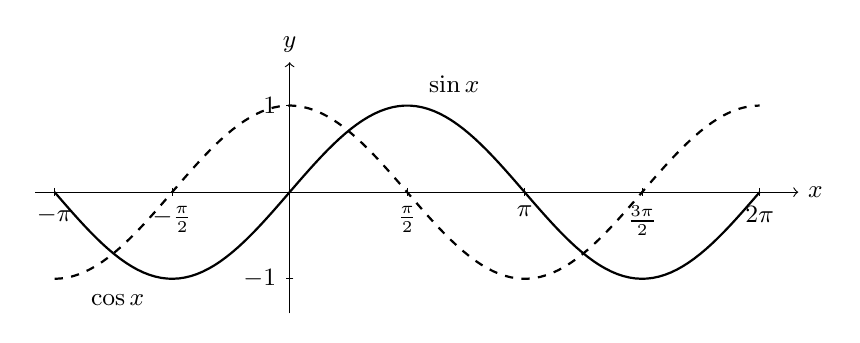
\begin{tikzpicture}[xscale=0.95,yscale=1.1,font=\small]
  \draw[->] (-3.4,0) -- (6.8,0) node[right] {$x$};
  \draw[->] (0,-1.4) -- (0,1.5) node[above] {$y$};
  \foreach \x/\l in {-3.1416/{-\pi},-1.5708/{-\frac{\pi}{2}},1.5708/{\frac{\pi}{2}},3.1416/{\pi},4.7124/{\frac{3\pi}{2}},6.2832/{2\pi}}
    \draw (\x,0.05) -- (\x,-0.05) node[below] {$\l$};
  \draw (0.05,1) -- (-0.05,1) node[left] {$1$};
  \draw (0.05,-1) -- (-0.05,-1) node[left] {$-1$};
  \draw[thick,domain=-3.1416:6.2832,samples=120] plot (\x,{sin(\x r)});
  \draw[thick,dashed,domain=-3.1416:6.2832,samples=120] plot (\x,{cos(\x r)});
  \node at (2.2,1.25) {$\sin x$};
  \node at (-2.3,-1.25) {$\cos x$};
\end{tikzpicture}
\caption{Gráficas de $\sin x$ (trazo continuo) y $\cos x$ (discontinuo) en $[-\pi,2\pi]$.}
\label{fig:graficas}
\end{figure}

\begin{definicion}[Sinusoide]
Una \emph{sinusoide} es una función $y=A\sin\bigl(\omega(x-x_0)\bigr)+D$ con $A\ne0$ y $\omega>0$. Se llaman \emph{amplitud} a $\abs{A}$, \emph{periodo} a $2\pi/\omega$, \emph{frecuencia angular} a $\omega$, \emph{desfase} (desplazamiento horizontal) a $x_0$ y \emph{desplazamiento vertical} a $D$.
\end{definicion}

Por la \cref{prop:periodos}(ii), el periodo de la sinusoide es efectivamente $2\pi/\omega$. Al escribir $y=A\sin(\omega x-c)+D$, el desfase es $x_0=c/\omega$, no $c$.

\begin{proposicion}[Suma de un seno y un coseno]\label{prop:armonico}
Sean $a,b\in\R$ no ambos nulos y $R=\sqrt{a^{2}+b^{2}}$. Existe $\varphi\in(-\pi,\pi]$ con $\cos\varphi=a/R$ y $\sin\varphi=b/R$, y para todo $x$
\[
a\sin x+b\cos x=R\sin(x+\varphi).
\]
En particular, el máximo de $a\sin x+b\cos x$ es $R$ y el mínimo, $-R$.
\end{proposicion}

\begin{proof}
El punto $(a/R,b/R)$ está en la circunferencia unidad, porque $(a^{2}+b^{2})/R^{2}=1$, luego es $P(\varphi)$ para algún $\varphi$, que puede tomarse en $(-\pi,\pi]$. Por el \cref{cor:suma}, $R\sin(x+\varphi)=R\sin x\cos\varphi+R\cos x\sin\varphi=a\sin x+b\cos x$. El valor extremo se sigue de que $\sin(x+\varphi)$ recorre $[-1,1]$.
\end{proof}

\section{Funciones trigonométricas inversas}

Una función periódica no es inyectiva, luego no tiene inversa. Se restringe a un intervalo donde sea biyectiva sobre su imagen~\cite[§8.3]{osat}.

\begin{definicion}[Inversas principales]\label{def:inversas}
\begin{enumerate}
  \item $\sin\colon[-\frac{\pi}{2},\frac{\pi}{2}]\to[-1,1]$ es biyectiva; su inversa es $\arcsin\colon[-1,1]\to[-\frac{\pi}{2},\frac{\pi}{2}]$.
  \item $\cos\colon[0,\pi]\to[-1,1]$ es biyectiva; su inversa es $\arccos\colon[-1,1]\to[0,\pi]$.
  \item $\tan\colon(-\frac{\pi}{2},\frac{\pi}{2})\to\R$ es biyectiva; su inversa es $\arctan\colon\R\to(-\frac{\pi}{2},\frac{\pi}{2})$.
\end{enumerate}
\end{definicion}

La inyectividad de estas restricciones se demuestra en el \cref{eje:4-creciente} (el seno es estrictamente creciente en $[-\frac{\pi}{2},\frac{\pi}{2}]$) y de forma análoga para las otras dos. La sobreyectividad es geométrica: cada recta horizontal $y=t$ con $\abs{t}\le1$ corta la semicircunferencia derecha en un punto, y cada recta vertical $x=t$ corta la superior en un punto; para la tangente, cada recta por el origen no vertical corta la semicircunferencia derecha abierta.

\begin{proposicion}[Propiedades de las inversas]\label{prop:inversas}
\begin{enumerate}
  \item $\sin(\arcsin x)=x$ para $x\in[-1,1]$, y $\arcsin(\sin\theta)=\theta$ si y solo si $\theta\in[-\frac{\pi}{2},\frac{\pi}{2}]$.
  \item $\cos(\arcsin x)=\sqrt{1-x^{2}}$ y $\sin(\arccos x)=\sqrt{1-x^{2}}$ para $x\in[-1,1]$.
  \item $\arcsin x+\arccos x=\frac{\pi}{2}$ para $x\in[-1,1]$.
  \item $\arcsin$ y $\arctan$ son impares, y $\arccos(-x)=\pi-\arccos x$.
\end{enumerate}
\end{proposicion}

\begin{proof}
(i) Es la definición de función inversa; si $\theta\notin[-\frac{\pi}{2},\frac{\pi}{2}]$, $\arcsin(\sin\theta)$ está en ese intervalo y no puede ser $\theta$. (ii) Sea $\theta=\arcsin x\in[-\frac{\pi}{2},\frac{\pi}{2}]$; ahí $\cos\theta\ge0$, luego $\cos\theta=+\sqrt{1-\sin^{2}\theta}=\sqrt{1-x^{2}}$. La segunda es análoga, con $\sin\ge0$ en $[0,\pi]$. (iii) Sea $\theta=\arcsin x$. Entonces $\frac{\pi}{2}-\theta\in[0,\pi]$ y $\cos(\frac{\pi}{2}-\theta)=\sin\theta=x$, luego $\arccos x=\frac{\pi}{2}-\theta$. (iv) Si $\theta=\arcsin x$, entonces $-\theta\in[-\frac{\pi}{2},\frac{\pi}{2}]$ y $\sin(-\theta)=-x$, luego $\arcsin(-x)=-\theta$; igual para $\arctan$. Si $\theta=\arccos x$, entonces $\pi-\theta\in[0,\pi]$ y $\cos(\pi-\theta)=-x$.
\end{proof}

\begin{ejemplo}\label{ej:inversas}
$\arcsin(\sin\frac{5\pi}{6})=\arcsin\frac12=\frac{\pi}{6}\ne\frac{5\pi}{6}$. Por la \cref{prop:inversas}(ii), $\cos(\arcsin\frac35)=\sqrt{1-\frac{9}{25}}=\frac45$.
\end{ejemplo}

\section{Ecuaciones trigonométricas}

\begin{teorema}[Soluciones generales]\label{teo:ecuaciones}
Sea $a\in\R$.
\begin{enumerate}
  \item Si $\abs{a}\le1$ y $\alpha=\arcsin a$, entonces $\sin x=a$ si y solo si $x=\alpha+2k\pi$ o $x=\pi-\alpha+2k\pi$ con $k\in\Z$.
  \item Si $\abs{a}\le1$ y $\beta=\arccos a$, entonces $\cos x=a$ si y solo si $x=\pm\beta+2k\pi$ con $k\in\Z$.
  \item Para todo $a$, $\tan x=a$ si y solo si $x=\arctan a+k\pi$ con $k\in\Z$.
\end{enumerate}
Si $\abs{a}>1$, las ecuaciones $\sin x=a$ y $\cos x=a$ no tienen solución.
\end{teorema}

\begin{proof}
(i) La recta $y=a$ corta la circunferencia unidad en los puntos $P(\alpha)$ y $P(\pi-\alpha)$, que tienen ordenada $a$ por el \cref{teo:simetrias}(iv), y en ningún otro (de $x^{2}=1-a^{2}$ salen a lo sumo dos abscisas, opuestas entre sí, y $P(\alpha)$, $P(\pi-\alpha)$ tienen abscisas $\cos\alpha$ y $-\cos\alpha$). Por tanto $\sin x=a$ si y solo si $P(x)\in\{P(\alpha),P(\pi-\alpha)\}$, y el \cref{teo:simetrias}(ii) traduce esta condición en la del enunciado. (ii) Igual, con la recta vertical $x=a$, que corta en $P(\beta)$ y $P(-\beta)$. (iii) La tangente tiene periodo $\pi$ y es inyectiva en $(-\frac{\pi}{2},\frac{\pi}{2})$; todo $x$ del dominio se escribe de forma única como $x=x_0+k\pi$ con $x_0$ en ese intervalo, y $\tan x=\tan x_0=a$ equivale a $x_0=\arctan a$. La última afirmación se debe a que $\abs{\sin x}\le1$ y $\abs{\cos x}\le1$.
\end{proof}

\begin{ejemplo}[Ecuación de segundo grado en el seno]\label{ej:cuadratica}
Para resolver $2\sin^{2}x+3\sin x+1=0$ en $[0,2\pi)$ se pone $s=\sin x$: $2s^{2}+3s+1=(2s+1)(s+1)=0$, de modo que $s=-\frac12$ o $s=-1$. Con el \cref{teo:ecuaciones}, $\sin x=-\frac12$ da $x=\frac{7\pi}{6}$ y $x=\frac{11\pi}{6}$, y $\sin x=-1$ da $x=\frac{3\pi}{2}$.
\end{ejemplo}

\begin{observacion}[Errores frecuentes]
(a) Dar solo $\arcsin a$ como solución de $\sin x=a$ y perder la familia $\pi-\arcsin a+2k\pi$. (b) Dividir ambos miembros por $\cos x$ o $\sin x$ sin estudiar aparte el caso en que se anulan: en $\sin2x=\cos x$ se pierden las soluciones con $\cos x=0$ (\cref{eje:4-doble}). (c) Elevar al cuadrado introduce soluciones falsas que deben descartarse sustituyendo (\cref{eje:4-cuadrado}). (d) Confundir el desfase $c$ de $\sin(\omega x-c)$ con el desplazamiento horizontal $c/\omega$.
\end{observacion}

\begin{observacion}[Conexión con el curso]
La codificación sinusoidal del Transformer~\cite[§3.5]{vaswani} asigna a la posición $p$ el vector con componentes $\PE(p)_{2i}=\sin(p\,\omega_i)$ y $\PE(p)_{2i+1}=\cos(p\,\omega_i)$, con frecuencias $\omega_i=10000^{-2i/d}$ (módulo~14, tema~4). Cada par de componentes es una sinusoide de la posición con periodo $2\pi/\omega_i$, y los periodos forman una progresión geométrica desde $2\pi$ hasta casi $2\pi\cdot10^{4}$. Las mismas frecuencias, con el nombre de longitudes de onda $\lambda_i=2\pi/\theta_i$, gobiernan la extensión del contexto de RoPE en el módulo~18 (tema~3).
\end{observacion}

\begin{lecturas}
\item OpenStax, \emph{Algebra and Trigonometry}~\cite{osat}, §8.1 «Graphs of the Sine and Cosine Functions», §8.2 «Graphs of the Other Trigonometric Functions», §8.3 «Inverse Trigonometric Functions» y §9.5 «Solving Trigonometric Equations».
\item Vaswani \emph{et al.}~\cite{vaswani}, §3.5 «Positional Encoding».
\end{lecturas}

\section*{Ejercicios del tema 4}
\addcontentsline{toc}{section}{Ejercicios del tema 4}

\begin{ejercicio}{1}{eje:4-parametros}
Para $y=3\sin(2x-\frac{\pi}{3})+1$, determine la amplitud, el periodo, el desplazamiento horizontal, el desplazamiento vertical y los valores máximo y mínimo.
\fuente{adaptado de OpenStax, \emph{Algebra and Trigonometry}~\cite{osat}, §8.1, ejercicios de la sección sobre amplitud, periodo y desfase.}
\end{ejercicio}

\begin{ejercicio}{1}{eje:4-dominios}
(a) Escriba el dominio y la imagen de $\arcsin$, $\arccos$ y $\arctan$, y explique por qué hay que restringir el dominio del seno antes de invertirlo. (b) Calcule $\arcsin(\sin\frac{3\pi}{4})$, $\arccos(\cos(-\frac{\pi}{3}))$ y $\tan(\arctan5)$.
\end{ejercicio}

\begin{ejercicio}{2}{eje:4-exactos}
Calcule el valor exacto de: (a)~$\arcsin(-\frac12)$; (b)~$\arccos(-\frac{\sqrt2}{2})$; (c)~$\arctan\sqrt3$; (d)~$\arccos(\cos\frac{5\pi}{3})$; (e)~$\sin(\arccos\frac35)$; (f)~$\tan(\arcsin\frac13)$.
\fuente{adaptado de OpenStax, \emph{Algebra and Trigonometry}~\cite{osat}, §8.3, ejercicios de la sección sobre evaluación y composición de inversas.}
\end{ejercicio}

\begin{ejercicio}{2}{eje:4-basicas}
Resuelva: (a) $2\sin x-1=0$, en $[0,2\pi)$ y en general; (b) $\tan x=-\sqrt3$, en general; (c) $\cos2x=\frac12$, en $[0,2\pi)$.
\fuente{adaptado de OpenStax, \emph{Algebra and Trigonometry}~\cite{osat}, §9.5, ejercicios de la sección sobre ecuaciones lineales en una función trigonométrica.}
\end{ejercicio}

\begin{ejercicio}{2}{eje:4-cuadratica}
Resuelva $2\cos^{2}x-\cos x-1=0$ en $\R$.
\fuente{adaptado de OpenStax, \emph{Algebra and Trigonometry}~\cite{osat}, §9.5, ejercicios de la sección sobre ecuaciones de tipo cuadrático.}
\end{ejercicio}

\begin{ejercicio}{2}{eje:4-doble}
Resuelva $\sin2x=\cos x$ en $[0,2\pi)$. Explique qué soluciones se perderían al dividir por $\cos x$.
\end{ejercicio}

\begin{ejercicio}{2}{eje:4-armonico}
Escriba $\sqrt3\sin x+\cos x$ en la forma $R\sin(x+\varphi)$, determine su máximo y dónde se alcanza en $[0,2\pi)$, y resuelva $\sqrt3\sin x+\cos x=1$ en $[0,2\pi)$.
\end{ejercicio}

\begin{ejercicio}{2}{eje:4-cuadrado}
Resuelva $\sin x+\cos x=1$ en $[0,2\pi)$ de dos maneras: (a) elevando al cuadrado y comprobando las soluciones obtenidas; (b) con la \cref{prop:armonico}. Explique por qué el método (a) produce soluciones falsas.
\end{ejercicio}

\begin{ejercicio}{2}{eje:4-periodo-suma}
Determine el periodo fundamental de $f(x)=\sin3x+\cos2x$ y de $g(x)=\sin^{2}x$. Para $f$, basta probar que $2\pi$ es periodo y que ningún $0<T<2\pi$ lo es; para esto último, estudie $f(T)$ y $f(-T)$ frente a $f(0)$.
\end{ejercicio}

\begin{ejercicio}{2}{eje:4-pe}
Sea $d=8$ y $\omega_i=10000^{-2i/d}$ para $i=0,1,2,3$. Calcule las cuatro frecuencias, los periodos $2\pi/\omega_i$ y el vector $\PE(1)\in\R^{8}$ con cuatro decimales. ¿Qué componentes distinguen bien las posiciones $1$ y $2$, y cuáles apenas cambian?
\fuente{definición de Vaswani \emph{et al.}~\cite[§3.5]{vaswani}; datos elegidos para el cálculo a mano.}
\end{ejercicio}

\begin{ejercicio}{3}{eje:4-creciente}
Demuestre que el seno es estrictamente creciente en $[-\frac{\pi}{2},\frac{\pi}{2}]$, y por tanto inyectivo en ese intervalo. Indicación: para $a>b$ en el intervalo, escriba $\sin a-\sin b$ como producto (\cref{cor:suma-producto}) y estudie el signo de cada factor.
\end{ejercicio}

\begin{ejercicio}{3}{eje:4-cos-iguales}
Demuestre que $\cos x=\cos y$ si y solo si $x=y+2k\pi$ o $x=-y+2k\pi$ para algún $k\in\Z$, usando la fórmula de $\cos x-\cos y$ como producto y el \cref{eje:1-periodo-tan}(a).
\end{ejercicio}

\begin{ejercicio}{3}{eje:4-arctan-inverso}
Demuestre que $\arctan x+\arctan\frac1x=\frac{\pi}{2}$ si $x>0$ y $-\frac{\pi}{2}$ si $x<0$.
\end{ejercicio}

\begin{ejercicio}{3}{eje:4-machin}
Demuestre que $\arctan\frac12+\arctan\frac13=\frac{\pi}{4}$. Justifique con cuidado por qué basta comprobar que la tangente de ambos miembros coincide.
\end{ejercicio}

\begin{ejercicio}{3}{eje:4-pe-lineal}
Sea $\omega>0$ y $v(p)=(\sin\omega p,\ \cos\omega p)\T$. Demuestre que para cada $k\in\R$ existe una matriz $M_k\in\R^{2\times2}$, que depende de $k$ y $\omega$ pero no de $p$, tal que $v(p+k)=M_kv(p)$ para todo $p$. Demuestre que $M_k$ es ortogonal ($M_k\T M_k=I$) y que $M_kM_l=M_{k+l}$.
\fuente{adaptado de la propiedad enunciada sin demostración por Vaswani \emph{et al.}~\cite[§3.5]{vaswani}.}
\end{ejercicio}

% =====================================================================
\chapter{Números complejos en forma binómica}
\label{tema:5}
% =====================================================================

Los números complejos amplían los reales con una raíz cuadrada de $-1$. Con ellos toda ecuación polinómica tiene solución, y las operaciones de giro y homotecia del plano se escriben como productos. Este tema construye $\C$, demuestra las propiedades del conjugado y del módulo y resuelve ecuaciones de segundo grado con coeficientes complejos. Se sigue la §2.4 de~\cite{osat}, la sección~5 de las notas de 18.03 del MIT~\cite{mit1803} y la §1.1 de las notas de «Vectors and Matrices» de Cambridge~\cite{cambvm}.

\section{El cuerpo de los números complejos}

\begin{definicion}[Números complejos]\label{def:complejos}
Un \emph{número complejo} es una expresión $z=a+bi$ con $a,b\in\R$; se llaman \emph{parte real} $\Real z=a$ y \emph{parte imaginaria} $\Imag z=b$. Dos complejos son iguales si tienen iguales las partes reales y las imaginarias. Con $z=a+bi$ y $w=c+di$ se definen
\[
z+w=(a+c)+(b+d)i,\qquad zw=(ac-bd)+(ad+bc)i .
\]
El conjunto de los números complejos se denota $\C$. Se identifica el real $a$ con $a+0i$, y se escribe $i=0+1i$.
\end{definicion}

La regla del producto es la que resulta de operar como con polinomios en $i$ y sustituir $i^{2}=-1$: en efecto, con la definición, $i\cdot i=(0\cdot0-1\cdot1)+(0\cdot1+1\cdot0)i=-1$. Geométricamente, $a+bi$ se representa como el punto $(a,b)$ del \emph{plano complejo}, con el eje real horizontal y el imaginario vertical (\cref{fig:argand}).

\begin{teorema}\label{teo:cuerpo}
Con estas operaciones, $\C$ es un cuerpo: la suma y el producto son asociativos y conmutativos, el producto es distributivo respecto de la suma, $0$ y $1$ son los elementos neutros, y todo $z=a+bi\ne0$ tiene inverso
\[
z^{-1}=\frac{a}{a^{2}+b^{2}}-\frac{b}{a^{2}+b^{2}}\,i .
\]
\end{teorema}

\begin{proof}
Las propiedades de la suma son las de $\R^{2}$ componente a componente. La conmutatividad del producto se ve en la fórmula, simétrica en $(a,b)$ y $(c,d)$; la asociatividad y la distributividad se comprueban desarrollando ambos miembros (el cálculo, rutinario, se propone en~\cite[§5.1]{mit1803}). Para el inverso, si $z\ne0$ entonces $a^{2}+b^{2}>0$ y
\[
(a+bi)\Bigl(\frac{a}{a^{2}+b^{2}}-\frac{b}{a^{2}+b^{2}}i\Bigr)=\frac{a^{2}+b^{2}}{a^{2}+b^{2}}+\frac{-ab+ab}{a^{2}+b^{2}}\,i=1.\qedhere
\]
\end{proof}

\begin{ejemplo}[Potencias de $i$]\label{ej:potencias-i}
$i^{1}=i$, $i^{2}=-1$, $i^{3}=-i$, $i^{4}=1$, y a partir de ahí se repiten: $i^{n}$ solo depende del resto de dividir $n$ entre~4. Por ejemplo, $i^{103}=i^{4\cdot25+3}=i^{3}=-i$.
\end{ejemplo}

\section{El conjugado}

\begin{definicion}[Conjugado]
El \emph{conjugado} de $z=a+bi$ es $\bar z=a-bi$. Geométricamente, es la reflexión de $z$ en el eje real.
\end{definicion}

\begin{proposicion}[Propiedades del conjugado]\label{prop:conjugado}
Para todos $z,w\in\C$:
\begin{enumerate}
  \item $\overline{z+w}=\bar z+\bar w$, \quad $\overline{zw}=\bar z\,\bar w$, \quad $\overline{z/w}=\bar z/\bar w$ si $w\ne0$, \quad $\bar{\bar z}=z$;
  \item $z+\bar z=2\Real z$ y $z-\bar z=2i\Imag z$;
  \item $z$ es real si y solo si $z=\bar z$;
  \item $z\bar z=(\Real z)^{2}+(\Imag z)^{2}$, que es un número real mayor o igual que~0.
\end{enumerate}
\end{proposicion}

\begin{proof}
Sean $z=a+bi$ y $w=c+di$. (i) $\overline{z+w}=(a+c)-(b+d)i=\bar z+\bar w$. Para el producto, $\overline{zw}=(ac-bd)-(ad+bc)i$, y $\bar z\bar w=(a-bi)(c-di)=(ac-bd)+(-ad-bc)i$, que es lo mismo. Para el cociente, $\bar w\,\overline{(z/w)}=\overline{w\cdot(z/w)}=\bar z$. (ii) y (iii) son inmediatas. (iv) $(a+bi)(a-bi)=a^{2}-(bi)^{2}=a^{2}+b^{2}$.
\end{proof}

La propiedad~(iv) da el método práctico para dividir: se multiplican numerador y denominador por el conjugado del denominador,
\[
\frac{z}{w}=\frac{z\,\bar w}{w\,\bar w}=\frac{z\,\bar w}{c^{2}+d^{2}} .
\]

\begin{ejemplo}\label{ej:division}
$\dfrac{3+i}{1-2i}=\dfrac{(3+i)(1+2i)}{1+4}=\dfrac{3+6i+i+2i^{2}}{5}=\dfrac{1+7i}{5}=\dfrac15+\dfrac75i$.
\end{ejemplo}

\section{El módulo}

\begin{definicion}[Módulo]
El \emph{módulo} de $z=a+bi$ es $\abs{z}=\sqrt{a^{2}+b^{2}}=\sqrt{z\bar z}$, la distancia de $z$ al origen. La distancia entre $z$ y $w$ es $\abs{z-w}$.
\end{definicion}

\begin{proposicion}[Propiedades del módulo]\label{prop:modulo}
Para todos $z,w\in\C$:
\begin{enumerate}
  \item $\abs{z}\ge0$, con igualdad si y solo si $z=0$; \quad $\abs{\bar z}=\abs{z}$;
  \item $\abs{\Real z}\le\abs{z}$ y $\abs{\Imag z}\le\abs{z}$;
  \item $\abs{zw}=\abs{z}\abs{w}$ y, si $w\ne0$, $\abs{z/w}=\abs{z}/\abs{w}$;
  \item (desigualdad triangular) $\abs{z+w}\le\abs{z}+\abs{w}$;
  \item $\bigl|\abs{z}-\abs{w}\bigr|\le\abs{z-w}$.
\end{enumerate}
\end{proposicion}

\begin{proof}
(i) y (ii) se leen en la fórmula: $a^{2}\le a^{2}+b^{2}$. (iii) Por la \cref{prop:conjugado}, $\abs{zw}^{2}=zw\,\overline{zw}=z\bar z\,w\bar w=\abs{z}^{2}\abs{w}^{2}$, y se toman raíces no negativas; el cociente se sigue de aplicar lo anterior a $(z/w)\cdot w=z$. (iv) Por la \cref{prop:conjugado}(ii), $z\bar w+\bar zw=z\bar w+\overline{z\bar w}=2\Real(z\bar w)$, luego
\[
\abs{z+w}^{2}=(z+w)(\bar z+\bar w)=\abs{z}^{2}+\abs{w}^{2}+2\Real(z\bar w)\le\abs{z}^{2}+\abs{w}^{2}+2\abs{z\bar w}=(\abs{z}+\abs{w})^{2},
\]
usando (ii) y (iii). (v) Por (iv), $\abs{z}=\abs{(z-w)+w}\le\abs{z-w}+\abs{w}$, luego $\abs{z}-\abs{w}\le\abs{z-w}$; intercambiando los papeles, $\abs{w}-\abs{z}\le\abs{z-w}$.
\end{proof}

\section{Ecuaciones polinómicas}

\begin{proposicion}[Raíces cuadradas]\label{prop:raiz-cuadrada}
Sea $w=a+bi$ con $b\ne0$. Las soluciones de $z^{2}=w$ son $z=\pm(x+yi)$ con
\[
x=\sqrt{\frac{\abs{w}+a}{2}},\qquad y=\operatorname{signo}(b)\sqrt{\frac{\abs{w}-a}{2}} .
\]
\end{proposicion}

\begin{proof}
Con $z=x+yi$, la ecuación $z^{2}=w$ equivale a $x^{2}-y^{2}=a$ y $2xy=b$. Tomando módulos, $\abs{z}^{2}=\abs{w}$, es decir, $x^{2}+y^{2}=\abs{w}$. Sumando y restando con la primera ecuación, $x^{2}=\frac{\abs{w}+a}{2}$ e $y^{2}=\frac{\abs{w}-a}{2}$, ambos positivos porque $\abs{w}>\abs{a}$ cuando $b\ne0$. La condición $2xy=b$ fija que $x$ e $y$ tengan el producto del signo de $b$, lo que deja exactamente los dos pares del enunciado; y estos pares la cumplen, porque $(2xy)^{2}=4\cdot\frac{\abs{w}^{2}-a^{2}}{4}=b^{2}$.
\end{proof}

\begin{ejemplo}\label{ej:raiz}
Para $w=3+4i$, $\abs{w}=5$, $x=\sqrt{4}=2$, $y=\sqrt1=1$: las raíces son $\pm(2+i)$. Comprobación: $(2+i)^{2}=4+4i+i^{2}=3+4i$.
\end{ejemplo}

\begin{proposicion}[Fórmula cuadrática en $\C$]\label{prop:cuadratica}
Sean $a,b,c\in\C$ con $a\ne0$, y sea $\delta\in\C$ con $\delta^{2}=b^{2}-4ac$. Las soluciones de $az^{2}+bz+c=0$ son $z=\dfrac{-b\pm\delta}{2a}$.
\end{proposicion}

\begin{proof}
Multiplicando por $4a\ne0$ y completando el cuadrado, la ecuación equivale a $(2az+b)^{2}=b^{2}-4ac=\delta^{2}$, es decir, $(2az+b-\delta)(2az+b+\delta)=0$. Como $\C$ es un cuerpo, un producto es nulo si y solo si lo es algún factor, de donde $2az+b=\pm\delta$.
\end{proof}

\begin{proposicion}[Raíces conjugadas]\label{prop:conjugadas}
Si $p(z)=\sum_{k=0}^{n}c_kz^{k}$ tiene coeficientes reales, entonces $p(\bar z)=\overline{p(z)}$ para todo $z$. En particular, si $z$ es raíz de $p$, también lo es $\bar z$.
\end{proposicion}

\begin{proof}
Por la \cref{prop:conjugado}(i), aplicada repetidamente, $\overline{z^{k}}=\bar z^{k}$ y $\overline{\sum c_kz^{k}}=\sum\bar c_k\bar z^{k}=\sum c_k\bar z^{k}$, porque $\bar c_k=c_k$. Si $p(z)=0$, entonces $p(\bar z)=\bar0=0$.
\end{proof}

\begin{teorema}[Teorema fundamental del álgebra]\label{teo:fundamental}
Todo polinomio de grado $n\ge1$ con coeficientes complejos tiene al menos una raíz en $\C$. En consecuencia, se factoriza como $c\prod_{k=1}^{n}(z-z_k)$ y tiene exactamente $n$ raíces contadas con multiplicidad.
\end{teorema}

La demostración requiere herramientas de análisis y se omite; véanse~\cite[§5.3]{mit1803} y~\cite{needham}. La consecuencia se obtiene por inducción sobre $n$, dividiendo por $z-z_1$ cada vez que se encuentra una raíz.

\section{El plano complejo y el producto escalar}

\begin{figure}[ht]
\centering
\begin{tikzpicture}[scale=1.1,font=\small,>={Stealth[length=2mm]}]
  \draw[->] (-1.2,0) -- (4.2,0) node[right] {$\Real$};
  \draw[->] (0,-2.4) -- (0,2.8) node[above] {$\Imag$};
  \coordinate (z) at (3,2);
  \coordinate (zb) at (3,-2);
  \draw[thick,->] (0,0) -- (z);
  \draw[thick,->,dashed] (0,0) -- (zb);
  \draw[dotted] (z) -- (3,0) node[below right] {$a$};
  \draw[dotted] (z) -- (0,2) node[left] {$b$};
  \fill (z) circle (0.05) node[above right] {$z=a+bi$};
  \fill (zb) circle (0.05) node[below right] {$\bar z=a-bi$};
  \node at (1.25,1.25) [rotate=33.7] {$\abs{z}$};
\end{tikzpicture}
\caption{El plano complejo. El número $z=a+bi$ es el punto $(a,b)$; su módulo es la distancia al origen y su conjugado, la reflexión en el eje real.}
\label{fig:argand}
\end{figure}

Al identificar $\C$ con $\R^{2}$, la suma de complejos es la suma de vectores, y el producto por un real $\lambda$ es el producto de un vector por un escalar. El producto de dos complejos no tiene análogo en $\R^{2}$ y es el objeto del \cref{tema:6}. El conjugado permite recuperar el producto escalar y el área orientada:

\begin{proposicion}\label{prop:escalar-complejo}
Sean $z=a+bi$ y $w=c+di$, identificados con $u=(a,b)$ y $v=(c,d)$. Entonces
\[
\Real(z\bar w)=ac+bd=u\cdot v,\qquad \Imag(\bar z w)=ad-bc=\det\begin{pmatrix}a&c\\ b&d\end{pmatrix}.
\]
\end{proposicion}

\begin{proof}
$z\bar w=(a+bi)(c-di)=(ac+bd)+(bc-ad)i$ y $\bar zw=(a-bi)(c+di)=(ac+bd)+(ad-bc)i$.
\end{proof}

\begin{observacion}[Errores frecuentes]
(a) La parte imaginaria de $a+bi$ es el número real $b$, no $bi$. (b) $\abs{z}^{2}=z\bar z$, pero en general $\abs{z}^{2}\ne z^{2}$: para $z=i$, $\abs{z}^{2}=1$ y $z^{2}=-1$. (c) La regla $\sqrt{zw}=\sqrt z\sqrt w$ falla en $\C$: con $z=w=-1$ daría $1=\sqrt1=\sqrt{-1}\sqrt{-1}=i^{2}=-1$. Todo número complejo no nulo tiene dos raíces cuadradas y no hay una elección de signo compatible con el producto. (d) En $\C$ no hay un orden compatible con las operaciones (\cref{eje:5-orden}): no tiene sentido escribir $z<w$ entre complejos no reales.
\end{observacion}

\begin{observacion}[Conexión con el curso]
Una matriz real puede tener autovalores complejos, y por la \cref{prop:conjugadas} aparecen en pares conjugados, porque el polinomio característico tiene coeficientes reales (módulo~3, tema~3). La \cref{prop:escalar-complejo} es la identidad que usa la forma compleja de RoPE (módulo~14, tema~4): cada par de coordenadas $(q_{2j},q_{2j+1})$ de una consulta se trata como un número complejo, y el producto escalar de dos pares es $\Real(z\bar w)$.
\end{observacion}

\begin{lecturas}
\item OpenStax, \emph{Algebra and Trigonometry}~\cite{osat}, §2.4 «Complex Numbers».
\item MIT 18.03, \emph{Supplementary Notes}~\cite{mit1803}, §5 «The algebra of complex numbers» (5.1 a 5.3).
\item Cambridge, \emph{Vectors and Matrices}~\cite{cambvm}, §1.1 «Basic properties».
\end{lecturas}

\section*{Ejercicios del tema 5}
\addcontentsline{toc}{section}{Ejercicios del tema 5}

\begin{ejercicio}{1}{eje:5-partes}
Para $z_1=3-4i$, $z_2=-2i$, $z_3=5$ y $z_4=-1+i$, indique la parte real, la parte imaginaria, el conjugado y el módulo, y sitúe cada número en el plano complejo.
\end{ejercicio}

\begin{ejercicio}{1}{eje:5-vf}
Justifique si son verdaderas o falsas para todos $z,w\in\C$: (a) $\abs{z+w}=\abs{z}+\abs{w}$; (b) $z\bar z$ es real y no negativo; (c) $\overline{z^{2}}=\bar z^{\,2}$; (d) $\Imag(3+2i)=2i$.
\end{ejercicio}

\begin{ejercicio}{1}{eje:5-potencias-i}
Calcule $i^{7}$, $i^{100}$, $i^{-1}$ e $i^{2026}$, y la suma $1+i+i^{2}+\dots+i^{10}$.
\end{ejercicio}

\begin{ejercicio}{2}{eje:5-operaciones}
Escriba en forma binómica $(3+2i)(1-4i)$, $(2-i)^{2}$, $\dfrac{2-i}{1+3i}$ y $(1+i)^{4}$.
\fuente{adaptado de OpenStax, \emph{Algebra and Trigonometry}~\cite{osat}, §2.4, ejercicios de la sección sobre operaciones con complejos.}
\end{ejercicio}

\begin{ejercicio}{2}{eje:5-inversos}
Calcule $i^{-1}$, $(1+i)^{-1}$ y $\dfrac{1+i}{2-i}$, y exprese $\abs{z^{-1}}$ en función de $\abs{z}$.
\fuente{adaptado de MIT 18.03, \emph{Supplementary Notes}~\cite{mit1803}, ejercicio~5.2.3.}
\end{ejercicio}

\begin{ejercicio}{2}{eje:5-cuadraticas}
Encuentre las raíces de $x^{2}+x+1$ y de $x^{2}+x+2$, y resuelva $x^{2}+ix+1=0$.
\fuente{adaptado de MIT 18.03, \emph{Supplementary Notes}~\cite{mit1803}, ejercicio~5.2.4.}
\end{ejercicio}

\begin{ejercicio}{2}{eje:5-suma-tripos}
Sean $x,y\in\R$ tales que $x+iy=\sum_{a=0}^{200}i^{a}+\sum_{b=1}^{50}i^{b}$. Calcule $xy$.
\fuente{adaptado de Cambridge, \emph{Mathematical Tripos} Part IA, Paper~1, 2019~\cite{tripos2019}, pregunta~1C(a).}
\end{ejercicio}

\begin{ejercicio}{2}{eje:5-raices-cuadradas}
Calcule las raíces cuadradas de $-5+12i$ y de $-2i$ con la \cref{prop:raiz-cuadrada}, y compruébelas elevando al cuadrado.
\end{ejercicio}

\begin{ejercicio}{2}{eje:5-cuadratica-compleja}
Resuelva $z^{2}-(3+i)z+(2+2i)=0$ y compruebe que la suma y el producto de las raíces son los esperados.
\end{ejercicio}

\begin{ejercicio}{2}{eje:5-lugares}
Describa geométricamente y dibuje los conjuntos (a) $\{z:\abs{z-1}=\abs{z+i}\}$ y (b) $\{z:\abs{z+3i}=3\abs{z}\}$.
\fuente{el apartado (b) está adaptado de Cambridge, \emph{Mathematical Tripos} Part IA, Paper~1, 2013~\cite{tripos2013}, pregunta~1C(b).}
\end{ejercicio}

\begin{ejercicio}{2}{eje:5-escalar}
Sean $z=1+2i$ y $w=3+i$. Calcule $z\bar w$ y compruebe la \cref{prop:escalar-complejo}: $\Real(z\bar w)$ es el producto escalar de $(1,2)$ y $(3,1)$. Calcule también el ángulo entre ambos vectores.
\end{ejercicio}

\begin{ejercicio}{3}{eje:5-modulo-producto}
Demuestre directamente, sin usar el conjugado, que si $z=a+bi$ entonces $z\bar z=a^{2}+b^{2}$ y que $\abs{wz}=\abs{w}\abs{z}$ desarrollando ambos miembros en coordenadas. ¿Qué identidad entre números reales se obtiene?
\fuente{adaptado de MIT 18.03, \emph{Supplementary Notes}~\cite{mit1803}, ejercicios~5.2.1 y~5.2.2.}
\end{ejercicio}

\begin{ejercicio}{3}{eje:5-igualdad-triangular}
Demuestre que, para $z,w\ne0$, se cumple $\abs{z+w}=\abs{z}+\abs{w}$ si y solo si $w=\lambda z$ para algún real $\lambda>0$.
\end{ejercicio}

\begin{ejercicio}{3}{eje:5-orden}
Demuestre que no existe en $\C$ un orden total $<$ compatible con las operaciones, es decir, que cumpla: si $z<w$ entonces $z+u<w+u$ para todo $u$, y si $0<z$ y $0<w$ entonces $0<zw$. Indicación: en un orden así, todo cuadrado no nulo es positivo.
\end{ejercicio}

\begin{ejercicio}{3}{eje:5-blaschke}
Sean $z,w\in\C$ con $\abs{z}=1$ y $\bar wz\ne1$. Demuestre que $\left|\dfrac{z-w}{1-\bar wz}\right|=1$.
\end{ejercicio}

% =====================================================================
\chapter{Forma polar, fórmula de Euler, De Moivre y rotaciones}
\label{tema:6}
% =====================================================================

La forma binómica es cómoda para sumar; la forma polar, para multiplicar. Este tema demuestra que al multiplicar dos complejos se multiplican los módulos y se suman los argumentos, introduce la exponencial imaginaria $e^{i\theta}$ y la fórmula de Euler, deduce el teorema de De Moivre y la fórmula de las raíces $n$-ésimas, y termina interpretando la multiplicación por $e^{i\alpha}$ como el giro de ángulo $\alpha$ del plano, que es la idea sobre la que se construye RoPE. Se siguen la sección~6 de las notas de 18.03 del MIT~\cite{mit1803}, las §1.2 a §1.5 de las notas de Cambridge~\cite{cambvm}, la §10.5 de~\cite{osat} y la lectura geométrica del capítulo~1 de Needham~\cite{needham}.

\section{Argumento y forma polar}

\begin{definicion}[Argumento y forma polar]\label{def:polar}
Sea $z\ne0$ y $r=\abs{z}$. Un \emph{argumento} de $z$ es cualquier $\theta\in\R$ tal que
\[
z=r(\cos\theta+i\sin\theta).
\]
Esta expresión es la \emph{forma polar} de $z$. El \emph{argumento principal} $\Arg z$ es el único argumento en $(-\pi,\pi]$. El número $0$ no tiene argumento.
\end{definicion}

Todo $z\ne0$ tiene argumento: $z/r$ tiene módulo~1, luego es un punto $P(\theta)$ de la circunferencia unidad. Por el \cref{teo:simetrias}(ii), dos argumentos de $z$ difieren en un múltiplo entero de $2\pi$, y exactamente uno está en $(-\pi,\pi]$.

\begin{proposicion}[Cálculo del argumento principal]\label{prop:arg}
Sea $z=a+bi\ne0$. Si $a>0$, $\Arg z=\arctan(b/a)$. Si $a<0$, $\Arg z=\arctan(b/a)+\pi$ cuando $b\ge0$ y $\arctan(b/a)-\pi$ cuando $b<0$. Si $a=0$, $\Arg z=\pi/2$ cuando $b>0$ y $-\pi/2$ cuando $b<0$.
\end{proposicion}

\begin{proof}
Si $\theta$ es un argumento, $\cos\theta=a/r$ y $\sin\theta=b/r$, luego $\tan\theta=b/a$ cuando $a\ne0$. Si $a>0$, $\theta$ está en el cuadrante I o IV y $\arctan(b/a)\in(-\frac{\pi}{2},\frac{\pi}{2})$ es el argumento correcto. Si $a<0$, $\arctan(b/a)$ apunta al cuadrante opuesto y hay que sumar o restar $\pi$ (\cref{teo:simetrias}(v)), eligiendo el signo que deja el resultado en $(-\pi,\pi]$. El caso $a=0$ es directo.
\end{proof}

\begin{ejemplo}\label{ej:polar}
Para $z=-1+\sqrt3\,i$: $r=\sqrt{1+3}=2$ y, como $a<0\le b$, $\Arg z=\arctan(-\sqrt3)+\pi=-\frac{\pi}{3}+\pi=\frac{2\pi}{3}$. Luego $z=2\bigl(\cos\frac{2\pi}{3}+i\sin\frac{2\pi}{3}\bigr)$.
\end{ejemplo}

\section{El producto en forma polar}

\begin{teorema}[Producto y cociente en forma polar]\label{teo:producto-polar}
Sean $z_1=r_1(\cos\theta_1+i\sin\theta_1)$ y $z_2=r_2(\cos\theta_2+i\sin\theta_2)$. Entonces
\[
z_1z_2=r_1r_2\bigl(\cos(\theta_1+\theta_2)+i\sin(\theta_1+\theta_2)\bigr),
\]
y, si $z_2\ne0$, $\dfrac{z_1}{z_2}=\dfrac{r_1}{r_2}\bigl(\cos(\theta_1-\theta_2)+i\sin(\theta_1-\theta_2)\bigr)$.
\end{teorema}

\begin{proof}
Desarrollando el producto y aplicando el \cref{cor:suma},
\[
(\cos\theta_1+i\sin\theta_1)(\cos\theta_2+i\sin\theta_2)=(\cos\theta_1\cos\theta_2-\sin\theta_1\sin\theta_2)+i(\sin\theta_1\cos\theta_2+\cos\theta_1\sin\theta_2),
\]
que es $\cos(\theta_1+\theta_2)+i\sin(\theta_1+\theta_2)$. Para el cociente, el número $w=\frac{r_1}{r_2}(\cos(\theta_1-\theta_2)+i\sin(\theta_1-\theta_2))$ cumple $wz_2=z_1$ por la primera parte, y el cociente es único porque $\C$ es un cuerpo.
\end{proof}

\begin{corolario}\label{cor:arg-producto}
Para $z,w\ne0$: $\abs{zw}=\abs{z}\abs{w}$ y $\arg(zw)=\arg z+\arg w$, en el sentido de que la suma de un argumento de $z$ y uno de $w$ es un argumento de $zw$. Para los argumentos principales, la igualdad solo vale salvo un múltiplo de $2\pi$.
\end{corolario}

\emph{Interpretación geométrica.} Fijado $w=\rho(\cos\alpha+i\sin\alpha)$, la aplicación $z\mapsto wz$ multiplica el módulo de cada punto por $\rho$ y suma $\alpha$ a su argumento: es la composición de un giro de ángulo $\alpha$ alrededor del origen y una homotecia de razón $\rho$. Esta lectura, que Needham sitúa en el centro de su exposición~\cite[cap.~1]{needham}, convierte en evidentes muchas identidades: por ejemplo, multiplicar por $i$ es girar un ángulo recto, y por eso $i^{2}=-1$ (dos giros rectos forman media vuelta).

\section{La exponencial imaginaria y la fórmula de Euler}

\begin{definicion}[Exponencial imaginaria]\label{def:euler}
Para $\theta\in\R$ se define
\[
e^{i\theta}=\cos\theta+i\sin\theta,
\]
y, para $z=x+iy\in\C$, $e^{z}=e^{x}e^{iy}=e^{x}(\cos y+i\sin y)$.
\end{definicion}

La notación no es arbitraria. Si se sustituye formalmente $x=i\theta$ en la serie $e^{x}=\sum_{n\ge0}x^{n}/n!$ y se agrupan los términos pares e impares usando $i^{2}=-1$, se obtienen exactamente las series de $\cos\theta$ y de $i\sin\theta$; las notas de Cambridge toman la serie como definición de $e^{z}$ y deducen la fórmula anterior~\cite[§1.2]{cambvm}. Las notas de 18.03 la justifican de otro modo: $f(\theta)=\cos\theta+i\sin\theta$ es la única función con $f'=if$ y $f(0)=1$, la misma ecuación que caracteriza a $e^{i\theta}$~\cite[§6.2]{mit1803}. Ambos argumentos requieren cálculo; aquí basta la definición y sus propiedades algebraicas.

\begin{proposicion}[Propiedades de $e^{i\theta}$]\label{prop:exp}
Para todos $\alpha,\beta,\theta\in\R$ y $n\in\Z$:
\begin{enumerate}
  \item $e^{i\alpha}e^{i\beta}=e^{i(\alpha+\beta)}$ y, más en general, $e^{z}e^{w}=e^{z+w}$ para $z,w\in\C$;
  \item $\abs{e^{i\theta}}=1$ y $\overline{e^{i\theta}}=e^{-i\theta}=1/e^{i\theta}$;
  \item $e^{i\theta}=1$ si y solo si $\theta\in2\pi\Z$; en particular, $e^{i\pi}=-1$ (identidad de Euler) y $e^{2\pi i}=1$;
  \item $\cos\theta=\dfrac{e^{i\theta}+e^{-i\theta}}{2}$ y $\sin\theta=\dfrac{e^{i\theta}-e^{-i\theta}}{2i}$.
\end{enumerate}
\end{proposicion}

\begin{proof}
(i) La primera igualdad es el \cref{teo:producto-polar} con $r_1=r_2=1$. Para $z=x+iy$ y $w=u+iv$, $e^{z}e^{w}=e^{x}e^{u}e^{iy}e^{iv}=e^{x+u}e^{i(y+v)}=e^{z+w}$, usando la propiedad de la exponencial real. (ii) $\abs{e^{i\theta}}^{2}=\cos^{2}\theta+\sin^{2}\theta=1$; $\overline{e^{i\theta}}=\cos\theta-i\sin\theta=\cos(-\theta)+i\sin(-\theta)=e^{-i\theta}$, y $e^{i\theta}e^{-i\theta}=e^{0}=1$ por (i). (iii) $e^{i\theta}=1$ equivale a $P(\theta)=P(0)$, y se aplica el \cref{teo:simetrias}(ii). (iv) Sumando y restando $e^{i\theta}=\cos\theta+i\sin\theta$ y $e^{-i\theta}=\cos\theta-i\sin\theta$.
\end{proof}

Con esta notación, todo $z\ne0$ se escribe en \emph{forma exponencial} $z=re^{i\theta}$, con $r=\abs{z}$ y $\theta$ un argumento, y el \cref{teo:producto-polar} se resume en $r_1e^{i\theta_1}\cdot r_2e^{i\theta_2}=r_1r_2e^{i(\theta_1+\theta_2)}$. El conjugado es $\overline{re^{i\theta}}=re^{-i\theta}$.

\section{El teorema de De Moivre}

\begin{teorema}[De Moivre]\label{teo:demoivre}
Para todo $\theta\in\R$ y todo $n\in\Z$,
\[
(\cos\theta+i\sin\theta)^{n}=\cos n\theta+i\sin n\theta,\qquad\text{es decir,}\qquad (e^{i\theta})^{n}=e^{in\theta}.
\]
\end{teorema}

\begin{proof}
Para $n\ge0$, por inducción. Si $n=0$, ambos miembros valen~1. Si se cumple para $n$, entonces $(e^{i\theta})^{n+1}=(e^{i\theta})^{n}e^{i\theta}=e^{in\theta}e^{i\theta}=e^{i(n+1)\theta}$ por la \cref{prop:exp}(i). Para $n=-m<0$, por la \cref{prop:exp}(ii), $(e^{i\theta})^{-m}=\bigl((e^{i\theta})^{m}\bigr)^{-1}=(e^{im\theta})^{-1}=e^{-im\theta}=e^{in\theta}$.
\end{proof}

\begin{corolario}
Si $z=re^{i\theta}$, entonces $z^{n}=r^{n}e^{in\theta}$ para todo $n\in\Z$ (para $n<0$, con $z\ne0$).
\end{corolario}

\begin{ejemplo}[Potencias y ángulo triple]\label{ej:demoivre}
(a) $1+i=\sqrt2\,e^{i\pi/4}$, luego $(1+i)^{8}=(\sqrt2)^{8}e^{2\pi i}=16$. (b) Desarrollando $(\cos\theta+i\sin\theta)^{3}$ por el binomio e igualando con $\cos3\theta+i\sin3\theta$,
\begin{align*}
\cos3\theta&=\cos^{3}\theta-3\cos\theta\sin^{2}\theta=4\cos^{3}\theta-3\cos\theta,\\
\sin3\theta&=3\cos^{2}\theta\sin\theta-\sin^{3}\theta=3\sin\theta-4\sin^{3}\theta,
\end{align*}
que son las fórmulas del \cref{eje:2-triple}, obtenidas ahora sin fórmulas de la suma.
\end{ejemplo}

\section{Raíces \texorpdfstring{$n$}{n}-ésimas y raíces de la unidad}

\begin{teorema}[Raíces $n$-ésimas]\label{teo:raices}
Sean $w=\rho e^{i\varphi}\ne0$ y $n\ge1$. La ecuación $z^{n}=w$ tiene exactamente $n$ soluciones distintas,
\[
z_k=\rho^{1/n}\,e^{i(\varphi+2\pi k)/n},\qquad k=0,1,\dots,n-1,
\]
donde $\rho^{1/n}$ es la raíz $n$-ésima real positiva de $\rho$.
\end{teorema}

\begin{proof}
Toda solución es no nula; se escribe $z=re^{i\theta}$. Por De Moivre, $z^{n}=r^{n}e^{in\theta}$, y $z^{n}=w$ equivale a $r^{n}=\rho$ (igualdad de módulos) y $e^{i(n\theta-\varphi)}=1$, es decir, por la \cref{prop:exp}(iii), $n\theta=\varphi+2\pi k$ con $k\in\Z$. Así $r=\rho^{1/n}$ y $\theta=(\varphi+2\pi k)/n$. Dos valores $k$ y $k'$ dan el mismo $z$ si y solo si $(\theta_k-\theta_{k'})=2\pi(k-k')/n\in2\pi\Z$, es decir, si $n$ divide a $k-k'$. Por tanto hay exactamente $n$ soluciones distintas, las correspondientes a $k=0,\dots,n-1$.
\end{proof}

Las $n$ raíces tienen el mismo módulo y argumentos separados $2\pi/n$: son los vértices de un polígono regular de $n$ lados centrado en el origen.

\begin{definicion}[Raíces de la unidad]
Las soluciones de $z^{n}=1$ son las \emph{raíces $n$-ésimas de la unidad}, $1,\omega,\omega^{2},\dots,\omega^{n-1}$ con $\omega=e^{2\pi i/n}$.
\end{definicion}

\begin{proposicion}\label{prop:suma-raices}
Si $n\ge2$, $\;1+\omega+\omega^{2}+\dots+\omega^{n-1}=0$.
\end{proposicion}

\begin{proof}
Como $\omega\ne1$ (porque $0<2\pi/n<2\pi$), la suma geométrica vale $\dfrac{\omega^{n}-1}{\omega-1}=\dfrac{1-1}{\omega-1}=0$.
\end{proof}

Geométricamente, la suma de los vectores que van del centro a los vértices de un polígono regular es nula: el conjunto es invariante por el giro de ángulo $2\pi/n$ (multiplicar la suma por $\omega$ la deja igual), y el único vector fijo por un giro no trivial es el cero.

\begin{figure}[ht]
\centering
\begin{tikzpicture}[scale=1.7,font=\small,>={Stealth[length=2mm]}]
  \draw[->] (-1.4,0) -- (1.5,0) node[right] {$\Real$};
  \draw[->] (0,-1.3) -- (0,1.4) node[above] {$\Imag$};
  \draw[gray] (0,0) circle (1);
  \draw[thick] (0:1) \foreach \k in {1,...,5} { -- (\k*60:1) } -- cycle;
  \foreach \k/\pos in {0/below right,1/above right,2/above left,3/below left,4/below left,5/below right}
    \fill (\k*60:1) circle (0.035) node[\pos] {$\omega^{\k}$};
  \draw[->,thick] (0,0) -- (60:1);
  \draw (0.3,0) arc (0:60:0.3);
  \node at (30:0.45) {$\frac{\pi}{3}$};
\end{tikzpicture}
\caption{Las raíces sextas de la unidad, $\omega^{k}=e^{ik\pi/3}$, son los vértices de un hexágono regular inscrito en la circunferencia unidad.}
\label{fig:raices}
\end{figure}

\section{Giros del plano como multiplicación por \texorpdfstring{$e^{i\alpha}$}{e\textasciicircum ia}}

\begin{proposicion}[Giros]\label{prop:giro-complejo}
Identifíquese $z=x+iy$ con el vector $(x,y)\T$. Para todo $\alpha\in\R$:
\begin{enumerate}
  \item la aplicación $z\mapsto e^{i\alpha}z$ corresponde a $(x,y)\T\mapsto R(\alpha)(x,y)\T$, donde $R(\alpha)$ es la matriz del \cref{cor:giros};
  \item conserva los módulos y los productos escalares: $\abs{e^{i\alpha}z}=\abs{z}$ y $\Real\bigl(e^{i\alpha}z\,\overline{e^{i\alpha}w}\bigr)=\Real(z\bar w)$;
  \item es biyectiva, con inversa $z\mapsto e^{-i\alpha}z$, y la composición de los giros de ángulos $\alpha$ y $\beta$ es el giro de ángulo $\alpha+\beta$.
\end{enumerate}
\end{proposicion}

\begin{proof}
(i) $e^{i\alpha}(x+iy)=(x\cos\alpha-y\sin\alpha)+i(x\sin\alpha+y\cos\alpha)$, cuyas coordenadas son las de $R(\alpha)(x,y)\T$. (ii) $\abs{e^{i\alpha}z}=\abs{e^{i\alpha}}\abs{z}=\abs{z}$, y $e^{i\alpha}z\,\overline{e^{i\alpha}w}=e^{i\alpha}e^{-i\alpha}z\bar w=z\bar w$ por la \cref{prop:exp}(ii). (iii) $e^{-i\alpha}(e^{i\alpha}z)=z$, y $e^{i\alpha}(e^{i\beta}z)=e^{i(\alpha+\beta)}z$ por la \cref{prop:exp}(i).
\end{proof}

La \cref{prop:giro-complejo}(iii) es la versión compleja del \cref{cor:giros}, y su demostración es más corta porque la regla de los exponentes ya contiene las fórmulas de la suma. Para girar alrededor de un punto $c$ distinto del origen se traslada, se gira y se deshace la traslación: $z\mapsto c+e^{i\alpha}(z-c)$.

\begin{corolario}[Productos escalares de vectores girados]\label{cor:rope}
Sean $z_1,z_2\in\C$, $\theta\in\R$ y $m,n\in\Z$. Entonces
\[
\Real\bigl(z_1e^{im\theta}\,\overline{z_2e^{in\theta}}\bigr)=\Real\bigl(z_1\bar z_2\,e^{i(m-n)\theta}\bigr),
\]
que solo depende de $m$ y $n$ a través de la diferencia $m-n$.
\end{corolario}

\begin{proof}
$\overline{z_2e^{in\theta}}=\bar z_2e^{-in\theta}$ por la \cref{prop:exp}(ii), y $e^{im\theta}e^{-in\theta}=e^{i(m-n)\theta}$ por la \cref{prop:exp}(i).
\end{proof}

\begin{observacion}[Errores frecuentes]
(a) Tomar $\arctan(b/a)$ como argumento sin mirar el cuadrante: para $-1-i$ daría $\pi/4$ en lugar de $-3\pi/4$. (b) Aplicar $\Arg(zw)=\Arg z+\Arg w$ a los argumentos principales: con $z=w=-1$ el primer miembro vale $0$ y el segundo $2\pi$. (c) Dar una sola raíz $n$-ésima: $z^{n}=w$ tiene siempre $n$ soluciones distintas si $w\ne0$. (d) Confundir $e^{i\theta}=e^{i\varphi}$ con $\theta=\varphi$: solo implica $\theta-\varphi\in2\pi\Z$.
\end{observacion}

\begin{observacion}[Conexión con el curso]
El \cref{cor:rope} es la proposición de la forma compleja de RoPE (módulo~14, tema~4): si cada par de coordenadas de la consulta del token $m$ se multiplica por $e^{im\theta}$ y el de la clave del token $n$ por $e^{in\theta}$, su producto escalar solo depende de la distancia $m-n$. Es la formulación del artículo original~\cite[§3.2]{roformer}. Por otra parte, la matriz $R(\alpha)$ no tiene autovalores reales si $\sin\alpha\ne0$, pero sí complejos, $e^{\pm i\alpha}$ (\cref{eje:6-autovalores}); el módulo~3 (tema~3) presenta el caso $\alpha=\pi/2$, con autovalores $\pm i$, como ejemplo de matriz real sin direcciones invariantes.
\end{observacion}

\begin{lecturas}
\item MIT 18.03, \emph{Supplementary Notes}~\cite{mit1803}, §6 «The complex exponential» (6.2 a 6.5).
\item Cambridge, \emph{Vectors and Matrices}~\cite{cambvm}, §1.2 «Complex exponential function», §1.3 «Roots of unity» y §1.5 «De Moivre's theorem».
\item Needham~\cite{needham}, cap.~1 «Geometry and Complex Arithmetic».
\item OpenStax, \emph{Algebra and Trigonometry}~\cite{osat}, §10.5 «Polar Form of Complex Numbers».
\end{lecturas}

\section*{Ejercicios del tema 6}
\addcontentsline{toc}{section}{Ejercicios del tema 6}

\begin{ejercicio}{1}{eje:6-exponenciales}
Escriba $1$, $i$, $-1$, $1+i$ y $\frac{1+\sqrt3\,i}{2}$ en forma exponencial $re^{i\theta}$.
\fuente{adaptado de MIT 18.03, \emph{Supplementary Notes}~\cite{mit1803}, ejercicio~6.3.1.}
\end{ejercicio}

\begin{ejercicio}{1}{eje:6-vf}
Justifique si son verdaderas o falsas: (a) $e^{i\pi}=-1$; (b) $\abs{e^{i\theta}}=1$ para todo $\theta$ real; (c) $\Arg(zw)=\Arg z+\Arg w$ para todos $z,w\ne0$; (d) si $e^{i\theta}=e^{i\varphi}$, entonces $\theta=\varphi$; (e) la conjugación $z\mapsto\bar z$ es un giro del plano.
\end{ejercicio}

\begin{ejercicio}{1}{eje:6-cuadrante}
Sin hacer cálculos largos, indique el cuadrante de $z=(1+i)^{5}$ y de $w=(1+i)/(1-i)^{2}$, razonando solo con los argumentos.
\end{ejercicio}

\begin{ejercicio}{2}{eje:6-polar}
Escriba en forma polar, con el argumento principal, los números $-1+i$, $-\sqrt3-i$, $-2i$ y $3-4i$ (para este último, dé el argumento con cuatro decimales).
\fuente{adaptado de OpenStax, \emph{Algebra and Trigonometry}~\cite{osat}, §10.5, ejercicios de la sección sobre la forma polar.}
\end{ejercicio}

\begin{ejercicio}{2}{eje:6-producto-polar}
Sean $z_1=10e^{i\pi/6}$ y $z_2=6e^{i\pi/3}$. Calcule $z_1z_2$ y $z_1/z_2$ en forma polar y binómica. Haga lo mismo con $z_1=12e^{i\,55^{\circ}}$ y $z_2=3e^{i\,18^{\circ}}$, dejando el resultado en forma polar.
\fuente{adaptado de OpenStax, \emph{Algebra and Trigonometry}~\cite{osat}, §10.5, ejercicios de la sección sobre productos y cocientes en forma polar.}
\end{ejercicio}

\begin{ejercicio}{2}{eje:6-potencias}
Calcule $\bigl(\frac{1+\sqrt3\,i}{2}\bigr)^{3}$ y $(1+i)^{4}$ en forma polar y compare con el cálculo en forma binómica.
\fuente{adaptado de MIT 18.03, \emph{Supplementary Notes}~\cite{mit1803}, ejercicios~5.1.1 y~6.4.1.}
\end{ejercicio}

\begin{ejercicio}{2}{eje:6-tripos}
Calcule $\dfrac{(1+i)^{2019}}{(1-i)^{2017}}$.
\fuente{adaptado de Cambridge, \emph{Mathematical Tripos} Part IA, Paper~1, 2019~\cite{tripos2019}, pregunta~1C(b).}
\end{ejercicio}

\begin{ejercicio}{2}{eje:6-raices}
(a) Escriba las raíces octavas de la unidad en forma binómica. (b) Calcule las raíces cúbicas de $-8$ y represéntelas. (c) Calcule las raíces sextas de $-i/64$ en forma exponencial.
\fuente{adaptado de MIT 18.03, \emph{Supplementary Notes}~\cite{mit1803}, ejercicios~6.5.1 y~6.5.2, y de Cambridge, \emph{Mathematical Tripos} Part IA, Paper~1, 2013~\cite{tripos2013}, pregunta~1C(a).}
\end{ejercicio}

\begin{ejercicio}{2}{eje:6-polinomios}
Encuentre todas las raíces complejas de $x^{3}+1$, $x^{4}-2x^{2}+1$ y $x^{4}+4$, y factorice $x^{4}+4$ como producto de dos polinomios reales de grado~2.
\fuente{adaptado de MIT 18.03, \emph{Supplementary Notes}~\cite{mit1803}, ejercicio~6.5.3 (se ha sustituido el segundo polinomio).}
\end{ejercicio}

\begin{ejercicio}{2}{eje:6-giros}
(a) Describa geométricamente la multiplicación por $i$, por $-1$, por $2i$ y por $\frac{1+i}{\sqrt2}$. (b) Gire el punto $(2,1)$ un ángulo $\pi/2$ y un ángulo $\pi/3$ alrededor del origen usando números complejos, y compruebe el primero con la matriz $R(\pi/2)$. (c) Gire $3+i$ un ángulo $\pi/2$ alrededor de $c=1+i$.
\end{ejercicio}

\begin{ejercicio}{2}{eje:6-rope}
Sean $z_1=1+2i$ (un par de coordenadas de una consulta) y $z_2=3+i$ (el par correspondiente de una clave), $\theta=\pi/6$, $m=3$ y $n=1$. Calcule $\Real\bigl(z_1e^{im\theta}\,\overline{z_2e^{in\theta}}\bigr)$ de dos maneras: girando primero cada número y usando el \cref{cor:rope}. Compruebe que se obtiene lo mismo con $m=5$ y $n=3$.
\end{ejercicio}

\begin{ejercicio}{3}{eje:6-suma-euler}
Suponga conocidas la fórmula de Euler y la propiedad $e^{z+w}=e^{z}e^{w}$ para todos $z,w\in\C$ (por ejemplo, demostrada a partir de la serie de potencias, como en~\cite[§1.2]{cambvm}). Deduzca de ellas las fórmulas del coseno y del seno de una suma, sin usar el \cref{cor:suma}.
\fuente{adaptado de MIT 18.03, \emph{Supplementary Notes}~\cite{mit1803}, ejercicio~6.4.2.}
\end{ejercicio}

\begin{ejercicio}{3}{eje:6-cos5}
(a) Usando el teorema de De Moivre y el binomio de Newton, demuestre que $\cos5\theta=16\cos^{5}\theta-20\cos^{3}\theta+5\cos\theta$. (b) Deduzca que $\cos^{2}\frac{\pi}{10}=\frac{5+\sqrt5}{8}$.
\fuente{adaptado de Cambridge, \emph{Vectors and Matrices}~\cite{cambvm}, §1.5, ejemplo del desarrollo de $\cos5\theta$.}
\end{ejercicio}

\begin{ejercicio}{3}{eje:6-potencias-raices}
Sean $n\ge2$ y $\omega=e^{2\pi i/n}$. Demuestre que, para todo $j\in\Z$,
\[
\sum_{k=0}^{n-1}\omega^{jk}=\begin{cases}n&\text{si $n$ divide a $j$},\\ 0&\text{en otro caso},\end{cases}
\]
y deduzca que $\sum_{k=0}^{n-1}\cos\frac{2\pi k}{n}=\sum_{k=0}^{n-1}\sin\frac{2\pi k}{n}=0$.
\fuente{adaptado de Cambridge, \emph{Vectors and Matrices}~\cite{cambvm}, §1.3, proposición sobre la suma de las raíces de la unidad.}
\end{ejercicio}

\begin{ejercicio}{3}{eje:6-suma-cosenos}
Sea $x\notin2\pi\Z$. Sumando la progresión geométrica $\sum_{k=0}^{n}e^{ikx}$ y tomando la parte real, demuestre que
\[
\sum_{k=0}^{n}\cos kx=\frac{\cos\frac{nx}{2}\,\sin\frac{(n+1)x}{2}}{\sin\frac{x}{2}} .
\]
Indicación: $e^{i\varphi}-1=e^{i\varphi/2}\cdot 2i\sin\frac{\varphi}{2}$.
\end{ejercicio}

\begin{ejercicio}{3}{eje:6-autovalores}
Sea $\alpha\in\R$ con $\sin\alpha\ne0$. Demuestre que la matriz $R(\alpha)$ no tiene autovalores reales, que sus autovalores complejos son $e^{i\alpha}$ y $e^{-i\alpha}$, y que $(1,-i)\T$ y $(1,i)\T$ son autovectores respectivos. Relacione el resultado con la \cref{prop:giro-complejo}(i).
\end{ejercicio}


\appendix
% =====================================================================
\chapter{Soluciones de los ejercicios}
\label{ap:soluciones}
% =====================================================================

Cada solución se presenta en cinco partes: datos, planteamiento, desarrollo, resultado y comprobación. Los valores aproximados se dan con cuatro cifras significativas salvo que se indique otra cosa; los resultados exactos se dan en forma cerrada cuando existe. En los ejercicios de demostración, el apartado «Datos» recoge las hipótesis y el «Resultado», la conclusión.

% ---------------------------------------------------------------------
\section{Tema 1}

\begin{solucion}{eje:1-conversion}
\datos ángulos $135^{\circ}$, $210^{\circ}$, $-36^{\circ}$, $1^{\circ}$; $5\pi/6$, $7\pi/4$ y $2$ rad.
\planteamiento por la \cref{def:radian}, se multiplica por $\pi/180$ para pasar a radianes y por $180/\pi$ para pasar a grados.
\pasos
\begin{enumerate}[label=\arabic*.]
  \item $135\cdot\frac{\pi}{180}=\frac{3\pi}{4}$; \quad $210\cdot\frac{\pi}{180}=\frac{7\pi}{6}$; \quad $-36\cdot\frac{\pi}{180}=-\frac{\pi}{5}$; \quad $1\cdot\frac{\pi}{180}\approx0{,}017\,45$.
  \item $\frac{5\pi}{6}\cdot\frac{180}{\pi}=150^{\circ}$; \quad $\frac{7\pi}{4}\cdot\frac{180}{\pi}=315^{\circ}$; \quad $2\cdot\frac{180}{\pi}=\frac{360}{\pi}\approx114{,}6^{\circ}$.
\end{enumerate}
\resultado $\mathbf{3\pi/4}$, $\mathbf{7\pi/6}$, $\mathbf{-\pi/5}$, $\mathbf{\pi/180\approx0{,}01745}$ rad; $\mathbf{150^{\circ}}$, $\mathbf{315^{\circ}}$, $\mathbf{114{,}6^{\circ}}$.
\comprobacion $\frac{3\pi}{4}$ es tres cuartos de media vuelta, y $\frac34\cdot180^{\circ}=135^{\circ}$.
\end{solucion}

\begin{solucion}{eje:1-cuadrantes}
\datos $\theta\in\{2,4,5\}$; $\pi/2\approx1{,}57$, $\pi\approx3{,}14$, $3\pi/2\approx4{,}71$, $2\pi\approx6{,}28$.
\planteamiento situar cada $\theta$ entre los múltiplos de $\pi/2$ y aplicar el \cref{cor:signos}.
\pasos
\begin{enumerate}[label=\arabic*.]
  \item $1{,}57<2<3{,}14$: cuadrante II; $\sin2>0$, $\cos2<0$, $\tan2<0$.
  \item $3{,}14<4<4{,}71$: cuadrante III; $\sin4<0$, $\cos4<0$, $\tan4>0$.
  \item $4{,}71<5<6{,}28$: cuadrante IV; $\sin5<0$, $\cos5>0$, $\tan5<0$.
\end{enumerate}
\resultado \textbf{II $(+,-,-)$; III $(-,-,+)$; IV $(-,+,-)$} para $(\sin,\cos,\tan)$.
\comprobacion con calculadora en radianes: $\sin2=0{,}9093$, $\cos2=-0{,}4161$; $\sin4=-0{,}7568$, $\cos4=-0{,}6536$; $\sin5=-0{,}9589$, $\cos5=0{,}2837$.
\end{solucion}

\begin{solucion}{eje:1-vf}
\planteamiento buscar un contraejemplo o una justificación general para cada afirmación.
\pasos
\begin{enumerate}[label=(\alph*)]
  \item \textbf{Falsa.} Con $x=\pi/2$: $\sin^{2}(\pi/2)=1$, mientras que $\sin(\pi^{2}/4)\approx\sin2{,}467\approx0{,}6243$.
  \item \textbf{Falsa.} $\sin^{-1}$ denota la función inversa: $\sin^{-1}\frac12=\arcsin\frac12=\frac{\pi}{6}\approx0{,}5236$, mientras que $1/\sin\frac12\approx2{,}086$.
  \item \textbf{Falsa.} Por el \cref{teo:simetrias}(i), $\abs{\cos\theta}\le1$.
  \item \textbf{Verdadera.} Si $\theta-\varphi\in2\pi\Z$, el \cref{teo:simetrias}(ii) da $P(\theta)=P(\varphi)$: mismo seno y mismo coseno, luego misma tangente.
\end{enumerate}
\resultado \textbf{(a) falsa; (b) falsa; (c) falsa; (d) verdadera.}
\end{solucion}

\begin{solucion}{eje:1-arco}
\datos $r=6$ cm; $\theta=150^{\circ}$; arco de $9$ cm.
\planteamiento \cref{prop:arco-sector}: $s=r\theta$ y $A=\frac12r^{2}\theta$, con $\theta$ en radianes.
\pasos
\begin{enumerate}[label=\arabic*.]
  \item $\theta=150\cdot\frac{\pi}{180}=\frac{5\pi}{6}$.
  \item $s=6\cdot\frac{5\pi}{6}=5\pi\approx15{,}71$ cm.
  \item $A=\frac12\cdot36\cdot\frac{5\pi}{6}=15\pi\approx47{,}12$ cm$^{2}$.
  \item Para $s=9$: $\theta=s/r=9/6=1{,}5$ rad $=1{,}5\cdot\frac{180}{\pi}\approx85{,}94^{\circ}$.
\end{enumerate}
\resultado \textbf{$s=5\pi\approx15{,}71$ cm, $A=15\pi\approx47{,}12$ cm$^{2}$; el arco de 9 cm corresponde a $1{,}5$ rad $\approx85{,}94^{\circ}$.}
\comprobacion $150^{\circ}$ es $\frac{5}{12}$ de vuelta: $\frac{5}{12}\cdot2\pi\cdot6=5\pi$ y $\frac{5}{12}\cdot36\pi=15\pi$.
\end{solucion}

\begin{solucion}{eje:1-exactos}
\planteamiento para cada ángulo, cuadrante, ángulo de referencia (\cref{tab:notables}) y signo (\cref{cor:signos}).
\pasos
\begin{enumerate}[label=\arabic*.]
  \item $\frac{5\pi}{6}$: cuadrante II, referencia $\frac{\pi}{6}$; $\sin\frac{5\pi}{6}=+\frac12$.
  \item $\frac{7\pi}{4}$: cuadrante IV, referencia $\frac{\pi}{4}$; $\cos\frac{7\pi}{4}=+\frac{\sqrt2}{2}$.
  \item $\frac{4\pi}{3}$: cuadrante III, referencia $\frac{\pi}{3}$; tangente positiva: $\tan\frac{4\pi}{3}=\sqrt3$.
  \item $-\frac{\pi}{3}$: cuadrante IV, referencia $\frac{\pi}{3}$; $\sin(-\frac{\pi}{3})=-\frac{\sqrt3}{2}$.
  \item $\frac{11\pi}{6}$: cuadrante IV, referencia $\frac{\pi}{6}$; $\cos\frac{11\pi}{6}=+\frac{\sqrt3}{2}$.
  \item $\frac{3\pi}{2}$: sobre el eje, $P(\frac{3\pi}{2})=(0,-1)$; $\sin\frac{3\pi}{2}=-1$.
\end{enumerate}
\resultado $\mathbf{\tfrac12,\ \tfrac{\sqrt2}{2},\ \sqrt3,\ -\tfrac{\sqrt3}{2},\ \tfrac{\sqrt3}{2},\ -1}$.
\comprobacion $\frac{4\pi}{3}=\pi+\frac{\pi}{3}$, y el \cref{teo:simetrias}(v) da $\tan(\frac{\pi}{3}+\pi)=\frac{-\sin(\pi/3)}{-\cos(\pi/3)}=\tan\frac{\pi}{3}=\sqrt3$.
\end{solucion}

\begin{solucion}{eje:1-seis-razones}
\datos $\sin\theta=3/5$; $\theta$ en el cuadrante II.
\planteamiento identidad pitagórica y signo del coseno en el cuadrante II.
\pasos
\begin{enumerate}[label=\arabic*.]
  \item $\cos^{2}\theta=1-\frac{9}{25}=\frac{16}{25}$; en el cuadrante II, $\cos\theta=-\frac45$.
  \item $\tan\theta=\frac{3/5}{-4/5}=-\frac34$.
  \item $\sec\theta=-\frac54$, $\csc\theta=\frac53$, $\cot\theta=-\frac43$.
\end{enumerate}
\resultado $\mathbf{\cos\theta=-\tfrac45,\ \tan\theta=-\tfrac34,\ \sec\theta=-\tfrac54,\ \csc\theta=\tfrac53,\ \cot\theta=-\tfrac43}$.
\comprobacion $1+\tan^{2}\theta=1+\frac{9}{16}=\frac{25}{16}=\sec^{2}\theta$ (\cref{prop:pitagoricas}).
\end{solucion}

\begin{solucion}{eje:1-elevacion}
\datos cateto contiguo $30$ m; ángulo $60^{\circ}$.
\planteamiento \cref{def:razones-triangulo}: altura $h=30\tan60^{\circ}$; distancia $d=30/\cos60^{\circ}$.
\pasos
\begin{enumerate}[label=\arabic*.]
  \item $h=30\sqrt3\approx51{,}96$ m.
  \item $d=30/\frac12=60$ m.
\end{enumerate}
\resultado \textbf{altura $30\sqrt3\approx51{,}96$ m; distancia a la parte alta $60$ m.}
\comprobacion Pitágoras: $30^{2}+(30\sqrt3)^{2}=900+2700=3600=60^{2}$.
\end{solucion}

\begin{solucion}{eje:1-coterminales}
\datos $1020^{\circ}$, $-11\pi/4$, $17\pi/6$.
\planteamiento sumar o restar vueltas completas hasta caer en $[0^{\circ},360^{\circ})$ o $[0,2\pi)$; después, cuadrante y referencia.
\pasos
\begin{enumerate}[label=\arabic*.]
  \item $1020^{\circ}-2\cdot360^{\circ}=300^{\circ}$: cuadrante IV, referencia $60^{\circ}$; $\sin=-\frac{\sqrt3}{2}$, $\cos=\frac12$.
  \item $-\frac{11\pi}{4}+4\pi=\frac{5\pi}{4}$: cuadrante III, referencia $\frac{\pi}{4}$; $\sin=\cos=-\frac{\sqrt2}{2}$.
  \item $\frac{17\pi}{6}-2\pi=\frac{5\pi}{6}$: cuadrante II, referencia $\frac{\pi}{6}$; $\sin=\frac12$, $\cos=-\frac{\sqrt3}{2}$.
\end{enumerate}
\resultado \textbf{$300^{\circ}$ $(-\frac{\sqrt3}{2},\frac12)$; $\frac{5\pi}{4}$ $(-\frac{\sqrt2}{2},-\frac{\sqrt2}{2})$; $\frac{5\pi}{6}$ $(\frac12,-\frac{\sqrt3}{2})$}, dados como $(\sin,\cos)$.
\comprobacion en cada caso $\sin^{2}+\cos^{2}=1$: por ejemplo, $\frac34+\frac14=1$.
\end{solucion}

\begin{solucion}{eje:1-rope}
\datos ángulo $m$ rad en la posición $m=100$.
\planteamiento dividir entre $2\pi$; el resto es el ángulo coterminal. Para (c), usar el \cref{teo:simetrias}(ii).
\pasos
\begin{enumerate}[label=\arabic*.]
  \item $100/(2\pi)\approx15{,}92$: se han dado $15$ vueltas completas, y $100-15\cdot2\pi=100-30\pi\approx100-94{,}25=5{,}752$ rad ($\approx329{,}6^{\circ}$).
  \item $3\pi/2\approx4{,}712<5{,}752<2\pi\approx6{,}283$: cuadrante IV, seno negativo y coseno positivo.
  \item Las posiciones $m\ne m'$ darían exactamente el mismo punto si y solo si $m-m'=2\pi k$ con $k\in\Z$ no nulo, es decir, si $\pi=(m-m')/(2k)$ fuera racional. Como $\pi$ es irracional, eso no ocurre nunca.
\end{enumerate}
\resultado \textbf{(a) 15 vueltas, ángulo $100-30\pi\approx5{,}752$ rad; (b) cuadrante IV, $\sin<0$, $\cos>0$; (c) nunca se repite exactamente}, aunque se aproxima a una vuelta cada $2\pi\approx6{,}28$ posiciones.
\comprobacion $\sin100\approx-0{,}5064$ y $\cos100\approx0{,}8623$.
\end{solucion}

\begin{solucion}{eje:1-simplificar}
\planteamiento \cref{teo:simetrias}, sin desarrollar fórmulas de la suma.
\pasos
\begin{enumerate}[label=(\alph*)]
  \item $\sin(\pi-x)=\sin x$; $\cos(\frac{\pi}{2}+x)=\cos(\frac{\pi}{2}-(-x))=\sin(-x)=-\sin x$. Suma: $0$.
  \item $\cos(x+\pi)\cos(-x)=-\cos x\cdot\cos x=-\cos^{2}x$; $\sin(x+\pi)\sin(\pi-x)=-\sin x\cdot\sin x=-\sin^{2}x$. Diferencia: $-\cos^{2}x+\sin^{2}x$.
  \item $\tan(\pi+x)=\frac{-\sin x}{-\cos x}=\tan x$; $\cot(\pi-x)=\frac{-\cos x}{\sin x}=-\cot x$. Producto: $-\tan x\cot x=-1$.
\end{enumerate}
\resultado \textbf{(a) $0$; (b) $\sin^{2}x-\cos^{2}x$; (c) $-1$.}
\comprobacion (b) con $x=0$: $\cos\pi\cos0-\sin\pi\sin\pi=-1=\sin^{2}0-\cos^{2}0$.
\end{solucion}

\begin{solucion}{eje:1-sinx-x-tanx}
\datos $0<x<\pi/2$.
\planteamiento con $O=(0,0)$, $A=(1,0)$, $P=P(x)=(\cos x,\sin x)$ y $T=(1,\tan x)$, punto en que la recta $OP$ corta a la recta $x=1$, se comparan tres áreas encajadas.
\pasos
\begin{enumerate}[label=\arabic*.]
  \item El triángulo $OAP$ tiene base $OA=1$ y altura $\sin x$: área $\frac12\sin x$.
  \item El sector circular $OAP$ tiene radio~1 y ángulo $x$: área $\frac12x$ (\cref{prop:arco-sector}).
  \item El triángulo $OAT$ es rectángulo en $A$, con catetos $1$ y $\tan x$: área $\frac12\tan x$.
  \item El triángulo $OAP$ está contenido en el sector (la cuerda $AP$ queda dentro del círculo), y el sector en el triángulo $OAT$ (el arco queda por debajo de la recta tangente $x=1$ y por debajo de la recta $OT$). Las inclusiones son estrictas, porque las diferencias contienen regiones de área positiva.
\end{enumerate}
\resultado $\frac12\sin x<\frac12x<\frac12\tan x$, es decir, $\mathbf{\sin x<x<\tan x}$.
\comprobacion para $x=\pi/6$: $0{,}5<0{,}5236<0{,}5774$.
\end{solucion}

\begin{solucion}{eje:1-abs-sin}
\datos \cref{eje:1-sinx-x-tanx}; $\abs{\sin x}\le1$; paridad del seno.
\planteamiento distinguir $x=0$, $0<x<\pi/2$, $x\ge\pi/2$ y usar la paridad para $x<0$.
\pasos
\begin{enumerate}[label=\arabic*.]
  \item $x=0$: igualdad, $0=0$.
  \item $0<x<\pi/2$: $0<\sin x<x$ por el \cref{eje:1-sinx-x-tanx}, luego $\abs{\sin x}<\abs{x}$.
  \item $x\ge\pi/2$: $\abs{\sin x}\le1<\pi/2\le x$, porque $\pi/2\approx1{,}571>1$.
  \item $x<0$: $\abs{\sin x}=\abs{\sin(-x)}<\abs{-x}=\abs{x}$, por los dos pasos anteriores aplicados a $-x>0$.
\end{enumerate}
\resultado \textbf{$\abs{\sin x}\le\abs{x}$ para todo $x$, con igualdad solo en $x=0$.}
\comprobacion $\abs{\sin(-2)}=0{,}9093<2$.
\end{solucion}

\begin{solucion}{eje:1-sin-mas-cos}
\datos $s=\sin\theta$, $c=\cos\theta$, $s^{2}+c^{2}=1$.
\planteamiento acotar $(s+c)^{2}$ usando $(s-c)^{2}\ge0$.
\pasos
\begin{enumerate}[label=\arabic*.]
  \item $(s-c)^{2}\ge0$ da $2sc\le s^{2}+c^{2}=1$.
  \item $(s+c)^{2}=s^{2}+c^{2}+2sc=1+2sc\le2$, luego $\abs{s+c}\le\sqrt2$.
  \item Hay igualdad $s+c=\sqrt2$ si y solo si $(s-c)^{2}=0$ y $s+c>0$, es decir, $s=c=\frac{\sqrt2}{2}$, lo que ocurre si y solo si $P(\theta)=P(\pi/4)$.
\end{enumerate}
\resultado \textbf{$\abs{\sin\theta+\cos\theta}\le\sqrt2$, con $\sin\theta+\cos\theta=\sqrt2$ si y solo si $\theta=\frac{\pi}{4}+2k\pi$.}
\comprobacion la \cref{prop:armonico} da $\sin\theta+\cos\theta=\sqrt2\sin(\theta+\frac{\pi}{4})$, cuyo máximo es $\sqrt2$ en $\theta+\frac{\pi}{4}=\frac{\pi}{2}+2k\pi$.
\end{solucion}

\begin{solucion}{eje:1-periodo-tan}
\datos \cref{teo:simetrias}; $\tan=\sin/\cos$ donde $\cos\ne0$.
\planteamiento (a) los puntos de la circunferencia con ordenada~0; (b) una contradicción con (a).
\pasos
\begin{enumerate}[label=\arabic*.]
  \item (a) $\sin\theta=0$ si y solo si $P(\theta)\in\{(1,0),(-1,0)\}=\{P(0),P(\pi)\}$, es decir, por el \cref{teo:simetrias}(ii), si $\theta\in2\pi\Z$ o $\theta\in\pi+2\pi\Z$. La unión de ambos conjuntos es $\pi\Z$.
  \item (b) Si $\cos\theta\ne0$, entonces $\cos(\theta+\pi)=-\cos\theta\ne0$ y $\tan(\theta+\pi)=\frac{-\sin\theta}{-\cos\theta}=\tan\theta$.
  \item Supóngase que $0<T<\pi$ cumple $\tan(\theta+T)=\tan\theta$ en todo el dominio. Con $\theta=0$: $\tan T=\tan0=0$, luego $\sin T=0$ y, por (a), $T\in\pi\Z$, imposible si $0<T<\pi$.
\end{enumerate}
\resultado \textbf{$\sin\theta=0\iff\theta\in\pi\Z$, y el periodo fundamental de la tangente es $\pi$.}
\comprobacion $\tan\frac{\pi}{4}=1$ y $\tan\frac{5\pi}{4}=1$, mientras que $\tan(\frac{\pi}{4}+\frac{\pi}{2})=\tan\frac{3\pi}{4}=-1$: $\pi/2$ no es periodo.
\end{solucion}

\begin{solucion}{eje:1-poligono}
\datos $n\ge3$; vértices $P(2\pi k/n)$, $k=0,\dots,n-1$.
\planteamiento calcular un lado con el triángulo isósceles que forma con el centro, y acotar con el \cref{eje:1-sinx-x-tanx}.
\pasos
\begin{enumerate}[label=\arabic*.]
  \item Cada lado y el centro forman un triángulo isósceles con dos lados iguales a~1 y ángulo central $2\pi/n$. La altura desde el centro lo divide en dos triángulos rectángulos de hipotenusa~1 y ángulo $\pi/n$, cuyo cateto opuesto mide $\sin(\pi/n)$.
  \item Lado $=2\sin(\pi/n)$; perímetro $p_n=2n\sin(\pi/n)$.
  \item Como $n\ge3$, $0<\pi/n<\pi/2$, y $\sin(\pi/n)<\pi/n$; por tanto $p_n<2n\cdot\pi/n=2\pi$.
  \item $p_6=12\sin\frac{\pi}{6}=6$.
\end{enumerate}
\resultado \textbf{$p_n=2n\sin(\pi/n)<2\pi$; $p_6=6$.}
\comprobacion el hexágono regular inscrito tiene lado igual al radio, $1$, y perímetro $6<2\pi\approx6{,}283$. Además $p_{96}\approx6{,}282$, la aproximación de Arquímedes.
\end{solucion}

% ---------------------------------------------------------------------
\section{Tema 2}

\begin{solucion}{eje:2-vf}
\planteamiento contrastar con el \cref{cor:suma} y la \cref{prop:doble}; buscar contraejemplos.
\pasos
\begin{enumerate}[label=(\alph*)]
  \item \textbf{Falsa.} Con $\alpha=\beta=0$: $\cos0=1\ne\cos0+\cos0=2$.
  \item \textbf{Verdadera.} Es la \cref{prop:doble}.
  \item \textbf{Falsa.} Lo correcto es $2\cos^{2}\alpha-1$; con $\alpha=0$, $1-2\cos^{2}0=-1\ne\cos0=1$.
  \item \textbf{Verdadera.} \Cref{eje:1-periodo-tan}(b).
\end{enumerate}
\resultado \textbf{(a) falsa; (b) verdadera; (c) falsa; (d) verdadera.}
\end{solucion}

\begin{solucion}{eje:2-signo-mitad}
\datos $\pi<\alpha<2\pi$.
\planteamiento el signo lo fija el cuadrante de $\alpha/2$ (\cref{cor:mitad}).
\pasos
\begin{enumerate}[label=\arabic*.]
  \item Dividiendo por~2: $\pi/2<\alpha/2<\pi$, cuadrante II.
  \item En el cuadrante II el coseno es negativo y el seno positivo.
\end{enumerate}
\resultado $\mathbf{\cos\frac{\alpha}{2}=-\sqrt{(1+\cos\alpha)/2}}$ y $\mathbf{\sin\frac{\alpha}{2}=+\sqrt{(1-\cos\alpha)/2}}$.
\comprobacion con $\alpha=\frac{4\pi}{3}$: $\cos\frac{2\pi}{3}=-\frac12$ y $-\sqrt{(1-\frac12)/2}=-\frac12$.
\end{solucion}

\begin{solucion}{eje:2-exactos}
\planteamiento $75^{\circ}=45^{\circ}+30^{\circ}$ y $105^{\circ}=60^{\circ}+45^{\circ}$; \cref{cor:suma}.
\pasos
\begin{enumerate}[label=\arabic*.]
  \item $\sin75^{\circ}=\frac{\sqrt2}{2}\cdot\frac{\sqrt3}{2}+\frac{\sqrt2}{2}\cdot\frac12=\frac{\sqrt6+\sqrt2}{4}$.
  \item $\cos105^{\circ}=\frac12\cdot\frac{\sqrt2}{2}-\frac{\sqrt3}{2}\cdot\frac{\sqrt2}{2}=\frac{\sqrt2-\sqrt6}{4}$.
  \item $\tan105^{\circ}=\frac{\sqrt3+1}{1-\sqrt3}$; multiplicando arriba y abajo por $1+\sqrt3$: $\frac{(1+\sqrt3)^{2}}{1-3}=\frac{4+2\sqrt3}{-2}=-2-\sqrt3$.
\end{enumerate}
\resultado $\mathbf{\sin75^{\circ}=\frac{\sqrt6+\sqrt2}{4}}$, $\mathbf{\cos105^{\circ}=\frac{\sqrt2-\sqrt6}{4}}$ y $\mathbf{\tan105^{\circ}=-2-\sqrt3}$, es decir, $0{,}9659$, $-0{,}2588$ y $-3{,}732$.
\comprobacion $\sin75^{\circ}=\cos15^{\circ}$, que coincide con el \cref{ej:cos15}; y $\cos105^{\circ}=-\sin15^{\circ}$.
\end{solucion}

\begin{solucion}{eje:2-cuadrantes}
\datos $\sin\alpha=\frac35$ (I); $\cos\beta=-\frac{5}{13}$ (II).
\planteamiento completar con la identidad pitagórica y aplicar el \cref{cor:suma}.
\pasos
\begin{enumerate}[label=\arabic*.]
  \item $\cos\alpha=+\frac45$; $\sin\beta=+\sqrt{1-\frac{25}{169}}=\frac{12}{13}$.
  \item $\sin(\alpha+\beta)=\frac35\cdot(-\frac{5}{13})+\frac45\cdot\frac{12}{13}=\frac{-15+48}{65}=\frac{33}{65}$.
  \item $\cos(\alpha+\beta)=\frac45\cdot(-\frac{5}{13})-\frac35\cdot\frac{12}{13}=\frac{-20-36}{65}=-\frac{56}{65}$.
  \item $\tan(\alpha+\beta)=-\frac{33}{56}$; seno positivo y coseno negativo: cuadrante II.
\end{enumerate}
\resultado $\mathbf{\sin(\alpha+\beta)=\frac{33}{65}}$, $\mathbf{\cos(\alpha+\beta)=-\frac{56}{65}}$, $\mathbf{\tan(\alpha+\beta)=-\frac{33}{56}}$; \textbf{cuadrante II}.
\comprobacion $33^{2}+56^{2}=1089+3136=4225=65^{2}$.
\end{solucion}

\begin{solucion}{eje:2-doble}
\datos $\cos\theta=-\frac35$; $\theta$ en el cuadrante III.
\planteamiento obtener $\sin\theta$ y aplicar la \cref{prop:doble}.
\pasos
\begin{enumerate}[label=\arabic*.]
  \item En el cuadrante III, $\sin\theta=-\frac45$.
  \item $\sin2\theta=2\cdot(-\frac45)(-\frac35)=\frac{24}{25}$.
  \item $\cos2\theta=\frac{9}{25}-\frac{16}{25}=-\frac{7}{25}$.
  \item $\tan2\theta=\frac{24/25}{-7/25}=-\frac{24}{7}$.
\end{enumerate}
\resultado $\mathbf{\sin2\theta=\frac{24}{25},\ \cos2\theta=-\frac{7}{25},\ \tan2\theta=-\frac{24}{7}}$.
\comprobacion $24^{2}+7^{2}=625=25^{2}$; además, con $\tan\theta=\frac43$, $\frac{2\tan\theta}{1-\tan^{2}\theta}=\frac{8/3}{-7/9}=-\frac{24}{7}$.
\end{solucion}

\begin{solucion}{eje:2-pi8}
\datos $\alpha=\pi/4$, $\cos\alpha=\sin\alpha=\frac{\sqrt2}{2}$; $\pi/8$ en el cuadrante I.
\planteamiento \cref{cor:mitad} con signo positivo.
\pasos
\begin{enumerate}[label=\arabic*.]
  \item $\sin\frac{\pi}{8}=\sqrt{\frac{1-\sqrt2/2}{2}}=\sqrt{\frac{2-\sqrt2}{4}}=\frac{\sqrt{2-\sqrt2}}{2}$.
  \item $\cos\frac{\pi}{8}=\frac{\sqrt{2+\sqrt2}}{2}$, del mismo modo.
  \item $\tan\frac{\pi}{8}=\frac{1-\cos(\pi/4)}{\sin(\pi/4)}=\frac{1-\sqrt2/2}{\sqrt2/2}=\frac{2-\sqrt2}{\sqrt2}=\sqrt2-1$.
\end{enumerate}
\resultado $\mathbf{\sin\frac{\pi}{8}=\frac{\sqrt{2-\sqrt2}}{2}\approx0{,}3827}$, $\mathbf{\cos\frac{\pi}{8}=\frac{\sqrt{2+\sqrt2}}{2}\approx0{,}9239}$, $\mathbf{\tan\frac{\pi}{8}=\sqrt2-1\approx0{,}4142}$.
\comprobacion $0{,}3827/0{,}9239=0{,}4142$, y $\tan2\cdot\frac{\pi}{8}=\frac{2(\sqrt2-1)}{1-(3-2\sqrt2)}=\frac{2(\sqrt2-1)}{2(\sqrt2-1)}=1=\tan\frac{\pi}{4}$.
\end{solucion}

\begin{solucion}{eje:2-producto}
\planteamiento \cref{prop:producto-suma} y \cref{cor:suma-producto}.
\pasos
\begin{enumerate}[label=\arabic*.]
  \item $\cos3x\cos x=\frac12[\cos2x+\cos4x]$.
  \item $\sin4x\cos2x=\frac12[\sin6x+\sin2x]$.
  \item $\sin5x-\sin3x=2\cos\frac{8x}{2}\sin\frac{2x}{2}=2\cos4x\sin x$.
  \item $\cos x+\cos3x=2\cos\frac{4x}{2}\cos\frac{-2x}{2}=2\cos2x\cos x$.
\end{enumerate}
\resultado $\mathbf{\tfrac12(\cos2x+\cos4x)}$, $\mathbf{\tfrac12(\sin6x+\sin2x)}$, $\mathbf{2\cos4x\sin x}$, $\mathbf{2\cos2x\cos x}$.
\comprobacion con $x=\pi/6$ en el tercero: $\sin\frac{5\pi}{6}-\sin\frac{\pi}{2}=\frac12-1=-\frac12$ y $2\cos\frac{2\pi}{3}\sin\frac{\pi}{6}=2\cdot(-\frac12)\cdot\frac12=-\frac12$.
\end{solucion}

\begin{solucion}{eje:2-potencias}
\planteamiento aplicar dos veces la reducción de potencias (\cref{cor:mitad}).
\pasos
\begin{enumerate}[label=\arabic*.]
  \item $\sin^{4}x=\bigl(\frac{1-\cos2x}{2}\bigr)^{2}=\frac{1-2\cos2x+\cos^{2}2x}{4}$.
  \item $\cos^{2}2x=\frac{1+\cos4x}{2}$.
  \item $\sin^{4}x=\frac{1}{4}\bigl(\frac32-2\cos2x+\frac12\cos4x\bigr)=\frac38-\frac12\cos2x+\frac18\cos4x$.
\end{enumerate}
\resultado $\mathbf{\sin^{4}x=\frac38-\frac12\cos2x+\frac18\cos4x}$.
\comprobacion $x=0$: $\frac38-\frac12+\frac18=0$; $x=\frac{\pi}{2}$: $\frac38+\frac12+\frac18=1$. Con $x=0{,}7$ ambos miembros valen $0{,}1722$.
\end{solucion}

\begin{solucion}{eje:2-verificar}
\planteamiento transformar el miembro izquierdo; anotar dónde están definidos ambos miembros.
\pasos
\begin{enumerate}[label=\arabic*.]
  \item (a) $\frac{1-\cos2x}{\sin2x}=\frac{2\sin^{2}x}{2\sin x\cos x}=\frac{\sin x}{\cos x}=\tan x$. Ambos miembros están definidos si $\sin2x\ne0$, es decir, si $x\ne k\pi/2$.
  \item (b) Con denominador común $(1+\cos x)\sin x$, el numerador es $\sin^{2}x+(1+\cos x)^{2}=\sin^{2}x+1+2\cos x+\cos^{2}x=2(1+\cos x)$.
  \item Simplificando $1+\cos x$: $\frac{2}{\sin x}=2\csc x$. Hace falta $\sin x\ne0$ (lo que ya implica $\cos x\ne-1$), es decir, $x\ne k\pi$.
\end{enumerate}
\resultado \textbf{(a) válida para $x\ne k\pi/2$; (b) válida para $x\ne k\pi$.}
\comprobacion (b) con $x=\pi/2$: $\frac11+\frac11=2=2\csc\frac{\pi}{2}$.
\end{solucion}

\begin{solucion}{eje:2-triple}
\planteamiento $3x=2x+x$, \cref{cor:suma} y \cref{prop:doble}.
\pasos
\begin{enumerate}[label=\arabic*.]
  \item $\cos3x=\cos2x\cos x-\sin2x\sin x=(2\cos^{2}x-1)\cos x-2\sin^{2}x\cos x$.
  \item Con $\sin^{2}x=1-\cos^{2}x$: $2\cos^{3}x-\cos x-2\cos x+2\cos^{3}x=4\cos^{3}x-3\cos x$.
  \item $\sin3x=\sin2x\cos x+\cos2x\sin x=2\sin x\cos^{2}x+(1-2\sin^{2}x)\sin x$.
  \item Con $\cos^{2}x=1-\sin^{2}x$: $2\sin x-2\sin^{3}x+\sin x-2\sin^{3}x=3\sin x-4\sin^{3}x$.
\end{enumerate}
\resultado $\mathbf{\cos3x=4\cos^{3}x-3\cos x}$ y $\mathbf{\sin3x=3\sin x-4\sin^{3}x}$.
\comprobacion $x=\pi/3$: $\cos\pi=-1$ y $4\cdot\frac18-\frac32=-1$; $\sin\pi=0$ y $3\cdot\frac{\sqrt3}{2}-4\cdot\frac{3\sqrt3}{8}=0$.
\end{solucion}

\begin{solucion}{eje:2-cos36}
\datos $\theta=\pi/5$, de modo que $3\theta=\pi-2\theta$.
\planteamiento igualar $\sin3\theta=\sin2\theta$ y resolver la ecuación de segundo grado en $c=\cos\theta$.
\pasos
\begin{enumerate}[label=\arabic*.]
  \item Por el \cref{teo:simetrias}(iv), $\sin3\theta=\sin(\pi-2\theta)=\sin2\theta$.
  \item \Cref{eje:2-triple} y \cref{prop:doble}: $3\sin\theta-4\sin^{3}\theta=2\sin\theta\cos\theta$.
  \item Como $\sin\theta\ne0$, se divide: $3-4\sin^{2}\theta=2c$, y con $\sin^{2}\theta=1-c^{2}$: $4c^{2}-2c-1=0$.
  \item $c=\frac{2\pm\sqrt{4+16}}{8}=\frac{1\pm\sqrt5}{4}$. Como $\pi/5$ está en el cuadrante I, $c>0$, y $\frac{1-\sqrt5}{4}<0$ se descarta.
\end{enumerate}
\resultado $\mathbf{\cos\frac{\pi}{5}=\frac{1+\sqrt5}{4}\approx0{,}8090}$, la mitad de la razón áurea.
\comprobacion $\cos36^{\circ}=0{,}809\,02$ con calculadora, y $4(0{,}809)^{2}-2(0{,}809)-1\approx0$.
\end{solucion}

\begin{solucion}{eje:2-suma-senos}
\datos $\sin(x/2)\ne0$; $n\ge1$.
\planteamiento multiplicar cada término por $2\sin(x/2)$ y usar $2\sin\alpha\sin\beta=\cos(\alpha-\beta)-\cos(\alpha+\beta)$.
\pasos
\begin{enumerate}[label=\arabic*.]
  \item Con $\alpha=kx$ y $\beta=x/2$: $2\sin\frac{x}{2}\sin kx=\cos\bigl((k-\tfrac12)x\bigr)-\cos\bigl((k+\tfrac12)x\bigr)$.
  \item Sumando de $k=1$ a $n$, los términos intermedios se cancelan: $2\sin\frac{x}{2}\sum_{k=1}^{n}\sin kx=\cos\frac{x}{2}-\cos\bigl((n+\tfrac12)x\bigr)$.
  \item Por el \cref{cor:suma-producto}, $\cos A-\cos B=-2\sin\frac{A+B}{2}\sin\frac{A-B}{2}$ con $A=\frac x2$, $B=(n+\frac12)x$: $\frac{A+B}{2}=\frac{(n+1)x}{2}$ y $\frac{A-B}{2}=-\frac{nx}{2}$, luego la diferencia vale $2\sin\frac{(n+1)x}{2}\sin\frac{nx}{2}$.
  \item Se divide por $2\sin\frac x2\ne0$.
\end{enumerate}
\resultado $\displaystyle\sum_{k=1}^{n}\sin kx=\frac{\sin\frac{nx}{2}\sin\frac{(n+1)x}{2}}{\sin\frac x2}$.
\comprobacion $n=1$: $\frac{\sin\frac x2\sin x}{\sin\frac x2}=\sin x$. Con $n=7$, $x=0{,}9$, ambos miembros valen $0{,}008\,553$.
\end{solucion}

\begin{solucion}{eje:2-tan-triangulo}
\datos $\alpha+\beta+\gamma=\pi$; ningún ángulo recto.
\planteamiento $\gamma=\pi-(\alpha+\beta)$ y fórmula de la tangente de una suma.
\pasos
\begin{enumerate}[label=\arabic*.]
  \item Las tres tangentes están definidas porque ningún ángulo es $\pi/2$.
  \item $1-\tan\alpha\tan\beta\ne0$: si fuera cero, $\cos(\alpha+\beta)=\cos\alpha\cos\beta(1-\tan\alpha\tan\beta)=0$, y $\alpha+\beta=\pi/2$, con lo que $\gamma=\pi/2$, excluido.
  \item $\tan\gamma=\tan(\pi-(\alpha+\beta))=-\tan(\alpha+\beta)=-\frac{\tan\alpha+\tan\beta}{1-\tan\alpha\tan\beta}$.
  \item Multiplicando por el denominador: $\tan\gamma-\tan\alpha\tan\beta\tan\gamma=-\tan\alpha-\tan\beta$.
\end{enumerate}
\resultado $\mathbf{\tan\alpha+\tan\beta+\tan\gamma=\tan\alpha\tan\beta\tan\gamma}$.
\comprobacion triángulo equilátero: $3\sqrt3=(\sqrt3)^{3}$.
\end{solucion}

\begin{solucion}{eje:2-chebyshev}
\datos \cref{cor:suma}; $n\ge1$.
\planteamiento probar la recurrencia y aplicar inducción fuerte con los casos base $n=1,2$.
\pasos
\begin{enumerate}[label=\arabic*.]
  \item $\cos(n+1)x+\cos(n-1)x=(\cos nx\cos x-\sin nx\sin x)+(\cos nx\cos x+\sin nx\sin x)=2\cos x\cos nx$.
  \item Base: $T_1(t)=t$ (grado~1, coeficiente $1=2^{0}$) y $T_2(t)=2t^{2}-1$ (grado~2, coeficiente $2=2^{1}$), por la \cref{prop:doble}.
  \item Paso: si $T_n$ y $T_{n-1}$ existen con las propiedades indicadas, se define $T_{n+1}(t)=2tT_n(t)-T_{n-1}(t)$. Por el paso~1, $\cos(n+1)x=T_{n+1}(\cos x)$.
  \item $2tT_n(t)$ tiene grado $n+1$ y coeficiente principal $2\cdot2^{n-1}=2^{n}$; restar $T_{n-1}$, de grado $n-1$, no los altera.
\end{enumerate}
\resultado \textbf{$\cos nx=T_n(\cos x)$ con $T_n$ de grado $n$ y coeficiente principal $2^{n-1}$} (polinomios de Chebyshev).
\comprobacion $T_3=2t(2t^{2}-1)-t=4t^{3}-3t$, que coincide con el \cref{eje:2-triple}.
\end{solucion}

\begin{solucion}{eje:2-potencia-giro}
\datos $R(\alpha)R(\beta)=R(\alpha+\beta)$ (\cref{cor:giros}).
\planteamiento inducción para $n\ge0$; inversa a partir de $R(0)=I$; potencias negativas como inversas.
\pasos
\begin{enumerate}[label=\arabic*.]
  \item $n=0$: $R(\alpha)^{0}=I=R(0)$, porque $\cos0=1$ y $\sin0=0$.
  \item Si $R(\alpha)^{n}=R(n\alpha)$, entonces $R(\alpha)^{n+1}=R(n\alpha)R(\alpha)=R((n+1)\alpha)$.
  \item $R(\alpha)R(-\alpha)=R(0)=I=R(-\alpha)R(\alpha)$, luego $R(\alpha)^{-1}=R(-\alpha)$. Por la paridad, $R(-\alpha)=\begin{pmatrix}\cos\alpha&\sin\alpha\\-\sin\alpha&\cos\alpha\end{pmatrix}=R(\alpha)\T$.
  \item Para $n=-m<0$: $R(\alpha)^{-m}=(R(\alpha)^{m})^{-1}=R(m\alpha)^{-1}=R(-m\alpha)$.
\end{enumerate}
\resultado \textbf{$R(\alpha)^{n}=R(n\alpha)$ para todo $n\in\Z$, y $R(\alpha)^{-1}=R(-\alpha)=R(\alpha)\T$.}
\comprobacion $R(\pi/2)^{4}=R(2\pi)=I$: cuatro giros rectos dan una vuelta completa.
\end{solucion}

% ---------------------------------------------------------------------
\section{Tema 3}

\begin{solucion}{eje:3-que-teorema}
\planteamiento identificar el caso de la \cref{tab:casos}.
\pasos
\begin{enumerate}[label=(\alph*)]
  \item LLL: teorema del coseno; $4+6=10>9$, luego hay \textbf{un} triángulo.
  \item ALA ($c$ es el lado comprendido entre $A$ y $B$): $C=65^{\circ}$ y teorema del seno; \textbf{uno}.
  \item LAL: teorema del coseno para $a$; \textbf{uno}.
  \item LLA: teorema del seno; $h=8\sin30^{\circ}=4<5<8$, luego \textbf{dos} (\cref{prop:ambiguo}).
\end{enumerate}
\resultado \textbf{(a) coseno, una; (b) seno, una; (c) coseno, una; (d) seno, dos.}
\end{solucion}

\begin{solucion}{eje:3-imposible}
\planteamiento desigualdad triangular para el primero; \cref{prop:ambiguo} para el segundo.
\pasos
\begin{enumerate}[label=\arabic*.]
  \item $3+4=7<8$: el lado mayor supera la suma de los otros dos; no existe el triángulo.
  \item $h=b\sin A=5\cdot\frac{\sqrt3}{2}\approx4{,}330>a=2$: no existe. Equivalentemente, $\sin B=\frac{5\sin60^{\circ}}{2}\approx2{,}165>1$.
\end{enumerate}
\resultado \textbf{Ninguno de los dos triángulos existe.}
\end{solucion}

\begin{solucion}{eje:3-obtuso}
\datos lados $6$, $7$, $10$.
\planteamiento \cref{cor:pitagoras} con el lado mayor.
\pasos
\begin{enumerate}[label=\arabic*.]
  \item $10^{2}=100$ y $6^{2}+7^{2}=85$.
  \item $100>85$: el ángulo opuesto al lado~10 es obtuso.
\end{enumerate}
\resultado \textbf{Obtusángulo.}
\comprobacion $\cos C=\frac{85-100}{84}=-\frac{15}{84}$, y $C\approx100{,}3^{\circ}$.
\end{solucion}

\begin{solucion}{eje:3-ala}
\datos $A=45^{\circ}$, $B=60^{\circ}$, $c=10$.
\planteamiento $C=180^{\circ}-A-B$; teorema del seno; área con la \cref{prop:area}.
\pasos
\begin{enumerate}[label=\arabic*.]
  \item $C=75^{\circ}$, con $\sin75^{\circ}=\frac{\sqrt6+\sqrt2}{4}$ (\cref{eje:2-exactos}).
  \item $a=\frac{c\sin A}{\sin C}=\frac{10\cdot\sqrt2/2}{(\sqrt6+\sqrt2)/4}=\frac{20}{\sqrt3+1}=10(\sqrt3-1)\approx7{,}321$.
  \item $b=\frac{c\sin B}{\sin C}=\frac{20\sqrt3}{\sqrt6+\sqrt2}=15\sqrt2-5\sqrt6\approx8{,}966$.
  \item $S=\frac12\,c\,a\sin B=\frac12\cdot10\cdot10(\sqrt3-1)\cdot\frac{\sqrt3}{2}=25(3-\sqrt3)\approx31{,}70$.
\end{enumerate}
\resultado \textbf{$C=75^{\circ}$, $a=10(\sqrt3-1)\approx7{,}321$, $b\approx8{,}966$, $S=75-25\sqrt3\approx31{,}70$.}
\comprobacion $a/\sin A=7{,}321/0{,}7071=10{,}35$; $b/\sin B=8{,}966/0{,}8660=10{,}35$; $c/\sin C=10/0{,}9659=10{,}35$.
\end{solucion}

\begin{solucion}{eje:3-ambiguo}
\datos $a=6$, $b=8$, $A=35^{\circ}$, $\sin35^{\circ}\approx0{,}5736$.
\planteamiento \cref{prop:ambiguo} y teorema del seno para cada solución.
\pasos
\begin{enumerate}[label=\arabic*.]
  \item $h=8\cdot0{,}5736=4{,}589$; como $h<6<8$, hay \textbf{dos} triángulos.
  \item $\sin B=\frac{8\cdot0{,}5736}{6}=0{,}7648$: $B_1=\arcsin0{,}7648\approx49{,}89^{\circ}$ y $B_2=180^{\circ}-B_1\approx130{,}11^{\circ}$.
  \item Primer triángulo: $C_1=180^{\circ}-35^{\circ}-49{,}89^{\circ}=95{,}11^{\circ}$; $c_1=\frac{6\sin C_1}{\sin35^{\circ}}\approx10{,}42$.
  \item Segundo: $C_2=180^{\circ}-35^{\circ}-130{,}11^{\circ}=14{,}89^{\circ}$; $c_2=\frac{6\sin C_2}{\sin35^{\circ}}\approx2{,}687$.
\end{enumerate}
\resultado \textbf{$(B,C,c)\approx(49{,}89^{\circ},\,95{,}11^{\circ},\,10{,}42)$ y $(130{,}11^{\circ},\,14{,}89^{\circ},\,2{,}687)$.}
\comprobacion teorema del coseno en el segundo: $2{,}687^{2}+8^{2}-2\cdot2{,}687\cdot8\cos35^{\circ}\approx7{,}22+64-35{,}22=36{,}0=a^{2}$.
\end{solucion}

\begin{solucion}{eje:3-lal}
\datos $b=5$, $c=7$, $A=60^{\circ}$.
\planteamiento teorema del coseno para $a$ y para un ángulo; el tercero, por diferencia.
\pasos
\begin{enumerate}[label=\arabic*.]
  \item $a^{2}=25+49-2\cdot5\cdot7\cdot\frac12=39$; $a=\sqrt{39}\approx6{,}245$.
  \item $\cos B=\frac{a^{2}+c^{2}-b^{2}}{2ac}=\frac{39+49-25}{14\sqrt{39}}=\frac{63}{14\sqrt{39}}\approx0{,}7206$; $B\approx43{,}90^{\circ}$.
  \item $C=180^{\circ}-60^{\circ}-43{,}90^{\circ}=76{,}10^{\circ}$.
\end{enumerate}
\resultado \textbf{$a=\sqrt{39}\approx6{,}245$, $B\approx43{,}90^{\circ}$, $C\approx76{,}10^{\circ}$.}
\comprobacion teorema del seno: $a/\sin A=6{,}245/0{,}8660=7{,}211$ y $c/\sin C=7/0{,}9707=7{,}211$.
\end{solucion}

\begin{solucion}{eje:3-barcos}
\datos lados $3$ y $5$ km desde el puerto; ángulo comprendido $120^{\circ}$.
\planteamiento caso LAL: teorema del coseno para la distancia y después para el ángulo pedido.
\pasos
\begin{enumerate}[label=\arabic*.]
  \item $d^{2}=3^{2}+5^{2}-2\cdot3\cdot5\cos120^{\circ}=9+25+15=49$; $d=7$ km.
  \item En el segundo barco concurren los lados $5$ (al puerto) y $7$ (al primer barco), y el opuesto mide~3: $\cos\varphi=\frac{25+49-9}{2\cdot5\cdot7}=\frac{65}{70}=\frac{13}{14}$; $\varphi\approx21{,}79^{\circ}$.
\end{enumerate}
\resultado \textbf{$7$ km; ángulo $\approx21{,}79^{\circ}$.}
\comprobacion el ángulo en el primer barco es $\arccos\frac{9+49-25}{42}=\arccos\frac{33}{42}\approx38{,}21^{\circ}$, y $120^{\circ}+21{,}79^{\circ}+38{,}21^{\circ}=180^{\circ}$.
\end{solucion}

\begin{solucion}{eje:3-lll}
\datos $a=4$, $b=5$, $c=6$.
\planteamiento teorema del coseno para cada ángulo; $\cos2A$ con la \cref{prop:doble}; área por los dos métodos.
\pasos
\begin{enumerate}[label=\arabic*.]
  \item $\cos A=\frac{25+36-16}{60}=\frac34$, $A\approx41{,}41^{\circ}$; $\cos B=\frac{16+36-25}{48}=\frac{9}{16}$, $B\approx55{,}77^{\circ}$; $\cos C=\frac{16+25-36}{40}=\frac18$, $C\approx82{,}82^{\circ}$.
  \item $\cos2A=2\cdot\frac{9}{16}-1=\frac18=\cos C$. Como $2A$ y $C$ están en $(0,\pi)$, donde el coseno es inyectivo, $C=2A$.
  \item $\sin C=\sqrt{1-\frac1{64}}=\frac{3\sqrt7}{8}$; $S=\frac12\cdot4\cdot5\cdot\frac{3\sqrt7}{8}=\frac{15\sqrt7}{4}$.
  \item Herón: $s=\frac{15}{2}$; $s(s-a)(s-b)(s-c)=\frac{15}{2}\cdot\frac72\cdot\frac52\cdot\frac32=\frac{1575}{16}$; $S=\frac{\sqrt{1575}}{4}=\frac{15\sqrt7}{4}$.
\end{enumerate}
\resultado \textbf{$A\approx41{,}41^{\circ}$, $B\approx55{,}77^{\circ}$, $C=2A\approx82{,}82^{\circ}$; $S=\frac{15\sqrt7}{4}\approx9{,}922$.}
\comprobacion $41{,}41+55{,}77+82{,}82=180{,}00$ y $1575=225\cdot7$.
\end{solucion}

\begin{solucion}{eje:3-angulo-vectores}
\datos $u=(1,2,2)$, $v=(2,-1,2)$.
\planteamiento \cref{teo:escalar} y \cref{cor:escalar}(iii).
\pasos
\begin{enumerate}[label=\arabic*.]
  \item $u\cdot v=2-2+4=4$; $\norm{u}=\sqrt{9}=3$; $\norm{v}=\sqrt9=3$.
  \item $\cos\varphi=\frac49$; $\varphi\approx63{,}61^{\circ}$.
  \item Componente: $u\cdot v/\norm{v}=\frac43$; proyección: $\frac{4}{9}(2,-1,2)=(\frac89,-\frac49,\frac89)$.
\end{enumerate}
\resultado \textbf{$\varphi=\arccos\frac49\approx63{,}61^{\circ}$; componente $\frac43$; proyección $(\frac89,-\frac49,\frac89)$.}
\comprobacion $u-\mathrm{proy}=(\frac19,\frac{22}{9},\frac{10}{9})$ es ortogonal a $v$: $\frac29-\frac{22}{9}+\frac{20}{9}=0$.
\end{solucion}

\begin{solucion}{eje:3-coseno-normas}
\datos $\norm{u}=3$, $\norm{v}=4$, $\norm{u-v}=\sqrt{13}$.
\planteamiento ecuación~\eqref{eq:norma-diferencia} y su análoga para $u+v$.
\pasos
\begin{enumerate}[label=\arabic*.]
  \item $13=9+16-2u\cdot v$, luego $u\cdot v=6$.
  \item $\cos\varphi=\frac{6}{12}=\frac12$, $\varphi=\pi/3$.
  \item $\norm{u+v}^{2}=9+16+2\cdot6=37$, $\norm{u+v}=\sqrt{37}\approx6{,}083$.
\end{enumerate}
\resultado \textbf{$u\cdot v=6$, $\varphi=60^{\circ}$, $\norm{u+v}=\sqrt{37}$.}
\comprobacion ley del paralelogramo: $\norm{u+v}^{2}+\norm{u-v}^{2}=37+13=50=2(9+16)$.
\end{solucion}

\begin{solucion}{eje:3-similitud}
\datos $a=(1,0,1,1)$, $b=(0,1,1,1)$, $c=(2,0,2,2)$.
\planteamiento $\cos(x,y)=x\cdot y/(\norm{x}\norm{y})$.
\pasos
\begin{enumerate}[label=\arabic*.]
  \item $\norm{a}=\norm{b}=\sqrt3$, $\norm{c}=\sqrt{12}=2\sqrt3$.
  \item $a\cdot b=2$: $\cos(a,b)=\frac{2}{3}$, ángulo $\approx48{,}19^{\circ}$.
  \item $a\cdot c=6$: $\cos(a,c)=\frac{6}{\sqrt3\cdot2\sqrt3}=1$, ángulo $0$.
  \item $b\cdot c=4$: $\cos(b,c)=\frac{4}{6}=\frac23$, ángulo $\approx48{,}19^{\circ}$.
\end{enumerate}
\resultado \textbf{$\frac23$, $1$, $\frac23$.} Como $c=2a$, ambos vectores tienen la misma dirección y la similitud coseno, que ignora la longitud, vale~1.
\comprobacion $\cos(b,c)=\cos(b,2a)=\cos(b,a)$, como debe ser.
\end{solucion}

\begin{solucion}{eje:3-circunradio}
\datos triángulo $ABC$ inscrito en una circunferencia de centro $O$ y radio $R$.
\planteamiento construir un triángulo rectángulo con hipotenusa $2R$ y cateto $a$.
\pasos
\begin{enumerate}[label=\arabic*.]
  \item Sea $D$ el punto diametralmente opuesto a $B$, de modo que $BD=2R$. Si $D=C$, $BC$ es un diámetro, el ángulo $A$ es recto (está inscrito en una semicircunferencia) y $a=2R=2R\sin A$.
  \item Si $D\ne C$, el triángulo $BCD$ es rectángulo en $C$ (ángulo inscrito en una semicircunferencia), luego $a=BC=BD\sin\angle BDC=2R\sin\angle BDC$.
  \item Si $A$ es agudo, $A$ y $D$ están en el mismo arco determinado por $BC$, y el teorema del ángulo inscrito da $\angle BDC=A$.
  \item Si $A$ es obtuso, $A$ y $D$ están en arcos opuestos; el cuadrilátero $ABDC$ es inscriptible y sus ángulos opuestos suman $\pi$: $\angle BDC=\pi-A$, con $\sin(\pi-A)=\sin A$.
\end{enumerate}
\resultado \textbf{$a=2R\sin A$ en todos los casos}; junto con el \cref{teo:seno}, $\frac{a}{\sin A}=\frac{b}{\sin B}=\frac{c}{\sin C}=2R$.
\comprobacion triángulo equilátero de lado~1: $2R=1/\sin60^{\circ}=2/\sqrt3$, y en efecto el circunradio es $1/\sqrt3$.
\end{solucion}

\begin{solucion}{eje:3-heron}
\datos $S=\frac12ab\sin C$; $c^{2}=a^{2}+b^{2}-2ab\cos C$; $s=\frac{a+b+c}{2}$.
\planteamiento eliminar el ángulo y factorizar dos veces como diferencia de cuadrados.
\pasos
\begin{enumerate}[label=\arabic*.]
  \item $16S^{2}=4a^{2}b^{2}\sin^{2}C=(2ab)^{2}-(2ab\cos C)^{2}=(2ab)^{2}-(a^{2}+b^{2}-c^{2})^{2}$.
  \item $=\bigl(2ab-a^{2}-b^{2}+c^{2}\bigr)\bigl(2ab+a^{2}+b^{2}-c^{2}\bigr)=\bigl(c^{2}-(a-b)^{2}\bigr)\bigl((a+b)^{2}-c^{2}\bigr)$.
  \item $=(c-a+b)(c+a-b)(a+b-c)(a+b+c)$.
  \item Con $a+b+c=2s$: $c-a+b=2(s-a)$, $c+a-b=2(s-b)$, $a+b-c=2(s-c)$; el producto es $16\,s(s-a)(s-b)(s-c)$.
\end{enumerate}
\resultado $\mathbf{S=\sqrt{s(s-a)(s-b)(s-c)}}$.
\comprobacion triángulo $3$, $4$, $5$: $s=6$, $\sqrt{6\cdot3\cdot2\cdot1}=6=\frac12\cdot3\cdot4$.
\end{solucion}

\begin{solucion}{eje:3-proyecciones}
\datos coordenadas de la demostración del \cref{teo:coseno}: $C=(0,0)$, $B=(a,0)$, $A=(b\cos C,b\sin C)$.
\planteamiento calcular la abscisa de $A$ de dos maneras.
\pasos
\begin{enumerate}[label=\arabic*.]
  \item Desde $C$: $x_A=b\cos C$.
  \item Desde $B$: el lado $BA$, de longitud $c$, forma con el semieje negativo de abscisas el ángulo $B$, luego $A=B+c(-\cos B,\sin B)$ y $x_A=a-c\cos B$.
  \item Igualando: $a=b\cos C+c\cos B$, en todos los casos (los cosenos negativos de los ángulos obtusos dan el signo correcto).
  \item (b) Las tres leyes son $a=b\cos C+c\cos B$, $b=c\cos A+a\cos C$ y $c=a\cos B+b\cos A$. Multiplicando por $a$, $b$ y $c$: $a^{2}=ab\cos C+ac\cos B$, $b^{2}=bc\cos A+ab\cos C$, $c^{2}=ac\cos B+bc\cos A$.
  \item $b^{2}+c^{2}-a^{2}=2bc\cos A$.
\end{enumerate}
\resultado \textbf{$a=b\cos C+c\cos B$, y de las tres leyes se obtiene $a^{2}=b^{2}+c^{2}-2bc\cos A$.}
\comprobacion triángulo $3,4,5$ rectángulo en $C$ ($c=5$): $c=a\cos B+b\cos A=3\cdot\frac35+4\cdot\frac45=5$.
\end{solucion}

\begin{solucion}{eje:3-mayor-lado}
\datos $A+B<\pi$; teorema del seno.
\planteamiento $a>b\iff\sin A>\sin B$, y el signo de $\sin A-\sin B$ se lee en su forma de producto.
\pasos
\begin{enumerate}[label=\arabic*.]
  \item Por el \cref{teo:seno}, $a/b=\sin A/\sin B$, luego $a>b\iff\sin A>\sin B$.
  \item $\sin A-\sin B=2\cos\frac{A+B}{2}\sin\frac{A-B}{2}$.
  \item $0<A+B<\pi$, luego $\frac{A+B}{2}\in(0,\frac{\pi}{2})$ y el coseno es positivo.
  \item $\frac{A-B}{2}\in(-\frac{\pi}{2},\frac{\pi}{2})$, donde el seno tiene el signo de su argumento.
  \item Por tanto, $\sin A-\sin B>0\iff A-B>0$.
\end{enumerate}
\resultado \textbf{$a>b\iff A>B$.}
\comprobacion en el \cref{eje:3-lll}, $4<5<6$ y $41{,}41^{\circ}<55{,}77^{\circ}<82{,}82^{\circ}$.
\end{solucion}

% ---------------------------------------------------------------------
\section{Tema 4}

\begin{solucion}{eje:4-parametros}
\datos $y=3\sin(2x-\frac{\pi}{3})+1$.
\planteamiento escribir $2x-\frac{\pi}{3}=2(x-\frac{\pi}{6})$ y leer los parámetros de la sinusoide.
\pasos
\begin{enumerate}[label=\arabic*.]
  \item $A=3$, $\omega=2$, $x_0=\pi/6$, $D=1$.
  \item Periodo $2\pi/2=\pi$; amplitud $3$.
  \item Máximo $1+3=4$, mínimo $1-3=-2$.
\end{enumerate}
\resultado \textbf{amplitud 3, periodo $\pi$, desplazamiento horizontal $\pi/6$ a la derecha, desplazamiento vertical 1, máximo 4 y mínimo $-2$.}
\comprobacion el máximo se alcanza donde $2x-\frac{\pi}{3}=\frac{\pi}{2}$, es decir, en $x=\frac{5\pi}{12}$: $3\sin\frac{\pi}{2}+1=4$.
\end{solucion}

\begin{solucion}{eje:4-dominios}
\planteamiento \cref{def:inversas} y \cref{prop:inversas}(i).
\pasos
\begin{enumerate}[label=\arabic*.]
  \item $\arcsin\colon[-1,1]\to[-\frac{\pi}{2},\frac{\pi}{2}]$; $\arccos\colon[-1,1]\to[0,\pi]$; $\arctan\colon\R\to(-\frac{\pi}{2},\frac{\pi}{2})$.
  \item El seno no es inyectivo en $\R$ (por ejemplo, $\sin0=\sin\pi$), y solo las funciones inyectivas tienen inversa; se elige un intervalo donde lo es y donde alcanza todos sus valores.
  \item $\arcsin(\sin\frac{3\pi}{4})=\arcsin\frac{\sqrt2}{2}=\frac{\pi}{4}$.
  \item $\arccos(\cos(-\frac{\pi}{3}))=\arccos\frac12=\frac{\pi}{3}$.
  \item $\tan(\arctan5)=5$, porque $\arctan$ es la inversa de la tangente restringida.
\end{enumerate}
\resultado \textbf{$\frac{\pi}{4}$, $\frac{\pi}{3}$ y $5$.}
\comprobacion $\frac{\pi}{4}\in[-\frac{\pi}{2},\frac{\pi}{2}]$ tiene el mismo seno que $\frac{3\pi}{4}$, su suplementario.
\end{solucion}

\begin{solucion}{eje:4-exactos}
\planteamiento \cref{tab:notables}, rangos de la \cref{def:inversas} y \cref{prop:inversas}(ii).
\pasos
\begin{enumerate}[label=\arabic*.]
  \item $\arcsin(-\frac12)=-\frac{\pi}{6}$ (impar).
  \item $\arccos(-\frac{\sqrt2}{2})=\pi-\frac{\pi}{4}=\frac{3\pi}{4}$.
  \item $\arctan\sqrt3=\frac{\pi}{3}$.
  \item $\cos\frac{5\pi}{3}=\frac12$, luego $\arccos(\cos\frac{5\pi}{3})=\frac{\pi}{3}$.
  \item $\sin(\arccos\frac35)=\sqrt{1-\frac{9}{25}}=\frac45$.
  \item Sea $\theta=\arcsin\frac13$: $\cos\theta=\sqrt{1-\frac19}=\frac{2\sqrt2}{3}$ y $\tan\theta=\frac{1/3}{2\sqrt2/3}=\frac{1}{2\sqrt2}=\frac{\sqrt2}{4}$.
\end{enumerate}
\resultado $\mathbf{-\frac{\pi}{6},\ \frac{3\pi}{4},\ \frac{\pi}{3},\ \frac{\pi}{3},\ \frac45,\ \frac{\sqrt2}{4}}$.
\comprobacion $\tan(\arcsin\frac13)=\tan(0{,}3398)=0{,}3536=\sqrt2/4$.
\end{solucion}

\begin{solucion}{eje:4-basicas}
\planteamiento \cref{teo:ecuaciones}.
\pasos
\begin{enumerate}[label=\arabic*.]
  \item (a) $\sin x=\frac12$, $\alpha=\frac{\pi}{6}$: $x=\frac{\pi}{6}+2k\pi$ o $x=\frac{5\pi}{6}+2k\pi$. En $[0,2\pi)$: $\frac{\pi}{6}$ y $\frac{5\pi}{6}$.
  \item (b) $\arctan(-\sqrt3)=-\frac{\pi}{3}$: $x=-\frac{\pi}{3}+k\pi$.
  \item (c) $2x=\pm\frac{\pi}{3}+2k\pi$, luego $x=\pm\frac{\pi}{6}+k\pi$. Con $x\in[0,2\pi)$: $\frac{\pi}{6}$, $\frac{5\pi}{6}$, $\frac{7\pi}{6}$, $\frac{11\pi}{6}$.
\end{enumerate}
\resultado \textbf{(a) $\{\frac{\pi}{6},\frac{5\pi}{6}\}$ y sus trasladados por $2k\pi$; (b) $-\frac{\pi}{3}+k\pi$; (c) $\{\frac{\pi}{6},\frac{5\pi}{6},\frac{7\pi}{6},\frac{11\pi}{6}\}$.}
\comprobacion en (c), $\cos\frac{5\pi}{3}=\frac12$ con $x=\frac{5\pi}{6}$, y $\cos\frac{7\pi}{3}=\cos\frac{\pi}{3}=\frac12$ con $x=\frac{7\pi}{6}$.
\end{solucion}

\begin{solucion}{eje:4-cuadratica}
\planteamiento sustituir $c=\cos x$ y factorizar.
\pasos
\begin{enumerate}[label=\arabic*.]
  \item $2c^{2}-c-1=(2c+1)(c-1)=0$: $c=1$ o $c=-\frac12$.
  \item $\cos x=1$: $x=2k\pi$.
  \item $\cos x=-\frac12$: $\arccos(-\frac12)=\frac{2\pi}{3}$, luego $x=\pm\frac{2\pi}{3}+2k\pi$.
\end{enumerate}
\resultado $\mathbf{x=2k\pi}$ \textbf{o} $\mathbf{x=\pm\frac{2\pi}{3}+2k\pi}$, $k\in\Z$.
\comprobacion $x=\frac{2\pi}{3}$: $2\cdot\frac14+\frac12-1=0$.
\end{solucion}

\begin{solucion}{eje:4-doble}
\planteamiento $\sin2x=2\sin x\cos x$; factorizar en lugar de dividir.
\pasos
\begin{enumerate}[label=\arabic*.]
  \item $2\sin x\cos x-\cos x=\cos x(2\sin x-1)=0$.
  \item $\cos x=0$: $x=\frac{\pi}{2},\frac{3\pi}{2}$.
  \item $\sin x=\frac12$: $x=\frac{\pi}{6},\frac{5\pi}{6}$.
\end{enumerate}
\resultado $\mathbf{x\in\{\frac{\pi}{6},\frac{\pi}{2},\frac{5\pi}{6},\frac{3\pi}{2}\}}$. Dividir por $\cos x$ pierde $\frac{\pi}{2}$ y $\frac{3\pi}{2}$.
\comprobacion $x=\frac{3\pi}{2}$: $\sin3\pi=0=\cos\frac{3\pi}{2}$.
\end{solucion}

\begin{solucion}{eje:4-armonico}
\datos $a=\sqrt3$, $b=1$.
\planteamiento \cref{prop:armonico} y \cref{teo:ecuaciones}.
\pasos
\begin{enumerate}[label=\arabic*.]
  \item $R=\sqrt{3+1}=2$; $\cos\varphi=\frac{\sqrt3}{2}$, $\sin\varphi=\frac12$, luego $\varphi=\frac{\pi}{6}$: $\sqrt3\sin x+\cos x=2\sin(x+\frac{\pi}{6})$.
  \item Máximo $2$ cuando $x+\frac{\pi}{6}=\frac{\pi}{2}$, es decir, $x=\frac{\pi}{3}$.
  \item $2\sin(x+\frac{\pi}{6})=1$: $x+\frac{\pi}{6}=\frac{\pi}{6}+2k\pi$ o $\frac{5\pi}{6}+2k\pi$, de donde $x=2k\pi$ o $x=\frac{2\pi}{3}+2k\pi$.
\end{enumerate}
\resultado \textbf{$2\sin(x+\frac{\pi}{6})$; máximo 2 en $x=\frac{\pi}{3}$; soluciones en $[0,2\pi)$: $0$ y $\frac{2\pi}{3}$.}
\comprobacion $x=\frac{2\pi}{3}$: $\sqrt3\cdot\frac{\sqrt3}{2}-\frac12=1$; $x=\frac{\pi}{3}$: $\frac32+\frac12=2$.
\end{solucion}

\begin{solucion}{eje:4-cuadrado}
\planteamiento (a) elevar al cuadrado y comprobar; (b) $\sin x+\cos x=\sqrt2\sin(x+\frac{\pi}{4})$.
\pasos
\begin{enumerate}[label=\arabic*.]
  \item (a) $(\sin x+\cos x)^{2}=1+\sin2x=1$, luego $\sin2x=0$ y $x\in\{0,\frac{\pi}{2},\pi,\frac{3\pi}{2}\}$.
  \item Sustituyendo en la ecuación original: $0\mapsto0+1=1$ sí; $\frac{\pi}{2}\mapsto1+0=1$ sí; $\pi\mapsto0-1=-1$ no; $\frac{3\pi}{2}\mapsto-1+0=-1$ no.
  \item (b) $\sin(x+\frac{\pi}{4})=\frac{\sqrt2}{2}$: $x+\frac{\pi}{4}\in\{\frac{\pi}{4},\frac{3\pi}{4}\}+2k\pi$, luego $x\in\{0,\frac{\pi}{2}\}$ en $[0,2\pi)$.
  \item Elevar al cuadrado no es reversible: $A^{2}=B^{2}$ equivale a $A=\pm B$, y las soluciones falsas son las de $\sin x+\cos x=-1$.
\end{enumerate}
\resultado $\mathbf{x\in\{0,\frac{\pi}{2}\}}$; $\pi$ y $\frac{3\pi}{2}$ son soluciones falsas introducidas al elevar al cuadrado.
\comprobacion ambos métodos coinciden tras descartar las soluciones falsas.
\end{solucion}

\begin{solucion}{eje:4-periodo-suma}
\datos $f(x)=\sin3x+\cos2x$; $g(x)=\sin^{2}x$.
\planteamiento para $f$: comprobar $2\pi$ y descartar periodos menores evaluando en $0$ y $\pm T$. Para $g$: reducción de potencias.
\pasos
\begin{enumerate}[label=\arabic*.]
  \item $f(x+2\pi)=\sin(3x+6\pi)+\cos(2x+4\pi)=f(x)$.
  \item Si $T>0$ es periodo, $f(T)=f(-T)=f(0)=1$: $\sin3T+\cos2T=1$ y $-\sin3T+\cos2T=1$. Sumando y restando, $\cos2T=1$ y $\sin3T=0$, luego $T\in\pi\Z$ (\cref{teo:simetrias}(ii)) y $T\in\frac{\pi}{3}\Z$ (\cref{eje:1-periodo-tan}(a)). Así $T\in\{\pi,2\pi,\dots\}$.
  \item $T=\pi$ no es periodo: $f(x+\pi)=-\sin3x+\cos2x$, y en $x=\frac{\pi}{6}$ vale $-1+\frac12=-\frac12\ne f(\frac{\pi}{6})=1+\frac12=\frac32$.
  \item $g(x)=\frac{1-\cos2x}{2}$; por la \cref{prop:periodos}(ii), $\cos2x$ tiene periodo fundamental $\pi$, y sumar una constante y multiplicar por $-\frac12$ no lo cambia.
\end{enumerate}
\resultado \textbf{$f$ tiene periodo fundamental $2\pi$; $g$, periodo fundamental $\pi$.}
\comprobacion $g(x+\pi)=(\sin(x+\pi))^{2}=(-\sin x)^{2}=g(x)$.
\end{solucion}

\begin{solucion}{eje:4-pe}
\datos $d=8$; $\omega_i=10000^{-i/4}$, $i=0,1,2,3$.
\planteamiento evaluar $\PE(p)_{2i}=\sin p\omega_i$ y $\PE(p)_{2i+1}=\cos p\omega_i$ en radianes.
\pasos
\begin{enumerate}[label=\arabic*.]
  \item $\omega_0=1$, $\omega_1=0{,}1$, $\omega_2=0{,}01$, $\omega_3=0{,}001$.
  \item Periodos $2\pi/\omega_i$: $6{,}283$; $62{,}83$; $628{,}3$; $6283$.
  \item $\PE(1)=(0{,}8415;\ 0{,}5403;\ 0{,}0998;\ 0{,}9950;\ 0{,}0100;\ 1{,}0000;\ 0{,}0010;\ 1{,}0000)$.
  \item $\PE(2)=(0{,}9093;\ -0{,}4161;\ 0{,}1987;\ 0{,}9801;\ 0{,}0200;\ 0{,}9998;\ 0{,}0020;\ 1{,}0000)$.
\end{enumerate}
\resultado \textbf{Frecuencias $1;\ 0{,}1;\ 0{,}01;\ 0{,}001$ y periodos $2\pi\cdot10^{i}$.} El primer par (periodo $6{,}28$) distingue claramente las posiciones $1$ y $2$; los pares lentos apenas cambian entre posiciones vecinas y sirven para distinguir posiciones lejanas.
\comprobacion cada par cumple $\sin^{2}+\cos^{2}=1$: $0{,}8415^{2}+0{,}5403^{2}=0{,}7081+0{,}2919=1{,}0000$.
\end{solucion}

\begin{solucion}{eje:4-creciente}
\datos $-\frac{\pi}{2}\le b<a\le\frac{\pi}{2}$.
\planteamiento $\sin a-\sin b=2\cos\frac{a+b}{2}\sin\frac{a-b}{2}$ (\cref{cor:suma-producto}).
\pasos
\begin{enumerate}[label=\arabic*.]
  \item $-\pi<a+b<\pi$ (no pueden ser ambos iguales a $\frac{\pi}{2}$ ni ambos a $-\frac{\pi}{2}$), luego $\frac{a+b}{2}\in(-\frac{\pi}{2},\frac{\pi}{2})$ y $\cos\frac{a+b}{2}>0$.
  \item $0<a-b\le\pi$, luego $\frac{a-b}{2}\in(0,\frac{\pi}{2}]$ y $\sin\frac{a-b}{2}>0$.
  \item El producto es positivo: $\sin a>\sin b$.
\end{enumerate}
\resultado \textbf{El seno es estrictamente creciente, y por tanto inyectivo, en $[-\frac{\pi}{2},\frac{\pi}{2}]$.}
\comprobacion $\sin(-\frac{\pi}{6})=-\frac12<\sin\frac{\pi}{6}=\frac12<\sin\frac{\pi}{2}=1$.
\end{solucion}

\begin{solucion}{eje:4-cos-iguales}
\planteamiento $\cos x-\cos y=-2\sin\frac{x+y}{2}\sin\frac{x-y}{2}$ y \cref{eje:1-periodo-tan}(a).
\pasos
\begin{enumerate}[label=\arabic*.]
  \item $\cos x=\cos y$ si y solo si $\sin\frac{x+y}{2}=0$ o $\sin\frac{x-y}{2}=0$.
  \item $\sin\frac{x+y}{2}=0\iff\frac{x+y}{2}=k\pi\iff x=-y+2k\pi$.
  \item $\sin\frac{x-y}{2}=0\iff\frac{x-y}{2}=k\pi\iff x=y+2k\pi$.
\end{enumerate}
\resultado $\mathbf{\cos x=\cos y\iff x=\pm y+2k\pi}$ para algún $k\in\Z$.
\comprobacion es el \cref{teo:ecuaciones}(ii) con $a=\cos y$, demostrado ahora por otra vía.
\end{solucion}

\begin{solucion}{eje:4-arctan-inverso}
\datos $x\ne0$.
\planteamiento para $x>0$, comprobar que $\frac{\pi}{2}-\arctan x$ está en el rango de $\arctan$ y tiene tangente $1/x$; para $x<0$, usar la imparidad.
\pasos
\begin{enumerate}[label=\arabic*.]
  \item $x>0$: $\theta=\arctan x\in(0,\frac{\pi}{2})$, luego $\frac{\pi}{2}-\theta\in(0,\frac{\pi}{2})$.
  \item $\tan(\frac{\pi}{2}-\theta)=\frac{\cos\theta}{\sin\theta}=\frac1{\tan\theta}=\frac1x$ (\cref{teo:simetrias}(vi)).
  \item Como $\frac{\pi}{2}-\theta\in(-\frac{\pi}{2},\frac{\pi}{2})$, $\arctan\frac1x=\frac{\pi}{2}-\theta$.
  \item $x<0$: $\arctan x+\arctan\frac1x=-\bigl(\arctan(-x)+\arctan\frac{1}{-x}\bigr)=-\frac{\pi}{2}$.
\end{enumerate}
\resultado $\mathbf{\arctan x+\arctan\frac1x=\frac{\pi}{2}\operatorname{signo}(x)}$.
\comprobacion $x=1$: $\frac{\pi}{4}+\frac{\pi}{4}=\frac{\pi}{2}$; $x=\sqrt3$: $\frac{\pi}{3}+\frac{\pi}{6}=\frac{\pi}{2}$.
\end{solucion}

\begin{solucion}{eje:4-machin}
\datos $\alpha=\arctan\frac12$, $\beta=\arctan\frac13$.
\planteamiento acotar $\alpha+\beta$ y calcular $\tan(\alpha+\beta)$.
\pasos
\begin{enumerate}[label=\arabic*.]
  \item La tangente es estrictamente creciente en $(-\frac{\pi}{2},\frac{\pi}{2})$ (en $[0,\frac{\pi}{2})$ el seno crece y el coseno, positivo, decrece; en el resto, por imparidad), luego también lo es $\arctan$. Como $0<\frac13<\frac12<1$: $0<\beta<\alpha<\arctan1=\frac{\pi}{4}$ y $\alpha+\beta\in(0,\frac{\pi}{2})$.
  \item $\tan(\alpha+\beta)=\frac{\frac12+\frac13}{1-\frac16}=\frac{5/6}{5/6}=1$.
  \item En $(-\frac{\pi}{2},\frac{\pi}{2})$ la tangente es inyectiva, y $\tan\frac{\pi}{4}=1$; luego $\alpha+\beta=\frac{\pi}{4}$.
  \item Sin la acotación, $\tan(\alpha+\beta)=1$ solo daría $\alpha+\beta=\frac{\pi}{4}+k\pi$ (\cref{teo:ecuaciones}(iii)).
\end{enumerate}
\resultado $\mathbf{\arctan\frac12+\arctan\frac13=\frac{\pi}{4}}$.
\comprobacion $0{,}463\,65+0{,}321\,75=0{,}785\,40\approx\pi/4$.
\end{solucion}

\begin{solucion}{eje:4-pe-lineal}
\datos $v(p)=(\sin\omega p,\cos\omega p)\T$.
\planteamiento desarrollar $\sin\omega(p+k)$ y $\cos\omega(p+k)$ con el \cref{cor:suma}.
\pasos
\begin{enumerate}[label=\arabic*.]
  \item $\sin\omega(p+k)=\cos\omega k\cdot\sin\omega p+\sin\omega k\cdot\cos\omega p$.
  \item $\cos\omega(p+k)=-\sin\omega k\cdot\sin\omega p+\cos\omega k\cdot\cos\omega p$.
  \item Luego $v(p+k)=M_kv(p)$ con $M_k=\begin{pmatrix}\cos\omega k&\sin\omega k\\-\sin\omega k&\cos\omega k\end{pmatrix}=R(-\omega k)$, independiente de $p$.
  \item $M_k\T M_k=R(\omega k)R(-\omega k)=R(0)=I$ (\cref{eje:2-potencia-giro}).
  \item $M_kM_l=R(-\omega k)R(-\omega l)=R(-\omega(k+l))=M_{k+l}$ (\cref{cor:giros}).
\end{enumerate}
\resultado \textbf{$M_k=R(-\omega k)$, ortogonal y con $M_kM_l=M_{k+l}$.}
\comprobacion $\omega=1$, $p=0$, $k=\frac{\pi}{2}$: $v(0)=(0,1)\T$ y $M_{\pi/2}v(0)=\begin{pmatrix}0&1\\-1&0\end{pmatrix}\begin{pmatrix}0\\1\end{pmatrix}=\begin{pmatrix}1\\0\end{pmatrix}=v(\frac{\pi}{2})$.
\end{solucion}

% ---------------------------------------------------------------------
\section{Tema 5}

\begin{solucion}{eje:5-partes}
\planteamiento aplicar las definiciones a cada número.
\pasos
\begin{enumerate}[label=\arabic*.]
  \item $z_1=3-4i$: $\Real=3$, $\Imag=-4$, $\bar z_1=3+4i$, $\abs{z_1}=\sqrt{9+16}=5$; cuadrante IV.
  \item $z_2=-2i$: $\Real=0$, $\Imag=-2$, $\bar z_2=2i$, $\abs{z_2}=2$; semieje imaginario negativo.
  \item $z_3=5$: $\Real=5$, $\Imag=0$, $\bar z_3=5$, $\abs{z_3}=5$; semieje real positivo.
  \item $z_4=-1+i$: $\Real=-1$, $\Imag=1$, $\bar z_4=-1-i$, $\abs{z_4}=\sqrt2$; cuadrante II.
\end{enumerate}
\resultado \textbf{módulos $5$, $2$, $5$ y $\sqrt2$}; las partes y los conjugados, como en el desarrollo.
\comprobacion $z_1\bar z_1=9+16=25=\abs{z_1}^{2}$.
\end{solucion}

\begin{solucion}{eje:5-vf}
\pasos
\begin{enumerate}[label=(\alph*)]
  \item \textbf{Falsa.} $z=1$, $w=-1$: $\abs{z+w}=0\ne2$.
  \item \textbf{Verdadera.} \Cref{prop:conjugado}(iv).
  \item \textbf{Verdadera.} \Cref{prop:conjugado}(i) con $w=z$.
  \item \textbf{Falsa.} La parte imaginaria es el real $2$.
\end{enumerate}
\resultado \textbf{(a) falsa; (b) verdadera; (c) verdadera; (d) falsa.}
\end{solucion}

\begin{solucion}{eje:5-potencias-i}
\planteamiento $i^{n}$ depende del resto de $n$ entre~4 (\cref{ej:potencias-i}).
\pasos
\begin{enumerate}[label=\arabic*.]
  \item $7=4+3$: $i^{7}=-i$. \quad $100=4\cdot25$: $i^{100}=1$.
  \item $i^{-1}=-i$, porque $i\cdot(-i)=-i^{2}=1$.
  \item $2026=4\cdot506+2$: $i^{2026}=-1$.
  \item $\sum_{k=0}^{10}i^{k}$: los ocho primeros términos forman dos bloques $1+i-1-i=0$; quedan $i^{8}+i^{9}+i^{10}=1+i-1=i$.
\end{enumerate}
\resultado $\mathbf{-i,\ 1,\ -i,\ -1}$ \textbf{y la suma vale} $\mathbf{i}$.
\comprobacion suma geométrica: $\frac{i^{11}-1}{i-1}=\frac{-i-1}{i-1}=\frac{(-1-i)(-1-i)}{(i-1)(-1-i)}=\frac{2i}{2}=i$.
\end{solucion}

\begin{solucion}{eje:5-operaciones}
\planteamiento operar con $i^{2}=-1$; para dividir, multiplicar por el conjugado del denominador.
\pasos
\begin{enumerate}[label=\arabic*.]
  \item $(3+2i)(1-4i)=3-12i+2i-8i^{2}=11-10i$.
  \item $(2-i)^{2}=4-4i+i^{2}=3-4i$.
  \item $\frac{2-i}{1+3i}=\frac{(2-i)(1-3i)}{1+9}=\frac{2-6i-i+3i^{2}}{10}=\frac{-1-7i}{10}$.
  \item $(1+i)^{2}=2i$, luego $(1+i)^{4}=(2i)^{2}=-4$.
\end{enumerate}
\resultado $\mathbf{11-10i,\ 3-4i,\ -\frac{1}{10}-\frac{7}{10}i,\ -4}$.
\comprobacion módulos: $\abs{3+2i}\abs{1-4i}=\sqrt{13}\sqrt{17}=\sqrt{221}$ y $\abs{11-10i}=\sqrt{121+100}=\sqrt{221}$.
\end{solucion}

\begin{solucion}{eje:5-inversos}
\planteamiento \cref{teo:cuerpo} y \cref{prop:modulo}(iii).
\pasos
\begin{enumerate}[label=\arabic*.]
  \item $i^{-1}=\frac{\bar i}{\abs{i}^{2}}=-i$.
  \item $(1+i)^{-1}=\frac{1-i}{2}$.
  \item $\frac{1+i}{2-i}=\frac{(1+i)(2+i)}{5}=\frac{2+i+2i+i^{2}}{5}=\frac{1+3i}{5}$.
  \item $\abs{z}\,\abs{z^{-1}}=\abs{zz^{-1}}=1$, luego $\abs{z^{-1}}=1/\abs{z}$.
\end{enumerate}
\resultado $\mathbf{-i,\ \frac{1-i}{2},\ \frac15+\frac35i}$ \textbf{y} $\mathbf{\abs{z^{-1}}=1/\abs{z}}$.
\comprobacion $(1+i)\cdot\frac{1-i}{2}=\frac{1-i^{2}}{2}=1$.
\end{solucion}

\begin{solucion}{eje:5-cuadraticas}
\planteamiento \cref{prop:cuadratica}.
\pasos
\begin{enumerate}[label=\arabic*.]
  \item $x^{2}+x+1$: $\Delta=1-4=-3$, $\delta=i\sqrt3$; $x=\frac{-1\pm i\sqrt3}{2}$.
  \item $x^{2}+x+2$: $\Delta=1-8=-7$, $\delta=i\sqrt7$; $x=\frac{-1\pm i\sqrt7}{2}$.
  \item $x^{2}+ix+1$: $\Delta=i^{2}-4=-5$, $\delta=i\sqrt5$; $x=\frac{-i\pm i\sqrt5}{2}=\frac{-1\pm\sqrt5}{2}\,i$.
\end{enumerate}
\resultado $\mathbf{\frac{-1\pm i\sqrt3}{2}}$; $\mathbf{\frac{-1\pm i\sqrt7}{2}}$; $\mathbf{\frac{-1+\sqrt5}{2}i\approx0{,}618\,i}$ \textbf{y} $\mathbf{\frac{-1-\sqrt5}{2}i\approx-1{,}618\,i}$.
\comprobacion en el tercero, suma $=-i=-b/a$ y producto $=i^{2}\cdot\frac{1-5}{4}=1=c/a$. En los dos primeros las raíces son conjugadas, como predice la \cref{prop:conjugadas}; en el tercero no, porque un coeficiente no es real.
\end{solucion}

\begin{solucion}{eje:5-suma-tripos}
\planteamiento agrupar las potencias de $i$ en bloques de cuatro, que suman cero.
\pasos
\begin{enumerate}[label=\arabic*.]
  \item $\sum_{a=0}^{200}i^{a}$: los términos $a=0,\dots,199$ forman $50$ bloques nulos; queda $i^{200}=1$.
  \item $\sum_{b=1}^{50}i^{b}$: los términos $b=1,\dots,48$ forman $12$ bloques nulos; quedan $i^{49}+i^{50}=i-1$.
  \item $x+iy=1+(i-1)=i$, luego $x=0$ e $y=1$.
\end{enumerate}
\resultado $\mathbf{xy=0}$.
\comprobacion suma geométrica: $\sum_{a=0}^{200}i^{a}=\frac{i^{201}-1}{i-1}=\frac{i-1}{i-1}=1$.
\end{solucion}

\begin{solucion}{eje:5-raices-cuadradas}
\planteamiento \cref{prop:raiz-cuadrada}.
\pasos
\begin{enumerate}[label=\arabic*.]
  \item $w=-5+12i$: $\abs{w}=13$; $x=\sqrt{\frac{13-5}{2}}=2$, $y=+\sqrt{\frac{13+5}{2}}=3$. Raíces $\pm(2+3i)$.
  \item $w=-2i$: $a=0$, $b=-2$, $\abs{w}=2$; $x=\sqrt1=1$, $y=-\sqrt1=-1$. Raíces $\pm(1-i)$.
\end{enumerate}
\resultado $\mathbf{\pm(2+3i)}$ \textbf{y} $\mathbf{\pm(1-i)}$.
\comprobacion $(2+3i)^{2}=4+12i-9=-5+12i$; $(1-i)^{2}=1-2i-1=-2i$.
\end{solucion}

\begin{solucion}{eje:5-cuadratica-compleja}
\datos $a=1$, $b=-(3+i)$, $c=2+2i$.
\planteamiento \cref{prop:cuadratica}, con la raíz cuadrada del discriminante del \cref{eje:5-raices-cuadradas}.
\pasos
\begin{enumerate}[label=\arabic*.]
  \item $b^{2}-4ac=(3+i)^{2}-4(2+2i)=8+6i-8-8i=-2i$.
  \item $\delta=1-i$ (\cref{eje:5-raices-cuadradas}).
  \item $z=\frac{3+i\pm(1-i)}{2}$: $z_1=\frac{4}{2}=2$, $z_2=\frac{2+2i}{2}=1+i$.
\end{enumerate}
\resultado $\mathbf{z\in\{2,\ 1+i\}}$.
\comprobacion $z_1+z_2=3+i=-b/a$ y $z_1z_2=2+2i=c/a$.
\end{solucion}

\begin{solucion}{eje:5-lugares}
\planteamiento escribir $z=x+iy$ y elevar al cuadrado las igualdades de módulos.
\pasos
\begin{enumerate}[label=\arabic*.]
  \item (a) $(x-1)^{2}+y^{2}=x^{2}+(y+1)^{2}$, es decir, $-2x+1=2y+1$: la recta $y=-x$, mediatriz del segmento que une $1$ y $-i$.
  \item (b) $x^{2}+(y+3)^{2}=9(x^{2}+y^{2})$, es decir, $8x^{2}+8y^{2}-6y-9=0$.
  \item Dividiendo por~8 y completando el cuadrado: $x^{2}+\bigl(y-\frac38\bigr)^{2}=\frac98+\frac{9}{64}=\frac{81}{64}$.
\end{enumerate}
\resultado \textbf{(a) la recta $y=-x$; (b) la circunferencia de centro $\frac38i$ y radio $\frac98$.}
\comprobacion los puntos $\frac32i$ y $-\frac34i$ de la circunferencia cumplen $\abs{\frac32i+3i}=\frac92=3\cdot\frac32$ y $\abs{-\frac34i+3i}=\frac94=3\cdot\frac34$.
\end{solucion}

\begin{solucion}{eje:5-escalar}
\datos $z=1+2i$, $w=3+i$.
\planteamiento \cref{prop:escalar-complejo} y \cref{teo:escalar}.
\pasos
\begin{enumerate}[label=\arabic*.]
  \item $z\bar w=(1+2i)(3-i)=3-i+6i-2i^{2}=5+5i$.
  \item $\Real(z\bar w)=5$ y $(1,2)\cdot(3,1)=3+2=5$.
  \item $\cos\varphi=\frac{5}{\sqrt5\sqrt{10}}=\frac{1}{\sqrt2}$, luego $\varphi=\frac{\pi}{4}$.
\end{enumerate}
\resultado \textbf{$z\bar w=5+5i$; producto escalar $5$; ángulo $\pi/4$.}
\comprobacion $\Arg z-\Arg w=\arctan2-\arctan\frac13=1{,}1071-0{,}3218=0{,}7854=\pi/4$.
\end{solucion}

\begin{solucion}{eje:5-modulo-producto}
\datos $z=a+bi$, $w=c+di$.
\planteamiento desarrollar en coordenadas.
\pasos
\begin{enumerate}[label=\arabic*.]
  \item $z\bar z=(a+bi)(a-bi)=a^{2}-abi+abi-b^{2}i^{2}=a^{2}+b^{2}$.
  \item $wz=(ac-bd)+(ad+bc)i$, luego $\abs{wz}^{2}=(ac-bd)^{2}+(ad+bc)^{2}$.
  \item Desarrollando: $a^{2}c^{2}-2abcd+b^{2}d^{2}+a^{2}d^{2}+2abcd+b^{2}c^{2}=(a^{2}+b^{2})(c^{2}+d^{2})=\abs{z}^{2}\abs{w}^{2}$.
  \item Se toman raíces no negativas.
\end{enumerate}
\resultado \textbf{$\abs{wz}=\abs{w}\abs{z}$, equivalente a la identidad real $(a^{2}+b^{2})(c^{2}+d^{2})=(ac-bd)^{2}+(ad+bc)^{2}$} (identidad de Brahmagupta--Fibonacci).
\comprobacion $(1+4)(9+1)=50$ y, con $z=1+2i$, $w=3+i$: $(3-2)^{2}+(1+6)^{2}=1+49=50$.
\end{solucion}

\begin{solucion}{eje:5-igualdad-triangular}
\datos $z,w\ne0$.
\planteamiento examinar cuándo es igualdad la única desigualdad de la demostración de la \cref{prop:modulo}(iv).
\pasos
\begin{enumerate}[label=\arabic*.]
  \item $\abs{z+w}^{2}=\abs{z}^{2}+\abs{w}^{2}+2\Real(z\bar w)$ y $(\abs{z}+\abs{w})^{2}=\abs{z}^{2}+\abs{w}^{2}+2\abs{z\bar w}$. Hay igualdad si y solo si $\Real(u)=\abs{u}$ con $u=z\bar w$.
  \item Para $u=p+qi$, $p\le\sqrt{p^{2}+q^{2}}$ con igualdad si y solo si $q=0$ y $p\ge0$: $u$ es real no negativo, y de hecho positivo, porque $u\ne0$.
  \item $z\bar w=t>0$ implica $\bar w=t/z$, luego $w=t/\bar z=tz/\abs{z}^{2}=\lambda z$ con $\lambda=t/\abs{z}^{2}>0$.
  \item Recíprocamente, si $w=\lambda z$ con $\lambda>0$: $\abs{z+\lambda z}=(1+\lambda)\abs{z}=\abs{z}+\abs{\lambda z}$.
\end{enumerate}
\resultado \textbf{$\abs{z+w}=\abs{z}+\abs{w}$ si y solo si $w=\lambda z$ con $\lambda>0$}: los dos vectores tienen la misma dirección y sentido.
\comprobacion $z=1+i$, $w=2+2i$: $\abs{3+3i}=3\sqrt2=\sqrt2+2\sqrt2$.
\end{solucion}

\begin{solucion}{eje:5-orden}
\datos un orden total $<$ en $\C$ compatible con la suma y el producto.
\planteamiento probar que todo cuadrado no nulo es positivo y aplicarlo a $1$ y a $i$.
\pasos
\begin{enumerate}[label=\arabic*.]
  \item Si $z\ne0$, por ser el orden total, $0<z$ o $z<0$. Si $0<z$, $0<z\cdot z$. Si $z<0$, sumando $-z$: $0<-z$, y $0<(-z)(-z)=z^{2}$. En ambos casos $0<z^{2}$.
  \item Con $z=1$: $0<1$. Con $z=i$: $0<i^{2}=-1$.
  \item Sumando $1$ a $0<-1$: $1<0$. Junto con $0<1$, la transitividad da $0<0$, que contradice que el orden es estricto.
\end{enumerate}
\resultado \textbf{No existe ningún orden en $\C$ compatible con sus operaciones.}
\comprobacion el argumento solo usa $i^{2}=-1$: falla en $\R$, donde $-1$ no es un cuadrado.
\end{solucion}

\begin{solucion}{eje:5-blaschke}
\datos $\abs{z}=1$, es decir, $z\bar z=1$; $\bar wz\ne1$.
\planteamiento escribir el denominador como un producto en el que aparezca $\overline{z-w}$.
\pasos
\begin{enumerate}[label=\arabic*.]
  \item $1-\bar wz=z\bar z-\bar wz=z(\bar z-\bar w)=z\,\overline{(z-w)}$.
  \item Por la \cref{prop:modulo}: $\abs{1-\bar wz}=\abs{z}\,\abs{\overline{z-w}}=1\cdot\abs{z-w}$.
  \item Como $\bar wz\ne1$, el denominador no se anula, y el cociente tiene módulo $\abs{z-w}/\abs{z-w}=1$ (si $z=w$ sería $\bar wz=\abs{z}^{2}=1$, excluido, luego $z-w\ne0$).
\end{enumerate}
\resultado $\mathbf{\left|\frac{z-w}{1-\bar wz}\right|=1}$.
\comprobacion $z=i$, $w=\frac12$: $\frac{i-\frac12}{1-\frac{i}{2}}$ tiene módulo $\frac{\sqrt{5}/2}{\sqrt{5}/2}=1$.
\end{solucion}

% ---------------------------------------------------------------------
\section{Tema 6}

\begin{solucion}{eje:6-exponenciales}
\planteamiento módulo y argumento de cada número (\cref{prop:arg}).
\pasos
\begin{enumerate}[label=\arabic*.]
  \item $1=e^{i0}$; \quad $i=e^{i\pi/2}$; \quad $-1=e^{i\pi}$.
  \item $1+i$: módulo $\sqrt2$, argumento $\frac{\pi}{4}$: $\sqrt2\,e^{i\pi/4}$.
  \item $\frac{1+\sqrt3i}{2}$: módulo $\sqrt{\frac14+\frac34}=1$, argumento $\arctan\sqrt3=\frac{\pi}{3}$: $e^{i\pi/3}$.
\end{enumerate}
\resultado $\mathbf{e^{0},\ e^{i\pi/2},\ e^{i\pi},\ \sqrt2e^{i\pi/4},\ e^{i\pi/3}}$.
\comprobacion $\sqrt2e^{i\pi/4}=\sqrt2(\frac{\sqrt2}{2}+\frac{\sqrt2}{2}i)=1+i$.
\end{solucion}

\begin{solucion}{eje:6-vf}
\pasos
\begin{enumerate}[label=(\alph*)]
  \item \textbf{Verdadera.} $\cos\pi+i\sin\pi=-1$.
  \item \textbf{Verdadera.} \Cref{prop:exp}(ii).
  \item \textbf{Falsa.} $z=w=-1$: $\Arg(zw)=\Arg1=0$, pero $\Arg z+\Arg w=2\pi$.
  \item \textbf{Falsa.} $e^{i0}=e^{2\pi i}=1$; solo se deduce $\theta-\varphi\in2\pi\Z$.
  \item \textbf{Falsa.} Un giro que fija el punto $1$ es la identidad (de $e^{i\alpha}\cdot1=1$ sale $e^{i\alpha}=1$), pero la conjugación fija $1$ y lleva $i$ a $-i$. Es la reflexión en el eje real.
\end{enumerate}
\resultado \textbf{(a) y (b) verdaderas; (c), (d) y (e) falsas.}
\end{solucion}

\begin{solucion}{eje:6-cuadrante}
\planteamiento los argumentos se suman al multiplicar y se restan al dividir (\cref{teo:producto-polar}).
\pasos
\begin{enumerate}[label=\arabic*.]
  \item $\arg(1+i)=\frac{\pi}{4}$, luego $\arg z=5\cdot\frac{\pi}{4}=\frac{5\pi}{4}$: cuadrante III.
  \item $\arg(1-i)=-\frac{\pi}{4}$, luego $\arg w=\frac{\pi}{4}-2\cdot(-\frac{\pi}{4})=\frac{3\pi}{4}$: cuadrante II.
\end{enumerate}
\resultado \textbf{$z$ en el cuadrante III; $w$ en el cuadrante II.}
\comprobacion $(1+i)^{5}=(1+i)^{4}(1+i)=-4-4i$; $(1-i)^{2}=-2i$ y $w=\frac{1+i}{-2i}=-\frac12+\frac12i$.
\end{solucion}

\begin{solucion}{eje:6-polar}
\planteamiento módulo y \cref{prop:arg}.
\pasos
\begin{enumerate}[label=\arabic*.]
  \item $-1+i$: $r=\sqrt2$; $a<0\le b$: $\arctan(-1)+\pi=\frac{3\pi}{4}$.
  \item $-\sqrt3-i$: $r=2$; $a<0$, $b<0$: $\arctan\frac{1}{\sqrt3}-\pi=\frac{\pi}{6}-\pi=-\frac{5\pi}{6}$.
  \item $-2i$: $r=2$; $a=0$, $b<0$: $-\frac{\pi}{2}$.
  \item $3-4i$: $r=5$; $a>0$: $\arctan(-\frac43)\approx-0{,}9273$.
\end{enumerate}
\resultado $\mathbf{\sqrt2e^{3\pi i/4},\ 2e^{-5\pi i/6},\ 2e^{-\pi i/2},\ 5e^{-0{,}9273\,i}}$.
\comprobacion $2e^{-5\pi i/6}=2(-\frac{\sqrt3}{2}-\frac12i)=-\sqrt3-i$.
\end{solucion}

\begin{solucion}{eje:6-producto-polar}
\planteamiento \cref{teo:producto-polar}: se multiplican o dividen los módulos y se suman o restan los argumentos.
\pasos
\begin{enumerate}[label=\arabic*.]
  \item $z_1z_2=60\,e^{i(\pi/6+\pi/3)}=60e^{i\pi/2}=60i$.
  \item $z_1/z_2=\frac{10}{6}e^{i(\pi/6-\pi/3)}=\frac53e^{-i\pi/6}=\frac53\bigl(\frac{\sqrt3}{2}-\frac12i\bigr)=\frac{5\sqrt3}{6}-\frac56i$.
  \item $12e^{i55^{\circ}}\cdot3e^{i18^{\circ}}=36e^{i73^{\circ}}$; $\;12e^{i55^{\circ}}/3e^{i18^{\circ}}=4e^{i37^{\circ}}$.
\end{enumerate}
\resultado $\mathbf{60i}$; $\mathbf{\frac53e^{-i\pi/6}\approx1{,}443-0{,}8333\,i}$; $\mathbf{36e^{i73^{\circ}}}$; $\mathbf{4e^{i37^{\circ}}}$.
\comprobacion en binómica, $z_1=5\sqrt3+5i$, $z_2=3+3\sqrt3i$, y $z_1z_2=15\sqrt3+45i+15i-15\sqrt3=60i$.
\end{solucion}

\begin{solucion}{eje:6-potencias}
\planteamiento \cref{teo:demoivre}.
\pasos
\begin{enumerate}[label=\arabic*.]
  \item $\frac{1+\sqrt3i}{2}=e^{i\pi/3}$, luego su cubo es $e^{i\pi}=-1$.
  \item $1+i=\sqrt2e^{i\pi/4}$, luego $(1+i)^{4}=4e^{i\pi}=-4$.
  \item En binómica, $\bigl(\frac{1+\sqrt3i}{2}\bigr)^{2}=\frac{1+2\sqrt3i-3}{4}=\frac{-1+\sqrt3i}{2}$. Multiplicando de nuevo por $\frac{1+\sqrt3i}{2}$ se obtiene $\frac{(-1+\sqrt3i)(1+\sqrt3i)}{4}=\frac{-1-3}{4}=-1$.
\end{enumerate}
\resultado $\mathbf{-1}$ \textbf{y} $\mathbf{-4}$.
\comprobacion $(1+i)^{4}=-4$ también en el \cref{eje:5-operaciones}.
\end{solucion}

\begin{solucion}{eje:6-tripos}
\planteamiento $\frac{1+i}{1-i}=i$; separar el cociente en una potencia de~$i$ y un factor sobrante.
\pasos
\begin{enumerate}[label=\arabic*.]
  \item $\frac{1+i}{1-i}=\frac{(1+i)^{2}}{2}=\frac{2i}{2}=i$.
  \item $\frac{(1+i)^{2019}}{(1-i)^{2017}}=\Bigl(\frac{1+i}{1-i}\Bigr)^{2017}(1+i)^{2}=i^{2017}\cdot2i$.
  \item $2017=4\cdot504+1$: $i^{2017}=i$, luego el resultado es $2i^{2}=-2$.
\end{enumerate}
\resultado $\mathbf{-2}$.
\comprobacion en forma polar: $\frac{2^{2019/2}e^{2019\pi i/4}}{2^{2017/2}e^{-2017\pi i/4}}=2e^{4036\pi i/4}=2e^{1009\pi i}=-2$.
\end{solucion}

\begin{solucion}{eje:6-raices}
\planteamiento \cref{teo:raices}.
\pasos
\begin{enumerate}[label=\arabic*.]
  \item (a) $e^{ik\pi/4}$, $k=0,\dots,7$: $1$, $\frac{\sqrt2}{2}(1+i)$, $i$, $\frac{\sqrt2}{2}(-1+i)$, $-1$, $\frac{\sqrt2}{2}(-1-i)$, $-i$, $\frac{\sqrt2}{2}(1-i)$.
  \item (b) $-8=8e^{i\pi}$; raíces $2e^{i(\pi+2\pi k)/3}$: $2e^{i\pi/3}=1+\sqrt3i$, $2e^{i\pi}=-2$, $2e^{5\pi i/3}=1-\sqrt3i$. Son los vértices de un triángulo equilátero inscrito en la circunferencia de radio~2.
  \item (c) $-\frac{i}{64}=\frac1{64}e^{-i\pi/2}$; $(\frac1{64})^{1/6}=\frac12$; argumentos $\frac{-\pi/2+2\pi k}{6}=-\frac{\pi}{12}+\frac{k\pi}{3}$.
\end{enumerate}
\resultado \textbf{(a) las ocho anteriores; (b) $1\pm\sqrt3i$ y $-2$; (c) $\frac12e^{i(-\pi/12+k\pi/3)}$, $k=0,\dots,5$}, es decir, argumentos $-15^{\circ}$, $45^{\circ}$, $105^{\circ}$, $165^{\circ}$, $225^{\circ}$ y $285^{\circ}$.
\comprobacion $(1+\sqrt3i)^{3}=(2e^{i\pi/3})^{3}=8e^{i\pi}=-8$; $(\frac12e^{-i\pi/12})^{6}=\frac1{64}e^{-i\pi/2}=-\frac{i}{64}$.
\end{solucion}

\begin{solucion}{eje:6-polinomios}
\planteamiento raíces $n$-ésimas y factorización directa.
\pasos
\begin{enumerate}[label=\arabic*.]
  \item $x^{3}=-1=e^{i\pi}$: $x=e^{i\pi/3},\,e^{i\pi},\,e^{5i\pi/3}$, es decir, $\frac{1\pm\sqrt3i}{2}$ y $-1$.
  \item $x^{4}-2x^{2}+1=(x^{2}-1)^{2}$: raíces $1$ y $-1$, ambas dobles.
  \item $x^{4}=-4=4e^{i\pi}$: $x=\sqrt2e^{i(\pi+2\pi k)/4}$, es decir, $1+i$, $-1+i$, $-1-i$, $1-i$.
  \item Agrupando conjugadas: $(x-1-i)(x-1+i)=x^{2}-2x+2$ y $(x+1-i)(x+1+i)=x^{2}+2x+2$.
\end{enumerate}
\resultado \textbf{$-1$, $\frac{1\pm\sqrt3i}{2}$; $\pm1$ dobles; $\pm1\pm i$; $x^{4}+4=(x^{2}-2x+2)(x^{2}+2x+2)$.}
\comprobacion $(x^{2}+2)^{2}-(2x)^{2}=x^{4}+4x^{2}+4-4x^{2}=x^{4}+4$.
\end{solucion}

\begin{solucion}{eje:6-giros}
\planteamiento interpretación geométrica del producto y \cref{prop:giro-complejo}.
\pasos
\begin{enumerate}[label=\arabic*.]
  \item (a) $i=e^{i\pi/2}$: giro de $90^{\circ}$. $-1=e^{i\pi}$: media vuelta (simetría central). $2i$: giro de $90^{\circ}$ seguido de homotecia de razón~2. $\frac{1+i}{\sqrt2}=e^{i\pi/4}$: giro de $45^{\circ}$.
  \item (b) $(2+i)\,i=-1+2i$, es decir, el punto $(-1,2)$; con la matriz, $R(\frac{\pi}{2})(2,1)\T=\begin{pmatrix}0&-1\\1&0\end{pmatrix}\begin{pmatrix}2\\1\end{pmatrix}=\begin{pmatrix}-1\\2\end{pmatrix}$.
  \item $(2+i)e^{i\pi/3}=(2+i)\bigl(\frac12+\frac{\sqrt3}{2}i\bigr)=\bigl(1-\frac{\sqrt3}{2}\bigr)+\bigl(\sqrt3+\frac12\bigr)i\approx0{,}1340+2{,}232\,i$.
  \item (c) $c+i(z-c)=(1+i)+i\cdot2=1+3i$.
\end{enumerate}
\resultado \textbf{(b) $(-1,2)$ y $\approx(0{,}1340;\,2{,}232)$; (c) $1+3i$.}
\comprobacion los giros conservan la distancia al centro: $\abs{0{,}1340+2{,}232i}^{2}=0{,}018+4{,}982=5=\abs{2+i}^{2}$, y $\abs{(1+3i)-c}=\abs{2i}=2=\abs{(3+i)-c}$.
\end{solucion}

\begin{solucion}{eje:6-rope}
\datos $z_1=1+2i$, $z_2=3+i$, $\theta=\pi/6$, $(m,n)=(3,1)$ y $(5,3)$.
\planteamiento calcular directamente y con el \cref{cor:rope}.
\pasos
\begin{enumerate}[label=\arabic*.]
  \item Directo: $z_1e^{i\pi/2}=i(1+2i)=-2+i$; $z_2e^{i\pi/6}=(3+i)\bigl(\frac{\sqrt3}{2}+\frac12i\bigr)=\frac{3\sqrt3-1}{2}+\frac{3+\sqrt3}{2}i\approx2{,}098+2{,}366i$.
  \item Producto escalar de $(-2,1)$ y $(2{,}098;\,2{,}366)$: $-4{,}196+2{,}366=-1{,}830$.
  \item Con el corolario: $z_1\bar z_2=5+5i$ (\cref{eje:5-escalar}) y $e^{i(m-n)\theta}=e^{i\pi/3}=\frac12+\frac{\sqrt3}{2}i$; $\Real\bigl((5+5i)(\frac12+\frac{\sqrt3}{2}i)\bigr)=\frac52-\frac{5\sqrt3}{2}$.
  \item Con $(m,n)=(5,3)$ la diferencia es también~2, y el corolario da el mismo valor.
\end{enumerate}
\resultado $\mathbf{\frac{5-5\sqrt3}{2}\approx-1{,}830}$ \textbf{en ambos casos.}
\comprobacion coincide con el ejemplo de RoPE del módulo~14 (tema~4), con $q=(1,2)$, $k=(3,1)$ y distancia $n-m=-2$.
\end{solucion}

\begin{solucion}{eje:6-suma-euler}
\datos $e^{i\theta}=\cos\theta+i\sin\theta$; $e^{z+w}=e^{z}e^{w}$.
\planteamiento desarrollar $e^{i(\alpha+\beta)}=e^{i\alpha}e^{i\beta}$ e igualar partes reales e imaginarias.
\pasos
\begin{enumerate}[label=\arabic*.]
  \item Miembro izquierdo: $\cos(\alpha+\beta)+i\sin(\alpha+\beta)$.
  \item Miembro derecho: $(\cos\alpha+i\sin\alpha)(\cos\beta+i\sin\beta)=(\cos\alpha\cos\beta-\sin\alpha\sin\beta)+i(\sin\alpha\cos\beta+\cos\alpha\sin\beta)$.
  \item Dos complejos son iguales si y solo si coinciden sus partes reales e imaginarias, que aquí son números reales.
\end{enumerate}
\resultado $\mathbf{\cos(\alpha+\beta)=\cos\alpha\cos\beta-\sin\alpha\sin\beta}$ \textbf{y} $\mathbf{\sin(\alpha+\beta)=\sin\alpha\cos\beta+\cos\alpha\sin\beta}$.
\comprobacion con $\beta=\alpha$ se obtienen las fórmulas del ángulo doble de la \cref{prop:doble}.
\end{solucion}

\begin{solucion}{eje:6-cos5}
\datos $c=\cos\theta$, $s=\sin\theta$; $(c+is)^{5}=\cos5\theta+i\sin5\theta$.
\planteamiento binomio de Newton y parte real; después, $\theta=\pi/10$.
\pasos
\begin{enumerate}[label=\arabic*.]
  \item $(c+is)^{5}=\sum_{k=0}^{5}\binom5kc^{5-k}(is)^{k}$; los términos reales son los de $k=0,2,4$: $c^{5}-10c^{3}s^{2}+5cs^{4}$.
  \item Con $s^{2}=1-c^{2}$: $c^{5}-10c^{3}+10c^{5}+5c(1-2c^{2}+c^{4})=16c^{5}-20c^{3}+5c$.
  \item (b) $\theta=\frac{\pi}{10}$: $\cos\frac{\pi}{2}=0$, y como $c>0$, $16c^{4}-20c^{2}+5=0$.
  \item $c^{2}=\frac{20\pm\sqrt{400-320}}{32}=\frac{5\pm\sqrt5}{8}$.
  \item Como $0<\frac{\pi}{10}<\frac{\pi}{4}$ y el coseno es decreciente en $[0,\frac{\pi}{2}]$, $c^{2}>\cos^{2}\frac{\pi}{4}=\frac12$; solo $\frac{5+\sqrt5}{8}\approx0{,}9045$ lo cumple ($\frac{5-\sqrt5}{8}\approx0{,}3455$).
\end{enumerate}
\resultado $\mathbf{\cos5\theta=16\cos^{5}\theta-20\cos^{3}\theta+5\cos\theta}$ \textbf{y} $\mathbf{\cos^{2}\frac{\pi}{10}=\frac{5+\sqrt5}{8}}$.
\comprobacion $\cos^{2}18^{\circ}=0{,}951\,06^{2}=0{,}9045$. La otra raíz es $\cos^{2}\frac{3\pi}{10}$, porque $\cos\frac{15\pi}{10}=0$ también.
\end{solucion}

\begin{solucion}{eje:6-potencias-raices}
\datos $\omega=e^{2\pi i/n}$, $n\ge2$, $j\in\Z$.
\planteamiento suma geométrica de razón $\omega^{j}$; distinguir si la razón es~1.
\pasos
\begin{enumerate}[label=\arabic*.]
  \item $\omega^{j}=e^{2\pi ij/n}=1$ si y solo si $j/n\in\Z$ (\cref{prop:exp}(iii)), es decir, si $n$ divide a $j$. En ese caso la suma es $n\cdot1=n$.
  \item Si $n$ no divide a $j$: $\sum_{k=0}^{n-1}(\omega^{j})^{k}=\frac{(\omega^{j})^{n}-1}{\omega^{j}-1}=\frac{e^{2\pi ij}-1}{\omega^{j}-1}=0$.
  \item Con $j=1$ (que $n\ge2$ no divide): $\sum_{k}e^{2\pi ik/n}=0$; las partes real e imaginaria son las sumas de cosenos y senos pedidas.
\end{enumerate}
\resultado \textbf{La suma vale $n$ si $n\mid j$ y $0$ en otro caso; $\sum_k\cos\frac{2\pi k}{n}=\sum_k\sin\frac{2\pi k}{n}=0$.}
\comprobacion $n=3$: $\cos0+\cos\frac{2\pi}{3}+\cos\frac{4\pi}{3}=1-\frac12-\frac12=0$.
\end{solucion}

\begin{solucion}{eje:6-suma-cosenos}
\datos $x\notin2\pi\Z$, de modo que $e^{ix}\ne1$ y $\sin\frac x2\ne0$.
\planteamiento suma geométrica de razón $e^{ix}$ y factorización $e^{i\varphi}-1=e^{i\varphi/2}\,2i\sin\frac{\varphi}{2}$.
\pasos
\begin{enumerate}[label=\arabic*.]
  \item La indicación: $e^{i\varphi/2}(e^{i\varphi/2}-e^{-i\varphi/2})=e^{i\varphi/2}\cdot2i\sin\frac{\varphi}{2}$, por la \cref{prop:exp}(iv).
  \item $\sum_{k=0}^{n}e^{ikx}=\frac{e^{i(n+1)x}-1}{e^{ix}-1}=\frac{e^{i(n+1)x/2}\,2i\sin\frac{(n+1)x}{2}}{e^{ix/2}\,2i\sin\frac{x}{2}}=e^{inx/2}\,\frac{\sin\frac{(n+1)x}{2}}{\sin\frac x2}$.
  \item La parte real del miembro izquierdo es $\sum\cos kx$, y la del derecho, $\cos\frac{nx}{2}\cdot\frac{\sin\frac{(n+1)x}{2}}{\sin\frac x2}$.
\end{enumerate}
\resultado $\displaystyle\sum_{k=0}^{n}\cos kx=\frac{\cos\frac{nx}{2}\sin\frac{(n+1)x}{2}}{\sin\frac x2}$.
\comprobacion la parte imaginaria da $\sum_{k=1}^{n}\sin kx=\frac{\sin\frac{nx}{2}\sin\frac{(n+1)x}{2}}{\sin\frac x2}$, el resultado del \cref{eje:2-suma-senos}. Con $n=7$ y $x=0{,}9$, ambos miembros valen $1{,}0173$.
\end{solucion}

\begin{solucion}{eje:6-autovalores}
\datos $R(\alpha)$ con $\sin\alpha\ne0$.
\planteamiento polinomio característico y comprobación directa de los autovectores.
\pasos
\begin{enumerate}[label=\arabic*.]
  \item $\det(R(\alpha)-\lambda I)=(\cos\alpha-\lambda)^{2}+\sin^{2}\alpha=\lambda^{2}-2\lambda\cos\alpha+1$.
  \item Discriminante: $4\cos^{2}\alpha-4=-4\sin^{2}\alpha<0$: no hay raíces reales.
  \item Raíces complejas: $\lambda=\cos\alpha\pm i\sin\alpha=e^{\pm i\alpha}$.
  \item $R(\alpha)\begin{pmatrix}1\\-i\end{pmatrix}=\begin{pmatrix}\cos\alpha+i\sin\alpha\\\sin\alpha-i\cos\alpha\end{pmatrix}=e^{i\alpha}\begin{pmatrix}1\\-i\end{pmatrix}$, porque $e^{i\alpha}(-i)=\sin\alpha-i\cos\alpha$. Del mismo modo, $R(\alpha)(1,i)\T=e^{-i\alpha}(1,i)\T$.
\end{enumerate}
\resultado \textbf{Autovalores $e^{\pm i\alpha}$, no reales, con autovectores $(1,\mp i)\T$.} Por la \cref{prop:giro-complejo}(i), $R(\alpha)$ actúa sobre el plano como la multiplicación por $e^{i\alpha}$, y ese número aparece como autovalor.
\comprobacion producto de autovalores $e^{i\alpha}e^{-i\alpha}=1=\det R(\alpha)$; suma $2\cos\alpha=\operatorname{tr}R(\alpha)$.
\end{solucion}


\backmatter
% =====================================================================
\begin{thebibliography}{99}
\addcontentsline{toc}{chapter}{Bibliografía}
\markboth{Bibliografía}{}
\small

\bibitem{osat}
J.~Abramson \emph{et al.}
\newblock \emph{Algebra and Trigonometry}, 2.ª ed.
\newblock OpenStax, Rice University, 2021.
\newblock §2.4 «Complex Numbers»; cap.~7 «The Unit Circle: Sine and Cosine Functions» (§7.1--7.4); cap.~8 «Periodic Functions» (§8.1--8.3); cap.~9 «Trigonometric Identities and Equations» (§9.1--9.5); cap.~10 «Further Applications of Trigonometry» (§10.1, §10.2, §10.5, §10.8).
\newblock \url{https://openstax.org/details/books/algebra-and-trigonometry-2e}

\bibitem{osprecalc}
J.~Abramson \emph{et al.}
\newblock \emph{Precalculus}, 2.ª ed.
\newblock OpenStax, Rice University, 2021.
\newblock Cap.~7 «Trigonometric Identities and Equations» (§7.1--7.6) y §8.5 «Polar Form of Complex Numbers».
\newblock \url{https://openstax.org/details/books/precalculus-2e}

\bibitem{stewart}
J.~Stewart, L.~Redlin y S.~Watson.
\newblock \emph{Precalculus: Mathematics for Calculus}, 7.ª ed.
\newblock Cengage Learning, 2016.
\newblock Capítulos de trigonometría (enfoque de la circunferencia unidad y del triángulo rectángulo, trigonometría analítica, coordenadas polares y números complejos).

\bibitem{mit1803}
H.~R. Miller.
\newblock \emph{18.03 Supplementary Notes}.
\newblock Massachusetts Institute of Technology, MIT OpenCourseWare, 18.03 Differential Equations, primavera de 2010.
\newblock §5 «The algebra of complex numbers» (5.1--5.3) y §6 «The complex exponential» (6.1--6.5).
\newblock \url{https://ocw.mit.edu/courses/18-03-differential-equations-spring-2010/pages/readings/notes_exe/}

\bibitem{cambvm}
N.~Peake (profesor); D.~Chua (transcripción).
\newblock \emph{Part IA Vectors and Matrices}, apuntes de clase.
\newblock University of Cambridge, Mathematical Tripos, Michaelmas 2014.
\newblock Cap.~1 «Complex numbers» (§1.1--1.6).
\newblock \url{https://dec41.user.srcf.net/h/IA_M/vectors_and_matrices}

\bibitem{tripos2013}
University of Cambridge.
\newblock \emph{Mathematical Tripos Part IA}, Paper~1, 30 de mayo de 2013.
\newblock Pregunta~1C (Vectors and Matrices).
\newblock \url{https://www.maths.cam.ac.uk/undergrad/pastpapers/files/2013/PaperIA_1.pdf}

\bibitem{tripos2019}
University of Cambridge.
\newblock \emph{Mathematical Tripos Part IA}, Paper~1, 2019.
\newblock Pregunta~1C (Vectors and Matrices).
\newblock \url{https://www.maths.cam.ac.uk/undergrad/pastpapers/files/2019/paperia_1_2019.pdf}

\bibitem{needham}
T.~Needham.
\newblock \emph{Visual Complex Analysis}, edición del 25.º aniversario.
\newblock Oxford University Press, 2023 (1.ª ed., 1997).
\newblock Cap.~1 «Geometry and Complex Arithmetic».

\bibitem{strang}
G.~Strang.
\newblock \emph{Introduction to Linear Algebra}, 4.ª ed.
\newblock Wellesley-Cambridge Press, 2009.
\newblock Texto de los cursos 18.06 y 18.06SC del MIT; §1.2 «Lengths and Dot Products».

\bibitem{roformer}
J.~Su, Y.~Lu, S.~Pan, A.~Murtadha, B.~Wen e Y.~Liu.
\newblock RoFormer: Enhanced Transformer with rotary position embedding.
\newblock Prepublicación, 2021. Publicado en \emph{Neurocomputing}, 568, 2024.
\newblock \url{https://arxiv.org/abs/2104.09864}

\bibitem{vaswani}
A.~Vaswani, N.~Shazeer, N.~Parmar, J.~Uszkoreit, L.~Jones, A.~N. Gomez, Ł.~Kaiser e I.~Polosukhin.
\newblock Attention is all you need.
\newblock En \emph{Advances in Neural Information Processing Systems 30 (NeurIPS)}, 2017.
\newblock \url{https://arxiv.org/abs/1706.03762}

\end{thebibliography}


\end{document}
